\documentclass[a4paper]{article}

\usepackage[portuguese]{babel}
\usepackage[utf8]{inputenc}
\usepackage[T1]{fontenc}

\newcommand{\documentTitle}{Genetic Algorithms - Brachistochrone Curve} %Macro definition
\newcommand{\documentAuthors}{João Rafael (2008111876, jprafael@student.dei.uc.pt) \and José Ribeiro (2008112181, jbaia@student.dei.uc.pt)} %Macro definition

\title{\documentTitle}
\author{\documentAuthors{}}

\usepackage{hyperref}
\hypersetup{
	pdftitle = \documentTitle
	,pdfauthor = \documentAuthors
	,pdfsubject = {Introduction to Artificial Inteligence Project \#2 Report}
	,pdfkeywords = {Artificial Inteligence Project} {Genetic Algorithms} {Brachistochrone Curve}
	,pdfborder = {0 0 0}
}

\usepackage{subfig}
\usepackage{amsmath}
\usepackage{wrapfig}
\usepackage{array}
\usepackage{anysize}
\usepackage{lscape}
\usepackage[pdftex]{graphicx}
\usepackage{longtable}


\marginsize{3.5cm}{3.5cm}{3cm}{3cm}

\makeatletter

\begin{document}
\renewcommand{\figurename}{Figure}
\maketitle
\cleardoublepage

\tableofcontents
\cleardoublepage

\setlength{\parindent}{1cm}
\setlength{\parskip}{0.3cm}

\section{Introduction}
\indent \indent Este projecto está inserido no âmbito da disciplina de Introdução à Inteligência Artificial,
mais concretamente no seguimento do primeiro projecto, uma vez que implementamos outro tipo de Agentes: Agentes Adaptativos.

Ao contrário dos agentes já estudados (Reactivos), estes baseiam-se fundamentalmente em conceitos da Biologia, nomeadamente a teoria da Selecção Natural de Darwin aplicada à Genética.
Estes agentes representam populações que, ao longo do tempo (iterações da aplicação), evoluem ao sofrer mutações e recombinações entre indivíduos (e os seus genes) e posterior selecção dos mais aptos.
Desta forma, pretende-se que a aptidão da população melhore, convergindo para o óptimo global.

\subsection{Brachistochrone curve}

\indent \indent O problema da curva braquistócrona é um clássico da disciplina de cálculo:

\emph{Tendo dois pontos distintos, A e B, o objectivo é conhecer a trajectória que minimiza o tempo que um ponto material demora a deslocar-se entre eles, quando sujeito apenas à força da gravidade (com atrito desprezável).}

\begin{figure}[ht]
	\centering
	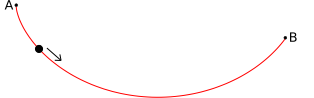
\includegraphics[scale=0.5]{images/Brachistochrone.png}
	\caption{Curva Braquistócrona}
	\label{fig:brachistochrone}
\end{figure}

\indent Este problema apenas é válido quando se consideram pares de pontos com a altura de B inferior à de A, pois caso contrário o corpo não consegue efectuar o percurso.

Leibniz, L'Hospital, Newton, e os irmãos Bernoulli apresentaram soluções analíticas.
No entanto o estudo deste problema, segundo o paradigma de agentes adaptativos, é interessante pois permite calcular uma aproximação da curva
não necessitando de ferramentas matemáticas complexas.

\indent Para cada instância do problema, um indivíduo representa uma trajectória possível. Estes individuos são avaliados segundo uma
função de aptidão que mede o tempo correspondente: quanto menor, mais apto ele é considerado.

\indent De forma a definir o o formato da trajectória, cada indivíduo é caracterizado por um conjunto de genes. Estes representam os vários
factores que contribuem para a forma da trajectória, como por exemplo coordenadas, declives, curvaturas, etc. Assim, para alterar as características
de um determinado indivíduo (fenótipo) é necessário efectuar alterações ao seu conjunto genético (genótipo). Estas alterações podem se categorizar
fundamentalmente em dois tipos:

\begin{description}
	\item[Mutation] \hfill \\ 
		Alteração ou substituição de um gene por outro de origem primariamente estocástica.
	\item[Crossover] \hfill \\ 
		Aplicação de permutações no código genético de dois ou mais indivíduos, trocando a informação genética de um para outro.
\end{description}

\cleardoublepage
\section{Implementation}
\indent \indent Durante a implementação deste projecto foram surgindo abordagens alternativas,
introduzidas tanto por erros conceptuais, como por \emph{bugs}. Estas abordagens, apesar de não estarem de acordo com
o considerado comum na àrea de Inteligência Artificial, foram demonstrando capacidade de gerar soluções adequadas ao problema.
Assim, decidimos que seria interessante efectuar uma comparação entre os resultados obtidos segundo o método tradicional, e aquele a que apelidámos \emph{Rafael-Ribeiro}. 

\subsection{Representation}
\indent \indent À semelhança de outros problemas\footnote[1]{Aplicação do método do trapézio para o cálculo do integral de uma curva.}, a discretização do espaço contínuo em amostras
distintas facilita a computação numérica dos resultados. Desta forma escolhemos implementar duas formas de representação:

\begin{description}
	\item[Fixed] \hfill \\ 
		Onde a curva é aproximada por um conjunto sucessivo de segmentos de recta, definidos por pares de pontos equidistantes.
	\item[Dynamic] \hfill \\ 
		Uma representação da mesma natureza que a anterior, apenas retirando a restrição da distância entre pontos.
\end{description}

\indent Estas duas representações foram escolhidas por serem compactas, i.e.: para cada gene apenas é necessário guardar a informação das suas coordenadas.
Note-se que no caso da representação fixa a absissa é conhecida \emph{a priori}, reduzindo assim o espaço de procura exponencialmente (em relação à dinâmica).

\indent Para além destas duas representações considerámos ainda uma terceira:

\begin{description}
	\item[NURBS] \hfill \\ 
		A curva aproximada é definida à custa dos pontos de controlo de uma NURBS\footnote[2]{Non-uniform rational basis spline.}. 
		\begin{figure}[ht]
			\centering
			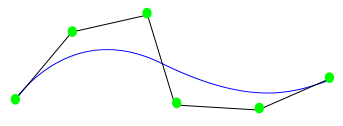
\includegraphics[scale=0.50]{images/NURBstatic.png}
			\caption{Exemplo de uma NURBS}
			\label{fig:nurbs}
		\end{figure}
\end{description}

\indent A principal vantagem desta representação é o facto de se basear em polinómios de grau superior a um, o que permite aproximar a curva desejada
com igual rigor utilizando um conjunto de pontos inferior. Desta forma o espaço de procura é mais reduzido, pelo que a convergência do algoritmo
seria esperadamente mais rápida.

\indent No entanto esta representação também apresenta os seus problemas: a avaliação da aptidão de um indivíduo depende do cálculo da derivada
desta curva, o que representa por si só um problema merecedor de uma análise profunda. 

\cleardoublepage
\subsection{Mutation Operators}
\indent \indent Um dos principais factores que contribuem para a performance de um algoritmo genético é a diversidade genética presente na população.
Desta forma, desenvolver os operadores de mutação adequados para cada problema torna-se uma tarefa crucial.
Estes actuam ao nível de cada gene e são portanto distintos para cada representação. 

\subsubsection{Fixed Representation}
\indent \indent Nesta representação o único parâmetro que se altera são as coordenadas \emph{yy} de cada gene.
Para sortear o novo valor a atribuir foi utilizada uma distribuição gaussiana (ao invés de uniforme), com o intuito 
de garantir que a evolução progenitor-filho é efectuada de forma gradual (i.e.: que o filho preserva algumas características dos
seus antecessores).

\subsubsection{Dynamic Representation}
\indent \indent Ao contrário da representação anterior, o operador de mutação para a representação dinâmica necessíta de considerar
tanto as coordenadas \emph{yy} como as \emph{xx}. Pelas razões já enunciadas, a distribuição utilizada foi novamente a gaussiana.
No entanto, uma vez que esta permite alterar a posição relativa dos pontos, é necessário efectuar um ordenamento posterior.

\indent Como estes operadores se aplicam a genes individualmente, é necessário escolher quais genes sofrem mutação.
O operador tradicional aplica uma igual probabilidade a cada gene. No entanto, segundo o paradigma biológico,
a probabilidade de erros consecutivos é mais elevada (pois a anomalia que levou à criação do primeiro erro pode ainda verificar-se).
Como achamos que esta abordagem poderia ser vantajosa para o problema em questão, decidimos implementar dois modelos de mutações adicionais:

\begin{description}
	\item[Burst] \hfill \\ 
		Onde indicamos a probabilidade de um gene ser mutado após o seu antecessor também o ser.

	\item[Range] \hfill \\ 
		Onde por cada indivíduo é apenas selecionado uma secção de genes que sofre mutação.
		Este tipo de mutação é apenas aplicado para o tipo de selecção \emph{Rafael-Ribeiro}.
\end{description}
 
\cleardoublepage
\subsection{Crossover Operator}
\indent \indent O operador de recombinação distingue-se do operador de mutação na forma como tem impacto no material genético da população.
Enquanto que o operador de mutação actua sobre um único indivíduo (o que introduz novo material genético na população),
o operador de recombinação reorganiza o material genético já existente, conseguindo propagar as características entre indivíduos.
Este operador aliado a um tipo de selecção adequado (ver \ref{subsec:selection}) permite uma melhor convergência
do algoritmo.

\subsubsection{Fixed Representation}
\indent \indent 

\subsubsection{Dynamic Representation}
\indent \indent 

\cleardoublepage
\subsection{Selection}
\label{subsec:selection}
\indent \indent Após a criação de novos descendentes é necessário efectuar uma redução no número de indivíduos.
Desta forma é possível garantir que o tamanho da população continua computacionalmente tratável e que o algoritmo convirja tendencialmente para o óptimo global.

\begin{description}
	\item[Elitism] \hfill \\
		Abordagem gananciosa que seleciona os melhores indivíduos da população como descendetes.

	\item[Roulette] \hfill \\
		Os indivíduos são selecionados de forma aleatória, dando maior probabilidade aos indivíduos com maior fitness.
		Para garantir esta propriedade a função de probabilidade para um indivíduo $i$ é:

		\[
			p_{i} = \frac{f_{i}}{\sum\limits_{j \in \text{Pop.}} f_{j}} \quad \text{onde} \quad f_i = \frac{1}{T_{i}} \quad (T_{i} \leftarrow \text{Tempo correspondente ao indivíduo } i)
		\]

		Neste algoritmo o mesmo elemento pode ser escolhido várias vezes,
		simulando a capacidade de um ser mais apto se conseguir reproduzir com maior frequência.

	\item[Tournament] \hfill \\ 
		Para este tipo de selecção são escolhidos aleatoriamente N indivíduos, dos quais apenas o mais apto é escolhido.
		Após esta selecção todos os elementos participantes no torneiao são devolvidos à população.

	\item[Rafael-Ribeiro] \hfill \\ 
		Nesta abordagem implementa-se em conjunto a selecção por elitismo e por torneio, mas ao contrário da abordagem tradicional
		esta é aplicada não só para selecionar os progenitores, mas também para selecionar que indivíduos da população inteira (pais e filhos)
		sobrevivem para a próxima iteração. Do ponto de vista em que apenas alguns indivíduos são alterados este tipo de selecção pode ser considerada \emph{Steady-State}.

\end{description}

\indent \indent 


\cleardoublepage

\subsection{...}
\indent \indent ...

\subsection{...}
\indent \indent ...

\subsubsection{...}
\indent \indent ...

\subsubsection{...}
\indent \indent ...

...

\cleardoublepage
\subsection{...}
\indent \indent ...

...

\subsection{...}
\indent \indent ...

...

\subsection{...}
\indent \indent ...

\cleardoublepage

\section{Experiments}
\indent \indent ...

\cleardoublepage

\subsection{...}
\indent \indent ...

\cleardoublepage

\section{Validation}
\indent \indent Para validar o comportamento do Agente, cada combinação de parâmetros foi executada 30 vezes com seeds diferentes;
tal garante que a natureza estocástica do algoritmo fica evidenciada ao garantir que os testes são, de facto, diferentes.

Após a conclusão dos testes, foi calculado o desvio-padrão entre as 30 simulações,
para averiguar se os resultados obtidos não representavam apenas um caso de sorte.

Tal como se pode verificar na última coluna da tabela de resultados (Secção \ref{tab:results}), o desvio-padrão entre as 30 simulações para cada combinação de parâmetros
é bastante reduzido, o que comprova a sua consistência e robustez.

\cleardoublepage

\subsection{...}
\indent \indent ...

\cleardoublepage

\section{Result Analysis}
\indent \indent ...

\cleardoublepage

\subsection{...}
\indent \indent ...

\cleardoublepage
\section{Conclusion}
\indent \indent ...

\cleardoublepage

\subsection{...}
\indent \indent ...

\cleardoublepage
\section{Anexos}

\eject \pdfpagewidth=594.0mm \pdfpageheight=420.0mm

\subsection{Tabela de Resultados}
\begin{center}
	\begin{longtable}{ | c | c | c | c | c | c | c | c | c | c | c | c | c | c | c | c | c | }
	\hline
	\textbf{Points set}	&	\textbf{Representation}	&	\textbf{Selection Type}	&	\textbf{No. pts.}	&	\textbf{Pop. size}	&	\textbf{Elitism  (\%)}	&	\textbf{Crossover Prob. (\%)}	&	\textbf{No. pts. Crossover}	&	\textbf{Prob. Mutation (\%)}	&	\textbf{Best (20)}	&	\textbf{Best (100)}	&	\textbf{Best (1000)}	&	\textbf{Best (2000)}	&	\textbf{Average (2000)}	&	\textbf{Worst (2000)}	&	\textbf{Std. Dev. (2000, Pop.)}	&	\textbf{Std. Dev. x100 (2000, 30 runs)} \\
	\hline
	\hline
	1	&	Dynamic	&	Tournament	&	15	&	25	&	5.00	&	0.00	&	NA	&	5.00	&	1.7798555	&	1.3804207	&	1.2214826	&	1.2171368	&	1.2855872	&	1.8891135	&	0.1423133	&	0.1569723 \\
	\hline
	1	&	Dynamic	&	Tournament	&	15	&	25	&	5.00	&	0.00	&	NA	&	25.00	&	1.6387113	&	1.3374381	&	1.2294197	&	1.2240526	&	1.5092776	&	1.9289822	&	0.1856915	&	0.5851234 \\
	\hline
	1	&	Dynamic	&	Tournament	&	15	&	25	&	5.00	&	35.00	&	2	&	5.00	&	1.7645611	&	1.3846251	&	1.2235878	&	1.2178209	&	1.2755522	&	1.5378397	&	0.0731764	&	0.2559497 \\
	\hline
	1	&	Dynamic	&	Tournament	&	15	&	25	&	5.00	&	35.00	&	2	&	25.00	&	1.6366198	&	1.3489135	&	1.2306325	&	1.2241706	&	1.5815125	&	3.2559805	&	0.4413373	&	0.7620405 \\
	\hline
	1	&	Dynamic	&	Tournament	&	15	&	25	&	5.00	&	35.00	&	5	&	5.00	&	1.7549878	&	1.3941534	&	1.2222179	&	1.2179503	&	1.2753718	&	1.5528651	&	0.0755826	&	0.2365574 \\
	\hline
	1	&	Dynamic	&	Tournament	&	15	&	25	&	5.00	&	35.00	&	5	&	25.00	&	1.5997140	&	1.3169590	&	1.2312039	&	1.2253416	&	1.5561979	&	2.8622221	&	0.3605938	&	0.6181510 \\
	\hline
	1	&	Dynamic	&	Tournament	&	15	&	25	&	20.00	&	0.00	&	NA	&	5.00	&	1.7071056	&	1.3596559	&	1.2178007	&	1.2153561	&	1.2384174	&	1.4464642	&	0.0544712	&	0.1049954 \\
	\hline
	1	&	Dynamic	&	Tournament	&	15	&	25	&	20.00	&	0.00	&	NA	&	25.00	&	1.5775374	&	1.2914149	&	1.2230546	&	1.2194394	&	1.3333207	&	1.6977337	&	0.1257296	&	0.2242895 \\
	\hline
	1	&	Dynamic	&	Tournament	&	15	&	25	&	20.00	&	35.00	&	2	&	5.00	&	1.7568935	&	1.3711726	&	1.2181654	&	1.2152563	&	1.2435227	&	1.5839707	&	0.0801040	&	0.0964408 \\
	\hline
	1	&	Dynamic	&	Tournament	&	15	&	25	&	20.00	&	35.00	&	2	&	25.00	&	1.5664255	&	1.2805528	&	1.2250549	&	1.2206995	&	1.3494917	&	1.7543654	&	0.1435915	&	0.4044988 \\
	\hline
	1	&	Dynamic	&	Tournament	&	15	&	25	&	20.00	&	35.00	&	5	&	5.00	&	1.7142195	&	1.3411961	&	1.2175074	&	1.2151081	&	1.2483471	&	1.5921128	&	0.0860409	&	0.0938125 \\
	\hline
	1	&	Dynamic	&	Tournament	&	15	&	25	&	20.00	&	35.00	&	5	&	25.00	&	1.5924041	&	1.2946479	&	1.2234791	&	1.2193236	&	1.3530618	&	1.8036510	&	0.1517908	&	0.3063623 \\
	\hline
	1	&	Dynamic	&	Tournament	&	15	&	50	&	5.00	&	0.00	&	NA	&	5.00	&	1.6779650	&	1.3591788	&	1.2239797	&	1.2182432	&	1.3901535	&	1.8152864	&	0.1432619	&	0.3508536 \\
	\hline
	1	&	Dynamic	&	Tournament	&	15	&	50	&	5.00	&	0.00	&	NA	&	25.00	&	1.5739769	&	1.3269143	&	1.2310873	&	1.2234359	&	1.7627173	&	2.4092700	&	0.2931448	&	0.4940614 \\
	\hline
	1	&	Dynamic	&	Tournament	&	15	&	50	&	5.00	&	35.00	&	2	&	5.00	&	1.6574976	&	1.3652564	&	1.2220822	&	1.2180924	&	1.4018081	&	2.2147800	&	0.1984693	&	0.3499979 \\
	\hline
	1	&	Dynamic	&	Tournament	&	15	&	50	&	5.00	&	35.00	&	2	&	25.00	&	1.5733395	&	1.3194227	&	1.2316545	&	1.2245416	&	1.8001901	&	4.0780631	&	0.5095846	&	0.8556297 \\
	\hline
	1	&	Dynamic	&	Tournament	&	15	&	50	&	5.00	&	35.00	&	5	&	5.00	&	1.6570812	&	1.3408675	&	1.2210690	&	1.2172407	&	1.4015002	&	2.1589754	&	0.1863246	&	0.2608487 \\
	\hline
	1	&	Dynamic	&	Tournament	&	15	&	50	&	5.00	&	35.00	&	5	&	25.00	&	1.5473851	&	1.3247167	&	1.2318544	&	1.2243604	&	1.7338216	&	2.7922778	&	0.3339150	&	0.6634347 \\
	\hline
	1	&	Dynamic	&	Tournament	&	15	&	50	&	20.00	&	0.00	&	NA	&	5.00	&	1.6078798	&	1.2990023	&	1.2161943	&	1.2144174	&	1.2460124	&	1.6751434	&	0.0830522	&	0.0608947 \\
	\hline
	1	&	Dynamic	&	Tournament	&	15	&	50	&	20.00	&	0.00	&	NA	&	25.00	&	1.4786964	&	1.2645791	&	1.2217304	&	1.2184489	&	1.4166767	&	2.7871974	&	0.2909448	&	0.3414112 \\
	\hline
	1	&	Dynamic	&	Tournament	&	15	&	50	&	20.00	&	35.00	&	2	&	5.00	&	1.5905558	&	1.3096392	&	1.2162614	&	1.2144527	&	1.2530232	&	1.9220403	&	0.1190049	&	0.0574027 \\
	\hline
	1	&	Dynamic	&	Tournament	&	15	&	50	&	20.00	&	35.00	&	2	&	25.00	&	1.4909638	&	1.2580901	&	1.2204253	&	1.2180191	&	1.3972693	&	2.6893642	&	0.2659871	&	0.2524264 \\
	\hline
	1	&	Dynamic	&	Tournament	&	15	&	50	&	20.00	&	35.00	&	5	&	5.00	&	1.5983842	&	1.3041431	&	1.2168150	&	1.2147173	&	1.2497317	&	1.7564688	&	0.0948583	&	0.0787589 \\
	\hline
	1	&	Dynamic	&	Tournament	&	15	&	50	&	20.00	&	35.00	&	5	&	25.00	&	1.5005366	&	1.2666354	&	1.2207167	&	1.2176385	&	1.4062357	&	2.7415784	&	0.2743122	&	0.2207026 \\
	\hline
	1	&	Dynamic	&	Tournament	&	15	&	100	&	5.00	&	0.00	&	NA	&	5.00	&	1.5584232	&	1.2977242	&	1.2177620	&	1.2151850	&	1.3377928	&	2.3506955	&	0.1625919	&	0.0993585 \\
	\hline
	1	&	Dynamic	&	Tournament	&	15	&	100	&	5.00	&	0.00	&	NA	&	25.00	&	1.4597030	&	1.2617386	&	1.2223083	&	1.2189487	&	1.6976760	&	3.9941744	&	0.4365012	&	0.2988285 \\
	\hline
	1	&	Dynamic	&	Tournament	&	15	&	100	&	5.00	&	35.00	&	2	&	5.00	&	1.5430401	&	1.2867505	&	1.2176236	&	1.2152363	&	1.3303994	&	1.9426754	&	0.1261230	&	0.1099206 \\
	\hline
	1	&	Dynamic	&	Tournament	&	15	&	100	&	5.00	&	35.00	&	2	&	25.00	&	1.4803913	&	1.2657400	&	1.2234430	&	1.2193863	&	1.6750848	&	4.7410434	&	0.4686266	&	0.3027827 \\
	\hline
	1	&	Dynamic	&	Tournament	&	15	&	100	&	5.00	&	35.00	&	5	&	5.00	&	1.5515495	&	1.2900368	&	1.2184431	&	1.2153366	&	1.3438610	&	1.9015783	&	0.1250422	&	0.0949568 \\
	\hline
	1	&	Dynamic	&	Tournament	&	15	&	100	&	5.00	&	35.00	&	5	&	25.00	&	1.4731484	&	1.2656088	&	1.2224566	&	1.2196624	&	1.6389763	&	3.0345345	&	0.3051621	&	0.3502439 \\
	\hline
	1	&	Dynamic	&	Tournament	&	15	&	100	&	20.00	&	0.00	&	NA	&	5.00	&	1.5089657	&	1.2591590	&	1.2152843	&	1.2141346	&	1.2499208	&	1.7710180	&	0.0934463	&	0.0664633 \\
	\hline
	1	&	Dynamic	&	Tournament	&	15	&	100	&	20.00	&	0.00	&	NA	&	25.00	&	1.4306861	&	1.2447508	&	1.2181126	&	1.2162282	&	1.4217654	&	4.1642367	&	0.3837596	&	0.1675580 \\
	\hline
	1	&	Dynamic	&	Tournament	&	15	&	100	&	20.00	&	35.00	&	2	&	5.00	&	1.5204479	&	1.2623009	&	1.2153587	&	1.2140487	&	1.2472616	&	1.8195834	&	0.0910645	&	0.0653385 \\
	\hline
	1	&	Dynamic	&	Tournament	&	15	&	100	&	20.00	&	35.00	&	2	&	25.00	&	1.4389591	&	1.2487813	&	1.2186170	&	1.2166224	&	1.4005038	&	3.1380292	&	0.2733357	&	0.1470783 \\
	\hline
	1	&	Dynamic	&	Tournament	&	15	&	100	&	20.00	&	35.00	&	5	&	5.00	&	1.5048529	&	1.2673824	&	1.2153698	&	1.2140683	&	1.2517682	&	2.1992441	&	0.1275911	&	0.0402102 \\
	\hline
	1	&	Dynamic	&	Tournament	&	15	&	100	&	20.00	&	35.00	&	5	&	25.00	&	1.4394328	&	1.2482233	&	1.2193379	&	1.2170282	&	1.3887502	&	2.3375056	&	0.1933840	&	0.1852128 \\
	\hline
	1	&	Dynamic	&	Tournament	&	30	&	25	&	5.00	&	0.00	&	NA	&	5.00	&	3.0241153	&	2.2870420	&	1.5261449	&	1.3493051	&	1.5935519	&	2.0557476	&	0.1858032	&	7.8105710 \\
	\hline
	1	&	Dynamic	&	Tournament	&	30	&	25	&	5.00	&	0.00	&	NA	&	25.00	&	2.9892652	&	2.3966830	&	1.8011931	&	1.6516420	&	2.8222093	&	3.9452314	&	0.5841092	&	18.5965986 \\
	\hline
	1	&	Dynamic	&	Tournament	&	30	&	25	&	5.00	&	35.00	&	2	&	5.00	&	2.9944279	&	2.2714349	&	1.5017791	&	1.3624134	&	1.6238496	&	2.1611009	&	0.2061994	&	10.1997876 \\
	\hline
	1	&	Dynamic	&	Tournament	&	30	&	25	&	5.00	&	35.00	&	2	&	25.00	&	2.9637315	&	2.4028335	&	1.7987249	&	1.6562247	&	2.8073140	&	4.2412314	&	0.6476271	&	20.1348564 \\
	\hline
	1	&	Dynamic	&	Tournament	&	30	&	25	&	5.00	&	35.00	&	5	&	5.00	&	3.0334155	&	2.3078157	&	1.5169478	&	1.3662690	&	1.6250130	&	2.0575869	&	0.1896045	&	8.5788800 \\
	\hline
	1	&	Dynamic	&	Tournament	&	30	&	25	&	5.00	&	35.00	&	5	&	25.00	&	3.0521300	&	2.3782740	&	1.7726390	&	1.6618767	&	2.7643008	&	3.8716787	&	0.5660606	&	21.7655209 \\
	\hline
	1	&	Dynamic	&	Tournament	&	30	&	25	&	20.00	&	0.00	&	NA	&	5.00	&	2.9539978	&	2.1024998	&	1.3519152	&	1.2628652	&	1.3420289	&	1.8731640	&	0.1413552	&	3.6082740 \\
	\hline
	1	&	Dynamic	&	Tournament	&	30	&	25	&	20.00	&	0.00	&	NA	&	25.00	&	2.8256159	&	2.1885145	&	1.6509152	&	1.5287695	&	2.0324691	&	3.3636243	&	0.4852465	&	17.7621368 \\
	\hline
	1	&	Dynamic	&	Tournament	&	30	&	25	&	20.00	&	35.00	&	2	&	5.00	&	2.9140885	&	2.1317807	&	1.3912177	&	1.2900100	&	1.3650007	&	1.7495199	&	0.1145554	&	5.7359827 \\
	\hline
	1	&	Dynamic	&	Tournament	&	30	&	25	&	20.00	&	35.00	&	2	&	25.00	&	2.8855914	&	2.1740878	&	1.5921175	&	1.4947861	&	1.9830452	&	3.4054299	&	0.4880600	&	14.9423265 \\
	\hline
	1	&	Dynamic	&	Tournament	&	30	&	25	&	20.00	&	35.00	&	5	&	5.00	&	2.9489919	&	2.1012636	&	1.3534723	&	1.2743137	&	1.3479058	&	1.7043310	&	0.1063730	&	4.6961729 \\
	\hline
	1	&	Dynamic	&	Tournament	&	30	&	25	&	20.00	&	35.00	&	5	&	25.00	&	2.8911136	&	2.1482890	&	1.5624525	&	1.4742001	&	1.9301330	&	2.6171929	&	0.3439067	&	14.1575000 \\
	\hline
	1	&	Dynamic	&	Tournament	&	30	&	50	&	5.00	&	0.00	&	NA	&	5.00	&	2.9820616	&	2.1976345	&	1.4638068	&	1.3451448	&	1.9028023	&	3.1948918	&	0.4139098	&	8.7382751 \\
	\hline
	1	&	Dynamic	&	Tournament	&	30	&	50	&	5.00	&	0.00	&	NA	&	25.00	&	3.0034802	&	2.3564119	&	1.7758596	&	1.6488573	&	3.2832022	&	4.4628544	&	0.6538322	&	18.0427582 \\
	\hline
	1	&	Dynamic	&	Tournament	&	30	&	50	&	5.00	&	35.00	&	2	&	5.00	&	2.9723681	&	2.2320806	&	1.4687581	&	1.3444392	&	1.9168218	&	2.7218863	&	0.3499373	&	7.4816034 \\
	\hline
	1	&	Dynamic	&	Tournament	&	30	&	50	&	5.00	&	35.00	&	2	&	25.00	&	2.9259580	&	2.3955879	&	1.8552572	&	1.7427870	&	3.5077731	&	6.1051042	&	0.8377945	&	22.4558609 \\
	\hline
	1	&	Dynamic	&	Tournament	&	30	&	50	&	5.00	&	35.00	&	5	&	5.00	&	3.0008071	&	2.2872974	&	1.5014871	&	1.3553037	&	1.9173880	&	2.7280623	&	0.3427520	&	9.9224450 \\
	\hline
	1	&	Dynamic	&	Tournament	&	30	&	50	&	5.00	&	35.00	&	5	&	25.00	&	2.9592536	&	2.3321408	&	1.7415598	&	1.6248364	&	3.2725527	&	4.6691223	&	0.6864720	&	16.4034541 \\
	\hline
	1	&	Dynamic	&	Tournament	&	30	&	50	&	20.00	&	0.00	&	NA	&	5.00	&	2.7942350	&	1.9568596	&	1.3315192	&	1.2539519	&	1.3404724	&	1.9544724	&	0.1320934	&	2.4978841 \\
	\hline
	1	&	Dynamic	&	Tournament	&	30	&	50	&	20.00	&	0.00	&	NA	&	25.00	&	2.7053609	&	1.9250811	&	1.4502105	&	1.3762398	&	1.9260496	&	4.0336877	&	0.5569000	&	8.8982337 \\
	\hline
	1	&	Dynamic	&	Tournament	&	30	&	50	&	20.00	&	35.00	&	2	&	5.00	&	2.7947838	&	1.9768370	&	1.3333488	&	1.2610420	&	1.3453404	&	1.7543229	&	0.1055524	&	3.8732595 \\
	\hline
	1	&	Dynamic	&	Tournament	&	30	&	50	&	20.00	&	35.00	&	2	&	25.00	&	2.7260588	&	1.9821525	&	1.4704425	&	1.3956011	&	1.8817648	&	2.6872210	&	0.3542646	&	10.2229845 \\
	\hline
	1	&	Dynamic	&	Tournament	&	30	&	50	&	20.00	&	35.00	&	5	&	5.00	&	2.8228348	&	1.9838148	&	1.3309642	&	1.2555107	&	1.3407083	&	1.8394806	&	0.1141787	&	3.1595486 \\
	\hline
	1	&	Dynamic	&	Tournament	&	30	&	50	&	20.00	&	35.00	&	5	&	25.00	&	2.7117558	&	1.9953746	&	1.5032434	&	1.4207996	&	1.9737368	&	3.5947762	&	0.4675957	&	13.6142756 \\
	\hline
	1	&	Dynamic	&	Tournament	&	30	&	100	&	5.00	&	0.00	&	NA	&	5.00	&	2.7603940	&	1.9784741	&	1.3422039	&	1.2772740	&	1.6166756	&	2.5409931	&	0.2532344	&	4.8995051 \\
	\hline
	1	&	Dynamic	&	Tournament	&	30	&	100	&	5.00	&	0.00	&	NA	&	25.00	&	2.7162829	&	2.0087901	&	1.5505925	&	1.4656556	&	2.6675271	&	4.3925622	&	0.5927422	&	15.8928720 \\
	\hline
	1	&	Dynamic	&	Tournament	&	30	&	100	&	5.00	&	35.00	&	2	&	5.00	&	2.7399697	&	2.0250188	&	1.3517838	&	1.2687510	&	1.5949186	&	2.4785520	&	0.2454454	&	4.7645855 \\
	\hline
	1	&	Dynamic	&	Tournament	&	30	&	100	&	5.00	&	35.00	&	2	&	25.00	&	2.6135124	&	1.9763409	&	1.5522914	&	1.4706218	&	2.7402147	&	4.8428890	&	0.6463274	&	15.8192247 \\
	\hline
	1	&	Dynamic	&	Tournament	&	30	&	100	&	5.00	&	35.00	&	5	&	5.00	&	2.7861186	&	1.9806727	&	1.3340448	&	1.2654976	&	1.6121063	&	2.4439884	&	0.2486804	&	4.4538031 \\
	\hline
	1	&	Dynamic	&	Tournament	&	30	&	100	&	5.00	&	35.00	&	5	&	25.00	&	2.7095274	&	2.0570141	&	1.4825159	&	1.4073239	&	2.5495027	&	3.7207713	&	0.5420656	&	11.4028266 \\
	\hline
	1	&	Dynamic	&	Tournament	&	30	&	100	&	20.00	&	0.00	&	NA	&	5.00	&	2.6078851	&	1.8262564	&	1.2911006	&	1.2391886	&	1.3222918	&	1.9202444	&	0.1177234	&	1.8183417 \\
	\hline
	1	&	Dynamic	&	Tournament	&	30	&	100	&	20.00	&	0.00	&	NA	&	25.00	&	2.5086127	&	1.7929367	&	1.3918626	&	1.3352990	&	1.8102752	&	3.2678144	&	0.3980121	&	8.6783465 \\
	\hline
	1	&	Dynamic	&	Tournament	&	30	&	100	&	20.00	&	35.00	&	2	&	5.00	&	2.6296208	&	1.8270909	&	1.2817181	&	1.2333926	&	1.3138706	&	1.8325179	&	0.1093286	&	1.9645085 \\
	\hline
	1	&	Dynamic	&	Tournament	&	30	&	100	&	20.00	&	35.00	&	2	&	25.00	&	2.5614479	&	1.8230046	&	1.4073011	&	1.3538573	&	1.8214754	&	4.0144986	&	0.4419204	&	9.0195337 \\
	\hline
	1	&	Dynamic	&	Tournament	&	30	&	100	&	20.00	&	35.00	&	5	&	5.00	&	2.6274094	&	1.8301547	&	1.2899317	&	1.2388849	&	1.3222765	&	2.0995080	&	0.1304264	&	1.8085610 \\
	\hline
	1	&	Dynamic	&	Tournament	&	30	&	100	&	20.00	&	35.00	&	5	&	25.00	&	2.5075852	&	1.7811631	&	1.3936121	&	1.3454511	&	1.8009246	&	3.1117900	&	0.3667037	&	8.3174459 \\
	\hline
	1	&	Dynamic	&	Roulette	&	15	&	25	&	5.00	&	0.00	&	NA	&	5.00	&	1.7428558	&	1.3907379	&	1.2221460	&	1.2176776	&	1.2831480	&	1.6135393	&	0.0896902	&	0.2221814 \\
	\hline
	1	&	Dynamic	&	Roulette	&	15	&	25	&	5.00	&	0.00	&	NA	&	25.00	&	1.6270911	&	1.3158784	&	1.2312508	&	1.2233814	&	1.5787696	&	3.1214934	&	0.4123084	&	0.5164064 \\
	\hline
	1	&	Dynamic	&	Roulette	&	15	&	25	&	5.00	&	35.00	&	2	&	5.00	&	1.7616388	&	1.4037228	&	1.2223646	&	1.2174774	&	1.2730297	&	1.5881841	&	0.0832034	&	0.1910814 \\
	\hline
	1	&	Dynamic	&	Roulette	&	15	&	25	&	5.00	&	35.00	&	2	&	25.00	&	1.6398489	&	1.3389605	&	1.2290112	&	1.2235723	&	1.5438479	&	2.7500535	&	0.3435471	&	0.5140365 \\
	\hline
	1	&	Dynamic	&	Roulette	&	15	&	25	&	5.00	&	35.00	&	5	&	5.00	&	1.7216297	&	1.3608354	&	1.2208705	&	1.2172250	&	1.3037182	&	2.2094351	&	0.2048888	&	0.2008811 \\
	\hline
	1	&	Dynamic	&	Roulette	&	15	&	25	&	5.00	&	35.00	&	5	&	25.00	&	1.5875229	&	1.3263148	&	1.2308108	&	1.2243531	&	1.5789210	&	2.6740883	&	0.3308117	&	0.5167461 \\
	\hline
	1	&	Dynamic	&	Roulette	&	15	&	25	&	20.00	&	0.00	&	NA	&	5.00	&	1.7484987	&	1.3541369	&	1.2178021	&	1.2151325	&	1.2505549	&	1.7122481	&	0.1055554	&	0.0790360 \\
	\hline
	1	&	Dynamic	&	Roulette	&	15	&	25	&	20.00	&	0.00	&	NA	&	25.00	&	1.5812460	&	1.2853418	&	1.2239918	&	1.2203170	&	1.3649368	&	2.2403135	&	0.2316100	&	0.4082052 \\
	\hline
	1	&	Dynamic	&	Roulette	&	15	&	25	&	20.00	&	35.00	&	2	&	5.00	&	1.7461313	&	1.3813756	&	1.2180799	&	1.2152846	&	1.2393712	&	1.4777937	&	0.0602246	&	0.0709448 \\
	\hline
	1	&	Dynamic	&	Roulette	&	15	&	25	&	20.00	&	35.00	&	2	&	25.00	&	1.5956923	&	1.2951400	&	1.2244794	&	1.2201828	&	1.3511049	&	1.8064734	&	0.1522716	&	0.4562409 \\
	\hline
	1	&	Dynamic	&	Roulette	&	15	&	25	&	20.00	&	35.00	&	5	&	5.00	&	1.7280689	&	1.3699736	&	1.2184602	&	1.2153689	&	1.2391900	&	1.4836848	&	0.0613522	&	0.1093037 \\
	\hline
	1	&	Dynamic	&	Roulette	&	15	&	25	&	20.00	&	35.00	&	5	&	25.00	&	1.5821089	&	1.3081968	&	1.2232304	&	1.2192104	&	1.3500189	&	1.7992047	&	0.1496290	&	0.2755991 \\
	\hline
	1	&	Dynamic	&	Roulette	&	15	&	50	&	5.00	&	0.00	&	NA	&	5.00	&	1.6627745	&	1.3503424	&	1.2222896	&	1.2178707	&	1.3903998	&	1.7328154	&	0.1301884	&	0.2224996 \\
	\hline
	1	&	Dynamic	&	Roulette	&	15	&	50	&	5.00	&	0.00	&	NA	&	25.00	&	1.5484784	&	1.3105168	&	1.2295210	&	1.2238031	&	1.8289541	&	4.6330684	&	0.5947717	&	0.5005507 \\
	\hline
	1	&	Dynamic	&	Roulette	&	15	&	50	&	5.00	&	35.00	&	2	&	5.00	&	1.6581429	&	1.3723184	&	1.2220793	&	1.2176520	&	1.3985260	&	1.8241810	&	0.1434455	&	0.1940176 \\
	\hline
	1	&	Dynamic	&	Roulette	&	15	&	50	&	5.00	&	35.00	&	2	&	25.00	&	1.5532844	&	1.3116116	&	1.2301845	&	1.2244249	&	1.7833691	&	3.0999511	&	0.3738119	&	0.5251096 \\
	\hline
	1	&	Dynamic	&	Roulette	&	15	&	50	&	5.00	&	35.00	&	5	&	5.00	&	1.6762995	&	1.3566805	&	1.2205564	&	1.2170021	&	1.3974064	&	1.8765936	&	0.1515107	&	0.2569220 \\
	\hline
	1	&	Dynamic	&	Roulette	&	15	&	50	&	5.00	&	35.00	&	5	&	25.00	&	1.5775049	&	1.3271575	&	1.2321838	&	1.2245138	&	1.7865066	&	3.6395958	&	0.4422532	&	0.5792444 \\
	\hline
	1	&	Dynamic	&	Roulette	&	15	&	50	&	20.00	&	0.00	&	NA	&	5.00	&	1.5762381	&	1.2945880	&	1.2166823	&	1.2147015	&	1.2507886	&	1.8021717	&	0.1037473	&	0.0723439 \\
	\hline
	1	&	Dynamic	&	Roulette	&	15	&	50	&	20.00	&	0.00	&	NA	&	25.00	&	1.4779650	&	1.2647266	&	1.2215084	&	1.2184853	&	1.3941109	&	2.6456148	&	0.2533046	&	0.2440008 \\
	\hline
	1	&	Dynamic	&	Roulette	&	15	&	50	&	20.00	&	35.00	&	2	&	5.00	&	1.5808428	&	1.2940802	&	1.2166121	&	1.2147142	&	1.2480274	&	1.7203776	&	0.0891606	&	0.0833979 \\
	\hline
	1	&	Dynamic	&	Roulette	&	15	&	50	&	20.00	&	35.00	&	2	&	25.00	&	1.4796395	&	1.2599873	&	1.2209803	&	1.2182362	&	1.3912172	&	2.1360482	&	0.1890859	&	0.3058145 \\
	\hline
	1	&	Dynamic	&	Roulette	&	15	&	50	&	20.00	&	35.00	&	5	&	5.00	&	1.5805124	&	1.3077502	&	1.2164494	&	1.2146498	&	1.2492966	&	1.7803488	&	0.0980238	&	0.0822618 \\
	\hline
	1	&	Dynamic	&	Roulette	&	15	&	50	&	20.00	&	35.00	&	5	&	25.00	&	1.4786673	&	1.2705444	&	1.2211162	&	1.2179348	&	1.4038069	&	2.6132760	&	0.2627397	&	0.2477049 \\
	\hline
	1	&	Dynamic	&	Roulette	&	15	&	100	&	5.00	&	0.00	&	NA	&	5.00	&	1.5459077	&	1.2923318	&	1.2168381	&	1.2150528	&	1.3260713	&	1.8223520	&	0.1094464	&	0.0971595 \\
	\hline
	1	&	Dynamic	&	Roulette	&	15	&	100	&	5.00	&	0.00	&	NA	&	25.00	&	1.4614524	&	1.2742082	&	1.2231204	&	1.2199268	&	1.6548993	&	3.2009502	&	0.3220925	&	0.4504934 \\
	\hline
	1	&	Dynamic	&	Roulette	&	15	&	100	&	5.00	&	35.00	&	2	&	5.00	&	1.5420340	&	1.2819330	&	1.2175785	&	1.2153773	&	1.3372432	&	2.2021071	&	0.1526813	&	0.1279050 \\
	\hline
	1	&	Dynamic	&	Roulette	&	15	&	100	&	5.00	&	35.00	&	2	&	25.00	&	1.4609766	&	1.2712827	&	1.2225262	&	1.2190205	&	1.6954257	&	4.5955967	&	0.4561662	&	0.3212207 \\
	\hline
	1	&	Dynamic	&	Roulette	&	15	&	100	&	5.00	&	35.00	&	5	&	5.00	&	1.5470673	&	1.2893173	&	1.2169085	&	1.2151571	&	1.3474859	&	2.2021211	&	0.1545260	&	0.1177477 \\
	\hline
	1	&	Dynamic	&	Roulette	&	15	&	100	&	5.00	&	35.00	&	5	&	25.00	&	1.4683783	&	1.2760490	&	1.2245359	&	1.2202168	&	1.6433984	&	2.6997233	&	0.2835351	&	0.3707736 \\
	\hline
	1	&	Dynamic	&	Roulette	&	15	&	100	&	20.00	&	0.00	&	NA	&	5.00	&	1.5037926	&	1.2705142	&	1.2152336	&	1.2140571	&	1.2446793	&	1.8131640	&	0.0892220	&	0.0419806 \\
	\hline
	1	&	Dynamic	&	Roulette	&	15	&	100	&	20.00	&	0.00	&	NA	&	25.00	&	1.4324886	&	1.2468547	&	1.2193254	&	1.2169935	&	1.3835329	&	2.2746041	&	0.1885723	&	0.2024382 \\
	\hline
	1	&	Dynamic	&	Roulette	&	15	&	100	&	20.00	&	35.00	&	2	&	5.00	&	1.5161154	&	1.2649418	&	1.2152977	&	1.2140519	&	1.2529388	&	1.9000640	&	0.1068180	&	0.0467165 \\
	\hline
	1	&	Dynamic	&	Roulette	&	15	&	100	&	20.00	&	35.00	&	2	&	25.00	&	1.4232276	&	1.2475002	&	1.2188529	&	1.2166556	&	1.4016879	&	3.0973410	&	0.2627236	&	0.1449753 \\
	\hline
	1	&	Dynamic	&	Roulette	&	15	&	100	&	20.00	&	35.00	&	5	&	5.00	&	1.4987839	&	1.2515436	&	1.2149932	&	1.2140057	&	1.2472837	&	1.7890943	&	0.0910656	&	0.0446881 \\
	\hline
	1	&	Dynamic	&	Roulette	&	15	&	100	&	20.00	&	35.00	&	5	&	25.00	&	1.4378213	&	1.2462901	&	1.2197304	&	1.2173432	&	1.4116978	&	3.7445501	&	0.3318053	&	0.2378086 \\
	\hline
	1	&	Dynamic	&	Roulette	&	30	&	25	&	5.00	&	0.00	&	NA	&	5.00	&	3.0352673	&	2.2760997	&	1.5343436	&	1.3687861	&	1.6282387	&	2.0860579	&	0.1943580	&	10.2401336 \\
	\hline
	1	&	Dynamic	&	Roulette	&	30	&	25	&	5.00	&	0.00	&	NA	&	25.00	&	3.0350353	&	2.3606449	&	1.8063099	&	1.6825352	&	2.8565900	&	4.1382429	&	0.6216142	&	22.2229978 \\
	\hline
	1	&	Dynamic	&	Roulette	&	30	&	25	&	5.00	&	35.00	&	2	&	5.00	&	3.0381960	&	2.2834041	&	1.5279355	&	1.3616132	&	1.6216719	&	2.2218114	&	0.2174360	&	7.1397728 \\
	\hline
	1	&	Dynamic	&	Roulette	&	30	&	25	&	5.00	&	35.00	&	2	&	25.00	&	2.9491691	&	2.2942108	&	1.7123783	&	1.6113440	&	2.6872857	&	3.9932964	&	0.5999805	&	22.2592979 \\
	\hline
	1	&	Dynamic	&	Roulette	&	30	&	25	&	5.00	&	35.00	&	5	&	5.00	&	3.0492340	&	2.2386582	&	1.4763557	&	1.3351767	&	1.5978136	&	2.1593489	&	0.2127534	&	7.7370674 \\
	\hline
	1	&	Dynamic	&	Roulette	&	30	&	25	&	5.00	&	35.00	&	5	&	25.00	&	3.0327638	&	2.4046801	&	1.8344534	&	1.7082543	&	2.8695376	&	3.9737330	&	0.5839892	&	22.3794959 \\
	\hline
	1	&	Dynamic	&	Roulette	&	30	&	25	&	20.00	&	0.00	&	NA	&	5.00	&	2.9112098	&	2.1051268	&	1.3938225	&	1.2873713	&	1.3629510	&	1.7594513	&	0.1132419	&	5.2169797 \\
	\hline
	1	&	Dynamic	&	Roulette	&	30	&	25	&	20.00	&	0.00	&	NA	&	25.00	&	2.8746828	&	2.1643663	&	1.6705982	&	1.5567194	&	2.0469370	&	2.8682071	&	0.3870877	&	19.2367115 \\
	\hline
	1	&	Dynamic	&	Roulette	&	30	&	25	&	20.00	&	35.00	&	2	&	5.00	&	2.9432158	&	2.1554839	&	1.3830470	&	1.2802514	&	1.3432094	&	1.6664337	&	0.0932603	&	4.0888046 \\
	\hline
	1	&	Dynamic	&	Roulette	&	30	&	25	&	20.00	&	35.00	&	2	&	25.00	&	2.8906438	&	2.1606552	&	1.6308150	&	1.5305005	&	2.0402686	&	2.9271905	&	0.4029811	&	16.9303577 \\
	\hline
	1	&	Dynamic	&	Roulette	&	30	&	25	&	20.00	&	35.00	&	5	&	5.00	&	2.9603979	&	2.1569480	&	1.3881793	&	1.2903918	&	1.3547550	&	1.6791494	&	0.0951229	&	5.8451460 \\
	\hline
	1	&	Dynamic	&	Roulette	&	30	&	25	&	20.00	&	35.00	&	5	&	25.00	&	2.9014280	&	2.1052956	&	1.5784656	&	1.4894003	&	1.9685976	&	2.8139678	&	0.3826909	&	16.1577369 \\
	\hline
	1	&	Dynamic	&	Roulette	&	30	&	50	&	5.00	&	0.00	&	NA	&	5.00	&	3.0343111	&	2.2489809	&	1.4421337	&	1.3275165	&	1.8957328	&	2.6934823	&	0.3442964	&	8.1033027 \\
	\hline
	1	&	Dynamic	&	Roulette	&	30	&	50	&	5.00	&	0.00	&	NA	&	25.00	&	2.9015336	&	2.2302748	&	1.7273042	&	1.6170206	&	3.1265664	&	4.2036478	&	0.5939226	&	16.1133167 \\
	\hline
	1	&	Dynamic	&	Roulette	&	30	&	50	&	5.00	&	35.00	&	2	&	5.00	&	2.9487867	&	2.2294301	&	1.4671932	&	1.3285793	&	1.8862716	&	3.0003510	&	0.3858685	&	6.2517427 \\
	\hline
	1	&	Dynamic	&	Roulette	&	30	&	50	&	5.00	&	35.00	&	2	&	25.00	&	2.9749001	&	2.3566945	&	1.7278642	&	1.6001575	&	3.1883389	&	4.8410811	&	0.6893359	&	15.6962494 \\
	\hline
	1	&	Dynamic	&	Roulette	&	30	&	50	&	5.00	&	35.00	&	5	&	5.00	&	3.0184080	&	2.2376918	&	1.4938125	&	1.3539259	&	1.9087046	&	2.6510308	&	0.3323822	&	8.2185844 \\
	\hline
	1	&	Dynamic	&	Roulette	&	30	&	50	&	5.00	&	35.00	&	5	&	25.00	&	2.9547982	&	2.3531204	&	1.7399942	&	1.6361306	&	3.2940703	&	4.5033883	&	0.6811482	&	18.2964903 \\
	\hline
	1	&	Dynamic	&	Roulette	&	30	&	50	&	20.00	&	0.00	&	NA	&	5.00	&	2.7716073	&	1.9608261	&	1.3201839	&	1.2493160	&	1.3337690	&	1.7714636	&	0.1076732	&	2.2940162 \\
	\hline
	1	&	Dynamic	&	Roulette	&	30	&	50	&	20.00	&	0.00	&	NA	&	25.00	&	2.7556580	&	1.9867911	&	1.5080479	&	1.4367928	&	2.0105019	&	3.0663352	&	0.4238944	&	12.9934678 \\
	\hline
	1	&	Dynamic	&	Roulette	&	30	&	50	&	20.00	&	35.00	&	2	&	5.00	&	2.7952257	&	1.9755253	&	1.3245656	&	1.2539911	&	1.3360479	&	2.0197610	&	0.1382894	&	2.8892322 \\
	\hline
	1	&	Dynamic	&	Roulette	&	30	&	50	&	20.00	&	35.00	&	2	&	25.00	&	2.7024886	&	1.9557383	&	1.4820447	&	1.4010411	&	1.9194140	&	3.2371753	&	0.4276530	&	12.6428099 \\
	\hline
	1	&	Dynamic	&	Roulette	&	30	&	50	&	20.00	&	35.00	&	5	&	5.00	&	2.7958237	&	1.9371995	&	1.3234632	&	1.2566117	&	1.3430648	&	1.9408483	&	0.1280073	&	3.0625219 \\
	\hline
	1	&	Dynamic	&	Roulette	&	30	&	50	&	20.00	&	35.00	&	5	&	25.00	&	2.6998586	&	1.9927781	&	1.4626572	&	1.3844032	&	1.9142238	&	3.5474245	&	0.4566671	&	9.3784773 \\
	\hline
	1	&	Dynamic	&	Roulette	&	30	&	100	&	5.00	&	0.00	&	NA	&	5.00	&	2.7458057	&	1.9586960	&	1.3268438	&	1.2600898	&	1.6001608	&	2.4209461	&	0.2467080	&	3.7190800 \\
	\hline
	1	&	Dynamic	&	Roulette	&	30	&	100	&	5.00	&	0.00	&	NA	&	25.00	&	2.6861712	&	1.9661105	&	1.5593392	&	1.4846973	&	2.7757365	&	4.8124125	&	0.6704184	&	16.4054305 \\
	\hline
	1	&	Dynamic	&	Roulette	&	30	&	100	&	5.00	&	35.00	&	2	&	5.00	&	2.7206978	&	1.9400120	&	1.3607258	&	1.2842492	&	1.6373768	&	2.6594943	&	0.2669692	&	5.6025322 \\
	\hline
	1	&	Dynamic	&	Roulette	&	30	&	100	&	5.00	&	35.00	&	2	&	25.00	&	2.7146693	&	2.0036175	&	1.5122090	&	1.4284590	&	2.5508262	&	4.2747918	&	0.5701122	&	10.7737251 \\
	\hline
	1	&	Dynamic	&	Roulette	&	30	&	100	&	5.00	&	35.00	&	5	&	5.00	&	2.7385074	&	1.9147515	&	1.3249692	&	1.2596167	&	1.5975486	&	2.4417653	&	0.2444928	&	3.8020070 \\
	\hline
	1	&	Dynamic	&	Roulette	&	30	&	100	&	5.00	&	35.00	&	5	&	25.00	&	2.6648318	&	2.0460775	&	1.5732742	&	1.4782425	&	2.7397504	&	4.1459818	&	0.5944361	&	17.0125190 \\
	\hline
	1	&	Dynamic	&	Roulette	&	30	&	100	&	20.00	&	0.00	&	NA	&	5.00	&	2.6573982	&	1.8078229	&	1.2824569	&	1.2382640	&	1.3204443	&	1.8471016	&	0.1102797	&	1.9938417 \\
	\hline
	1	&	Dynamic	&	Roulette	&	30	&	100	&	20.00	&	0.00	&	NA	&	25.00	&	2.5589186	&	1.8376532	&	1.3965493	&	1.3488385	&	1.8193170	&	3.0484317	&	0.3676427	&	9.0977008 \\
	\hline
	1	&	Dynamic	&	Roulette	&	30	&	100	&	20.00	&	35.00	&	2	&	5.00	&	2.6060002	&	1.8020936	&	1.2836183	&	1.2400147	&	1.3246488	&	2.0164375	&	0.1255309	&	1.6854696 \\
	\hline
	1	&	Dynamic	&	Roulette	&	30	&	100	&	20.00	&	35.00	&	2	&	25.00	&	2.5687502	&	1.8017349	&	1.3749349	&	1.3212218	&	1.7672276	&	2.5591331	&	0.3185868	&	7.6620801 \\
	\hline
	1	&	Dynamic	&	Roulette	&	30	&	100	&	20.00	&	35.00	&	5	&	5.00	&	2.6303587	&	1.8190499	&	1.2974372	&	1.2481807	&	1.3292668	&	1.8701421	&	0.1100927	&	2.7841704 \\
	\hline
	1	&	Dynamic	&	Roulette	&	30	&	100	&	20.00	&	35.00	&	5	&	25.00	&	2.5450476	&	1.7938308	&	1.3826225	&	1.3337749	&	1.7660783	&	2.5644460	&	0.3193081	&	6.1112438 \\
	\hline
	1	&	Dynamic	&	Rafael-Ribeiro	&	15	&	25	&	5.00	&	0.00	&	NA	&	5.00	&	2.1074841	&	2.1074841	&	2.1074841	&	2.1074841	&	2.1074841	&	2.1074841	&	0.0000000	&	21.2711749 \\
	\hline
	1	&	Dynamic	&	Rafael-Ribeiro	&	15	&	25	&	5.00	&	0.00	&	NA	&	25.00	&	1.8373691	&	1.5082904	&	1.2290431	&	1.2186186	&	1.7794358	&	3.6027449	&	0.6637378	&	0.2841076 \\
	\hline
	1	&	Dynamic	&	Rafael-Ribeiro	&	15	&	25	&	5.00	&	35.00	&	2	&	5.00	&	2.1074841	&	2.1074841	&	2.1074841	&	2.1074841	&	2.1074841	&	2.1074841	&	0.0000000	&	21.2711749 \\
	\hline
	1	&	Dynamic	&	Rafael-Ribeiro	&	15	&	25	&	5.00	&	35.00	&	2	&	25.00	&	1.8519791	&	1.5248187	&	1.2330102	&	1.2215108	&	1.6111965	&	2.2536896	&	0.2708386	&	0.4810948 \\
	\hline
	1	&	Dynamic	&	Rafael-Ribeiro	&	15	&	25	&	5.00	&	35.00	&	5	&	5.00	&	2.1074841	&	2.1074841	&	2.1074841	&	2.1074841	&	2.1074841	&	2.1074841	&	0.0000000	&	21.2711749 \\
	\hline
	1	&	Dynamic	&	Rafael-Ribeiro	&	15	&	25	&	5.00	&	35.00	&	5	&	25.00	&	1.8569475	&	1.5493526	&	1.2291346	&	1.2194540	&	1.6192894	&	2.1693185	&	0.2769820	&	0.4913088 \\
	\hline
	1	&	Dynamic	&	Rafael-Ribeiro	&	15	&	25	&	20.00	&	0.00	&	NA	&	5.00	&	2.1074841	&	2.1074841	&	2.1074841	&	2.1074841	&	2.1074841	&	2.1074841	&	0.0000000	&	21.2711749 \\
	\hline
	1	&	Dynamic	&	Rafael-Ribeiro	&	15	&	25	&	20.00	&	0.00	&	NA	&	25.00	&	1.7012724	&	1.3338176	&	1.2171748	&	1.2149907	&	1.3702995	&	1.9454925	&	0.2097813	&	0.0902947 \\
	\hline
	1	&	Dynamic	&	Rafael-Ribeiro	&	15	&	25	&	20.00	&	35.00	&	2	&	5.00	&	2.1074841	&	2.1074841	&	2.1074841	&	2.1074841	&	2.1074841	&	2.1074841	&	0.0000000	&	21.2711749 \\
	\hline
	1	&	Dynamic	&	Rafael-Ribeiro	&	15	&	25	&	20.00	&	35.00	&	2	&	25.00	&	1.7008877	&	1.3579615	&	1.2176258	&	1.2152098	&	1.3564029	&	1.7549100	&	0.1652667	&	0.0798683 \\
	\hline
	1	&	Dynamic	&	Rafael-Ribeiro	&	15	&	25	&	20.00	&	35.00	&	5	&	5.00	&	2.1074841	&	2.1074841	&	2.1074841	&	2.1074841	&	2.1074841	&	2.1074841	&	0.0000000	&	21.2711749 \\
	\hline
	1	&	Dynamic	&	Rafael-Ribeiro	&	15	&	25	&	20.00	&	35.00	&	5	&	25.00	&	1.7429102	&	1.3706459	&	1.2183691	&	1.2155855	&	1.3954604	&	2.5017618	&	0.3197268	&	0.1049765 \\
	\hline
	1	&	Dynamic	&	Rafael-Ribeiro	&	15	&	50	&	5.00	&	0.00	&	NA	&	5.00	&	1.9439333	&	1.9439333	&	1.9439333	&	1.9439333	&	1.9439333	&	1.9439333	&	0.0000000	&	20.1910382 \\
	\hline
	1	&	Dynamic	&	Rafael-Ribeiro	&	15	&	50	&	5.00	&	0.00	&	NA	&	25.00	&	1.6637958	&	1.3924373	&	1.2213771	&	1.2171320	&	1.7840124	&	5.3527769	&	0.8173364	&	0.2196062 \\
	\hline
	1	&	Dynamic	&	Rafael-Ribeiro	&	15	&	50	&	5.00	&	35.00	&	2	&	5.00	&	1.9439333	&	1.9439333	&	1.9439333	&	1.9439333	&	1.9439333	&	1.9439333	&	0.0000000	&	20.1910382 \\
	\hline
	1	&	Dynamic	&	Rafael-Ribeiro	&	15	&	50	&	5.00	&	35.00	&	2	&	25.00	&	1.6625414	&	1.3825489	&	1.2210195	&	1.2170887	&	1.8121037	&	5.0558024	&	0.8649151	&	0.2366640 \\
	\hline
	1	&	Dynamic	&	Rafael-Ribeiro	&	15	&	50	&	5.00	&	35.00	&	5	&	5.00	&	1.9439333	&	1.9439333	&	1.9439333	&	1.9439333	&	1.9439333	&	1.9439333	&	0.0000000	&	20.1910382 \\
	\hline
	1	&	Dynamic	&	Rafael-Ribeiro	&	15	&	50	&	5.00	&	35.00	&	5	&	25.00	&	1.6693422	&	1.3776824	&	1.2207091	&	1.2164007	&	1.8547468	&	4.1255050	&	0.7530837	&	0.1317364 \\
	\hline
	1	&	Dynamic	&	Rafael-Ribeiro	&	15	&	50	&	20.00	&	0.00	&	NA	&	5.00	&	1.9439333	&	1.9439333	&	1.9439333	&	1.9439333	&	1.9439333	&	1.9439333	&	0.0000000	&	20.1910382 \\
	\hline
	1	&	Dynamic	&	Rafael-Ribeiro	&	15	&	50	&	20.00	&	0.00	&	NA	&	25.00	&	1.5548040	&	1.2932297	&	1.2163876	&	1.2147470	&	1.3623085	&	2.1234101	&	0.2145110	&	0.0873355 \\
	\hline
	1	&	Dynamic	&	Rafael-Ribeiro	&	15	&	50	&	20.00	&	35.00	&	2	&	5.00	&	1.9439333	&	1.9439333	&	1.9439333	&	1.9439333	&	1.9439333	&	1.9439333	&	0.0000000	&	20.1910382 \\
	\hline
	1	&	Dynamic	&	Rafael-Ribeiro	&	15	&	50	&	20.00	&	35.00	&	2	&	25.00	&	1.5823223	&	1.2897975	&	1.2168392	&	1.2147575	&	1.3798494	&	2.1004671	&	0.2186095	&	0.0710633 \\
	\hline
	1	&	Dynamic	&	Rafael-Ribeiro	&	15	&	50	&	20.00	&	35.00	&	5	&	5.00	&	1.9439333	&	1.9439333	&	1.9439333	&	1.9439333	&	1.9439333	&	1.9439333	&	0.0000000	&	20.1910382 \\
	\hline
	1	&	Dynamic	&	Rafael-Ribeiro	&	15	&	50	&	20.00	&	35.00	&	5	&	25.00	&	1.5911075	&	1.2979002	&	1.2165536	&	1.2148349	&	1.3897825	&	2.3992993	&	0.2589357	&	0.0764359 \\
	\hline
	1	&	Dynamic	&	Rafael-Ribeiro	&	15	&	100	&	5.00	&	0.00	&	NA	&	5.00	&	1.8521914	&	1.8521914	&	1.8521914	&	1.8521914	&	1.8521914	&	1.8521914	&	0.0000000	&	13.9827367 \\
	\hline
	1	&	Dynamic	&	Rafael-Ribeiro	&	15	&	100	&	5.00	&	0.00	&	NA	&	25.00	&	1.5523912	&	1.3116914	&	1.2186278	&	1.2158447	&	1.6838370	&	5.3968193	&	0.6279923	&	0.1208590 \\
	\hline
	1	&	Dynamic	&	Rafael-Ribeiro	&	15	&	100	&	5.00	&	35.00	&	2	&	5.00	&	1.8521914	&	1.8521914	&	1.8521914	&	1.8521914	&	1.8521914	&	1.8521914	&	0.0000000	&	13.9827367 \\
	\hline
	1	&	Dynamic	&	Rafael-Ribeiro	&	15	&	100	&	5.00	&	35.00	&	2	&	25.00	&	1.5543975	&	1.3011050	&	1.2178670	&	1.2155156	&	1.7299864	&	3.9610301	&	0.6643535	&	0.1220141 \\
	\hline
	1	&	Dynamic	&	Rafael-Ribeiro	&	15	&	100	&	5.00	&	35.00	&	5	&	5.00	&	1.8521914	&	1.8521914	&	1.8521914	&	1.8521914	&	1.8521914	&	1.8521914	&	0.0000000	&	13.9827367 \\
	\hline
	1	&	Dynamic	&	Rafael-Ribeiro	&	15	&	100	&	5.00	&	35.00	&	5	&	25.00	&	1.5343963	&	1.2808255	&	1.2175436	&	1.2153343	&	1.7197779	&	4.9018975	&	0.6017057	&	0.1152064 \\
	\hline
	1	&	Dynamic	&	Rafael-Ribeiro	&	15	&	100	&	20.00	&	0.00	&	NA	&	5.00	&	1.8521914	&	1.8521914	&	1.8521914	&	1.8521914	&	1.8521914	&	1.8521914	&	0.0000000	&	13.9827367 \\
	\hline
	1	&	Dynamic	&	Rafael-Ribeiro	&	15	&	100	&	20.00	&	0.00	&	NA	&	25.00	&	1.5190004	&	1.2587349	&	1.2155451	&	1.2143516	&	1.4186015	&	3.7405617	&	0.4181474	&	0.0676179 \\
	\hline
	1	&	Dynamic	&	Rafael-Ribeiro	&	15	&	100	&	20.00	&	35.00	&	2	&	5.00	&	1.8521914	&	1.8521914	&	1.8521914	&	1.8521914	&	1.8521914	&	1.8521914	&	0.0000000	&	13.9827367 \\
	\hline
	1	&	Dynamic	&	Rafael-Ribeiro	&	15	&	100	&	20.00	&	35.00	&	2	&	25.00	&	1.5133809	&	1.2646959	&	1.2158910	&	1.2143467	&	1.3885189	&	2.3859691	&	0.2475644	&	0.0587204 \\
	\hline
	1	&	Dynamic	&	Rafael-Ribeiro	&	15	&	100	&	20.00	&	35.00	&	5	&	5.00	&	1.8521914	&	1.8521914	&	1.8521914	&	1.8521914	&	1.8521914	&	1.8521914	&	0.0000000	&	13.9827367 \\
	\hline
	1	&	Dynamic	&	Rafael-Ribeiro	&	15	&	100	&	20.00	&	35.00	&	5	&	25.00	&	1.5202951	&	1.2607814	&	1.2158608	&	1.2143822	&	1.4179448	&	3.8355597	&	0.4178438	&	0.0640032 \\
	\hline
	1	&	Dynamic	&	Rafael-Ribeiro	&	30	&	25	&	5.00	&	0.00	&	NA	&	5.00	&	3.3947039	&	2.6464526	&	1.6027673	&	1.4098598	&	2.4000604	&	3.3061461	&	0.5886776	&	10.7860504 \\
	\hline
	1	&	Dynamic	&	Rafael-Ribeiro	&	30	&	25	&	5.00	&	0.00	&	NA	&	25.00	&	3.3756046	&	2.6748978	&	1.6558983	&	1.4364553	&	2.3606286	&	3.2759929	&	0.5821388	&	11.7367681 \\
	\hline
	1	&	Dynamic	&	Rafael-Ribeiro	&	30	&	25	&	5.00	&	35.00	&	2	&	5.00	&	3.3595057	&	2.6181936	&	1.6147785	&	1.3979174	&	2.2394392	&	3.1063348	&	0.5273072	&	8.4389684 \\
	\hline
	1	&	Dynamic	&	Rafael-Ribeiro	&	30	&	25	&	5.00	&	35.00	&	2	&	25.00	&	3.3882319	&	2.6914857	&	1.5867303	&	1.4007758	&	2.2502955	&	3.0371626	&	0.4760096	&	8.7746996 \\
	\hline
	1	&	Dynamic	&	Rafael-Ribeiro	&	30	&	25	&	5.00	&	35.00	&	5	&	5.00	&	3.3759076	&	2.6679147	&	1.5477807	&	1.3790820	&	2.3023975	&	3.1918673	&	0.5495156	&	9.9833184 \\
	\hline
	1	&	Dynamic	&	Rafael-Ribeiro	&	30	&	25	&	5.00	&	35.00	&	5	&	25.00	&	3.3689588	&	2.6414448	&	1.6049519	&	1.4157500	&	2.2121530	&	3.0520634	&	0.4880105	&	10.7042392 \\
	\hline
	1	&	Dynamic	&	Rafael-Ribeiro	&	30	&	25	&	20.00	&	0.00	&	NA	&	5.00	&	3.0278948	&	2.2363185	&	1.3570078	&	1.2680372	&	1.4304438	&	1.9265318	&	0.1863827	&	3.5872520 \\
	\hline
	1	&	Dynamic	&	Rafael-Ribeiro	&	30	&	25	&	20.00	&	0.00	&	NA	&	25.00	&	3.0499343	&	2.1934894	&	1.3699912	&	1.2647782	&	1.4496884	&	2.0182022	&	0.2173076	&	3.3733449 \\
	\hline
	1	&	Dynamic	&	Rafael-Ribeiro	&	30	&	25	&	20.00	&	35.00	&	2	&	5.00	&	3.0680458	&	2.2403588	&	1.3547952	&	1.2621251	&	1.4134752	&	1.9850347	&	0.1927795	&	3.5058975 \\
	\hline
	1	&	Dynamic	&	Rafael-Ribeiro	&	30	&	25	&	20.00	&	35.00	&	2	&	25.00	&	3.0863102	&	2.2297411	&	1.3582211	&	1.2655166	&	1.4189025	&	1.8336289	&	0.1649185	&	3.4096872 \\
	\hline
	1	&	Dynamic	&	Rafael-Ribeiro	&	30	&	25	&	20.00	&	35.00	&	5	&	5.00	&	3.1057958	&	2.2308811	&	1.3616208	&	1.2663231	&	1.4254669	&	1.8688844	&	0.1820048	&	3.4490603 \\
	\hline
	1	&	Dynamic	&	Rafael-Ribeiro	&	30	&	25	&	20.00	&	35.00	&	5	&	25.00	&	3.0907098	&	2.2539343	&	1.3734702	&	1.2728421	&	1.4390650	&	1.8959664	&	0.1899176	&	4.0198689 \\
	\hline
	1	&	Dynamic	&	Rafael-Ribeiro	&	30	&	50	&	5.00	&	0.00	&	NA	&	5.00	&	3.1275251	&	2.3706386	&	1.4489734	&	1.3290372	&	2.0671537	&	3.1194082	&	0.4884982	&	6.9210110 \\
	\hline
	1	&	Dynamic	&	Rafael-Ribeiro	&	30	&	50	&	5.00	&	0.00	&	NA	&	25.00	&	3.1306449	&	2.4520097	&	1.4220722	&	1.3058222	&	2.0241653	&	3.0157439	&	0.5190876	&	5.0546013 \\
	\hline
	1	&	Dynamic	&	Rafael-Ribeiro	&	30	&	50	&	5.00	&	35.00	&	2	&	5.00	&	3.0742682	&	2.2763104	&	1.4386203	&	1.3159490	&	1.9986748	&	3.3859760	&	0.5256688	&	6.0347286 \\
	\hline
	1	&	Dynamic	&	Rafael-Ribeiro	&	30	&	50	&	5.00	&	35.00	&	2	&	25.00	&	3.0918228	&	2.3044466	&	1.4521701	&	1.3203940	&	2.0490793	&	3.6568421	&	0.5904264	&	7.8101240 \\
	\hline
	1	&	Dynamic	&	Rafael-Ribeiro	&	30	&	50	&	5.00	&	35.00	&	5	&	5.00	&	3.0989975	&	2.3448523	&	1.4488399	&	1.3124711	&	2.0336824	&	2.9478433	&	0.4889956	&	5.8868986 \\
	\hline
	1	&	Dynamic	&	Rafael-Ribeiro	&	30	&	50	&	5.00	&	35.00	&	5	&	25.00	&	3.1154325	&	2.3832354	&	1.4371687	&	1.3046248	&	2.0182320	&	3.4930770	&	0.5429602	&	5.2670108 \\
	\hline
	1	&	Dynamic	&	Rafael-Ribeiro	&	30	&	50	&	20.00	&	0.00	&	NA	&	5.00	&	2.9308886	&	2.0646724	&	1.3170331	&	1.2462109	&	1.4206977	&	2.0894459	&	0.2350147	&	2.4553207 \\
	\hline
	1	&	Dynamic	&	Rafael-Ribeiro	&	30	&	50	&	20.00	&	0.00	&	NA	&	25.00	&	2.8510050	&	1.9999289	&	1.3074299	&	1.2441518	&	1.3953227	&	1.9763491	&	0.1809751	&	2.2513685 \\
	\hline
	1	&	Dynamic	&	Rafael-Ribeiro	&	30	&	50	&	20.00	&	35.00	&	2	&	5.00	&	2.8393207	&	2.0338146	&	1.2991060	&	1.2464250	&	1.4180785	&	2.2253841	&	0.2274558	&	2.9954702 \\
	\hline
	1	&	Dynamic	&	Rafael-Ribeiro	&	30	&	50	&	20.00	&	35.00	&	2	&	25.00	&	2.8588764	&	2.0604502	&	1.3067611	&	1.2438672	&	1.4286542	&	2.1496521	&	0.2432033	&	2.4443216 \\
	\hline
	1	&	Dynamic	&	Rafael-Ribeiro	&	30	&	50	&	20.00	&	35.00	&	5	&	5.00	&	2.9054046	&	2.0367836	&	1.2994947	&	1.2394665	&	1.3877032	&	1.9774922	&	0.1848684	&	1.6665548 \\
	\hline
	1	&	Dynamic	&	Rafael-Ribeiro	&	30	&	50	&	20.00	&	35.00	&	5	&	25.00	&	2.8337725	&	2.0216917	&	1.2851918	&	1.2337837	&	1.4340213	&	2.5240960	&	0.2973373	&	1.6000177 \\
	\hline
	1	&	Dynamic	&	Rafael-Ribeiro	&	30	&	100	&	5.00	&	0.00	&	NA	&	5.00	&	2.8230262	&	2.0455302	&	1.3244892	&	1.2577382	&	1.8201480	&	3.4748577	&	0.5297270	&	3.7537230 \\
	\hline
	1	&	Dynamic	&	Rafael-Ribeiro	&	30	&	100	&	5.00	&	0.00	&	NA	&	25.00	&	2.8280569	&	2.0584517	&	1.3157751	&	1.2507125	&	1.7765810	&	2.9082139	&	0.4100775	&	2.7826824 \\
	\hline
	1	&	Dynamic	&	Rafael-Ribeiro	&	30	&	100	&	5.00	&	35.00	&	2	&	5.00	&	2.8521673	&	2.0940842	&	1.3315123	&	1.2567741	&	1.8164255	&	3.0830376	&	0.4544599	&	3.0729058 \\
	\hline
	1	&	Dynamic	&	Rafael-Ribeiro	&	30	&	100	&	5.00	&	35.00	&	2	&	25.00	&	2.9061836	&	2.0436862	&	1.3231383	&	1.2515300	&	1.8136222	&	2.7508447	&	0.4261719	&	2.9792102 \\
	\hline
	1	&	Dynamic	&	Rafael-Ribeiro	&	30	&	100	&	5.00	&	35.00	&	5	&	5.00	&	2.8620784	&	2.1234098	&	1.3278314	&	1.2562992	&	1.8252347	&	3.4590084	&	0.5574294	&	2.9658072 \\
	\hline
	1	&	Dynamic	&	Rafael-Ribeiro	&	30	&	100	&	5.00	&	35.00	&	5	&	25.00	&	2.8702426	&	2.0805546	&	1.3027449	&	1.2508178	&	1.7430734	&	3.4236964	&	0.4516981	&	3.1133197 \\
	\hline
	1	&	Dynamic	&	Rafael-Ribeiro	&	30	&	100	&	20.00	&	0.00	&	NA	&	5.00	&	2.7492727	&	1.8718674	&	1.2770142	&	1.2344017	&	1.3881933	&	2.5788249	&	0.2488883	&	1.4274234 \\
	\hline
	1	&	Dynamic	&	Rafael-Ribeiro	&	30	&	100	&	20.00	&	0.00	&	NA	&	25.00	&	2.7391359	&	1.8807022	&	1.2640631	&	1.2304452	&	1.3911552	&	2.1866617	&	0.2154428	&	1.2820171 \\
	\hline
	1	&	Dynamic	&	Rafael-Ribeiro	&	30	&	100	&	20.00	&	35.00	&	2	&	5.00	&	2.7221401	&	1.8741673	&	1.2704729	&	1.2292413	&	1.4025180	&	2.9825310	&	0.2931792	&	1.0174539 \\
	\hline
	1	&	Dynamic	&	Rafael-Ribeiro	&	30	&	100	&	20.00	&	35.00	&	2	&	25.00	&	2.7069665	&	1.8668412	&	1.2659969	&	1.2289983	&	1.3952383	&	2.3765427	&	0.2591439	&	0.9530295 \\
	\hline
	1	&	Dynamic	&	Rafael-Ribeiro	&	30	&	100	&	20.00	&	35.00	&	5	&	5.00	&	2.7093994	&	1.8858066	&	1.2804819	&	1.2351269	&	1.4456417	&	2.5926094	&	0.3224348	&	1.9567604 \\
	\hline
	1	&	Dynamic	&	Rafael-Ribeiro	&	30	&	100	&	20.00	&	35.00	&	5	&	25.00	&	2.7151205	&	1.8836326	&	1.2661905	&	1.2298378	&	1.3902569	&	2.1716508	&	0.2098083	&	1.2599036 \\
	\hline
	1	&	Even	&	Tournament	&	15	&	25	&	5.00	&	0.00	&	NA	&	5.00	&	1.5249027	&	1.2752829	&	1.2363189	&	1.2329759	&	1.4565178	&	1.7573039	&	0.1402414	&	0.3394833 \\
	\hline
	1	&	Even	&	Tournament	&	15	&	25	&	5.00	&	0.00	&	NA	&	25.00	&	1.5542413	&	1.2643804	&	1.2310499	&	1.2285828	&	1.4118470	&	1.6674232	&	0.1175415	&	0.2402199 \\
	\hline
	1	&	Even	&	Tournament	&	15	&	25	&	5.00	&	35.00	&	2	&	5.00	&	1.4329974	&	1.2640119	&	1.2333861	&	1.2313147	&	1.4638636	&	1.7862834	&	0.1452422	&	0.2314458 \\
	\hline
	1	&	Even	&	Tournament	&	15	&	25	&	5.00	&	35.00	&	2	&	25.00	&	1.4232279	&	1.2545176	&	1.2315692	&	1.2291611	&	1.4114490	&	1.6552671	&	0.1156309	&	0.2492060 \\
	\hline
	1	&	Even	&	Tournament	&	15	&	25	&	5.00	&	35.00	&	5	&	5.00	&	1.4453537	&	1.2645507	&	1.2354356	&	1.2324126	&	1.4665687	&	2.1532318	&	0.2134825	&	0.3691368 \\
	\hline
	1	&	Even	&	Tournament	&	15	&	25	&	5.00	&	35.00	&	5	&	25.00	&	1.3989953	&	1.2501005	&	1.2314927	&	1.2290095	&	1.4145201	&	1.6669232	&	0.1182018	&	0.2386903 \\
	\hline
	1	&	Even	&	Tournament	&	15	&	25	&	20.00	&	0.00	&	NA	&	5.00	&	1.4581641	&	1.2524452	&	1.2314332	&	1.2292386	&	1.3113850	&	1.4740925	&	0.0678660	&	0.2109899 \\
	\hline
	1	&	Even	&	Tournament	&	15	&	25	&	20.00	&	0.00	&	NA	&	25.00	&	1.4615160	&	1.2465112	&	1.2280134	&	1.2268974	&	1.2956712	&	1.4387297	&	0.0587800	&	0.1413305 \\
	\hline
	1	&	Even	&	Tournament	&	15	&	25	&	20.00	&	35.00	&	2	&	5.00	&	1.3869034	&	1.2482707	&	1.2310855	&	1.2289656	&	1.3106820	&	1.4657649	&	0.0668698	&	0.1522233 \\
	\hline
	1	&	Even	&	Tournament	&	15	&	25	&	20.00	&	35.00	&	2	&	25.00	&	1.3698857	&	1.2407239	&	1.2275125	&	1.2262073	&	1.2912651	&	1.4216411	&	0.0548693	&	0.1157072 \\
	\hline
	1	&	Even	&	Tournament	&	15	&	25	&	20.00	&	35.00	&	5	&	5.00	&	1.3787502	&	1.2473822	&	1.2312840	&	1.2290170	&	1.3132005	&	1.4816638	&	0.0694961	&	0.1771297 \\
	\hline
	1	&	Even	&	Tournament	&	15	&	25	&	20.00	&	35.00	&	5	&	25.00	&	1.3872434	&	1.2455836	&	1.2281072	&	1.2265535	&	1.2932115	&	1.4276900	&	0.0558123	&	0.1582352 \\
	\hline
	1	&	Even	&	Tournament	&	15	&	50	&	5.00	&	0.00	&	NA	&	5.00	&	1.4896448	&	1.2766291	&	1.2355441	&	1.2327466	&	1.7946255	&	5.0384462	&	0.6853599	&	0.3256877 \\
	\hline
	1	&	Even	&	Tournament	&	15	&	50	&	5.00	&	0.00	&	NA	&	25.00	&	1.4680712	&	1.2577044	&	1.2311452	&	1.2291008	&	1.6395122	&	3.3099461	&	0.3837665	&	0.1753593 \\
	\hline
	1	&	Even	&	Tournament	&	15	&	50	&	5.00	&	35.00	&	2	&	5.00	&	1.3952799	&	1.2621487	&	1.2340481	&	1.2317262	&	1.7177939	&	4.3906343	&	0.5328566	&	0.3647311 \\
	\hline
	1	&	Even	&	Tournament	&	15	&	50	&	5.00	&	35.00	&	2	&	25.00	&	1.3973150	&	1.2585725	&	1.2306573	&	1.2284287	&	1.6172812	&	2.9474483	&	0.3318025	&	0.2524640 \\
	\hline
	1	&	Even	&	Tournament	&	15	&	50	&	5.00	&	35.00	&	5	&	5.00	&	1.3885051	&	1.2623429	&	1.2344985	&	1.2319513	&	1.7247624	&	4.0288280	&	0.4915003	&	0.3034354 \\
	\hline
	1	&	Even	&	Tournament	&	15	&	50	&	5.00	&	35.00	&	5	&	25.00	&	1.4116367	&	1.2544003	&	1.2305204	&	1.2281254	&	1.6161839	&	2.9990108	&	0.3384828	&	0.2226977 \\
	\hline
	1	&	Even	&	Tournament	&	15	&	50	&	20.00	&	0.00	&	NA	&	5.00	&	1.4173428	&	1.2480104	&	1.2298280	&	1.2281308	&	1.3335103	&	1.5303811	&	0.0812943	&	0.1282699 \\
	\hline
	1	&	Even	&	Tournament	&	15	&	50	&	20.00	&	0.00	&	NA	&	25.00	&	1.4204602	&	1.2422372	&	1.2274060	&	1.2257176	&	1.3090158	&	1.4699590	&	0.0654076	&	0.1124019 \\
	\hline
	1	&	Even	&	Tournament	&	15	&	50	&	20.00	&	35.00	&	2	&	5.00	&	1.3430932	&	1.2434037	&	1.2293570	&	1.2281552	&	1.3318169	&	1.5432095	&	0.0803983	&	0.1341364 \\
	\hline
	1	&	Even	&	Tournament	&	15	&	50	&	20.00	&	35.00	&	2	&	25.00	&	1.3346219	&	1.2373341	&	1.2268022	&	1.2256477	&	1.3100899	&	1.4755604	&	0.0665533	&	0.1118157 \\
	\hline
	1	&	Even	&	Tournament	&	15	&	50	&	20.00	&	35.00	&	5	&	5.00	&	1.3326374	&	1.2433276	&	1.2301621	&	1.2283198	&	1.3365100	&	1.5577173	&	0.0847648	&	0.1455763 \\
	\hline
	1	&	Even	&	Tournament	&	15	&	50	&	20.00	&	35.00	&	5	&	25.00	&	1.3300758	&	1.2380587	&	1.2266760	&	1.2254501	&	1.3107143	&	1.4927901	&	0.0684285	&	0.1101338 \\
	\hline
	1	&	Even	&	Tournament	&	15	&	100	&	5.00	&	0.00	&	NA	&	5.00	&	1.3837622	&	1.2496748	&	1.2314759	&	1.2293430	&	1.5652395	&	2.8552396	&	0.2706266	&	0.1989533 \\
	\hline
	1	&	Even	&	Tournament	&	15	&	100	&	5.00	&	0.00	&	NA	&	25.00	&	1.3813022	&	1.2434677	&	1.2282507	&	1.2265854	&	1.5003890	&	2.3678956	&	0.2055426	&	0.1480945 \\
	\hline
	1	&	Even	&	Tournament	&	15	&	100	&	5.00	&	35.00	&	2	&	5.00	&	1.3442397	&	1.2472328	&	1.2309900	&	1.2295455	&	1.5617969	&	3.5478642	&	0.3258080	&	0.1449177 \\
	\hline
	1	&	Even	&	Tournament	&	15	&	100	&	5.00	&	35.00	&	2	&	25.00	&	1.3402847	&	1.2398839	&	1.2278691	&	1.2261067	&	1.5018330	&	2.7539928	&	0.2588155	&	0.1402446 \\
	\hline
	1	&	Even	&	Tournament	&	15	&	100	&	5.00	&	35.00	&	5	&	5.00	&	1.3414619	&	1.2463628	&	1.2315520	&	1.2293786	&	1.5721739	&	3.9187343	&	0.3596353	&	0.1767734 \\
	\hline
	1	&	Even	&	Tournament	&	15	&	100	&	5.00	&	35.00	&	5	&	25.00	&	1.3307792	&	1.2400267	&	1.2274408	&	1.2260758	&	1.5028693	&	3.6576965	&	0.3151888	&	0.1382421 \\
	\hline
	1	&	Even	&	Tournament	&	15	&	100	&	20.00	&	0.00	&	NA	&	5.00	&	1.3537166	&	1.2404152	&	1.2295082	&	1.2277736	&	1.3307069	&	1.5418750	&	0.0785110	&	0.1270465 \\
	\hline
	1	&	Even	&	Tournament	&	15	&	100	&	20.00	&	0.00	&	NA	&	25.00	&	1.3598609	&	1.2359390	&	1.2262104	&	1.2251634	&	1.3079489	&	1.4957695	&	0.0657264	&	0.0685464 \\
	\hline
	1	&	Even	&	Tournament	&	15	&	100	&	20.00	&	35.00	&	2	&	5.00	&	1.3127684	&	1.2380644	&	1.2284313	&	1.2272645	&	1.3330542	&	1.9790197	&	0.1178647	&	0.1118410 \\
	\hline
	1	&	Even	&	Tournament	&	15	&	100	&	20.00	&	35.00	&	2	&	25.00	&	1.3083562	&	1.2339894	&	1.2260637	&	1.2249858	&	1.3085401	&	1.5124109	&	0.0663412	&	0.0862213 \\
	\hline
	1	&	Even	&	Tournament	&	15	&	100	&	20.00	&	35.00	&	5	&	5.00	&	1.3049589	&	1.2379080	&	1.2282283	&	1.2273875	&	1.3324803	&	1.5712424	&	0.0822126	&	0.1342347 \\
	\hline
	1	&	Even	&	Tournament	&	15	&	100	&	20.00	&	35.00	&	5	&	25.00	&	1.3035679	&	1.2345105	&	1.2260825	&	1.2250448	&	1.3097769	&	1.4995946	&	0.0665686	&	0.1087181 \\
	\hline
	1	&	Even	&	Tournament	&	30	&	25	&	5.00	&	0.00	&	NA	&	5.00	&	2.8635415	&	1.8814292	&	1.4445193	&	1.3898632	&	2.1452969	&	3.5784323	&	0.5215172	&	6.7022673 \\
	\hline
	1	&	Even	&	Tournament	&	30	&	25	&	5.00	&	0.00	&	NA	&	25.00	&	2.8780201	&	1.7774288	&	1.4064869	&	1.3575340	&	2.0097569	&	3.3740082	&	0.4639696	&	3.4647326 \\
	\hline
	1	&	Even	&	Tournament	&	30	&	25	&	5.00	&	35.00	&	2	&	5.00	&	2.6424704	&	1.7487760	&	1.4229051	&	1.3847585	&	2.1431738	&	3.8968032	&	0.5639221	&	2.8718378 \\
	\hline
	1	&	Even	&	Tournament	&	30	&	25	&	5.00	&	35.00	&	2	&	25.00	&	2.6124551	&	1.6699578	&	1.4038970	&	1.3675892	&	2.0208883	&	3.3654372	&	0.4664249	&	4.0965486 \\
	\hline
	1	&	Even	&	Tournament	&	30	&	25	&	5.00	&	35.00	&	5	&	5.00	&	2.5467671	&	1.7318285	&	1.4216942	&	1.3957275	&	2.1724862	&	4.1394817	&	0.6399211	&	3.8140425 \\
	\hline
	1	&	Even	&	Tournament	&	30	&	25	&	5.00	&	35.00	&	5	&	25.00	&	2.5173352	&	1.6096851	&	1.3859501	&	1.3579571	&	1.9885097	&	3.1838729	&	0.4415650	&	4.6481326 \\
	\hline
	1	&	Even	&	Tournament	&	30	&	25	&	20.00	&	0.00	&	NA	&	5.00	&	2.6787853	&	1.6643060	&	1.3727985	&	1.3479002	&	1.6620724	&	2.4486724	&	0.2920338	&	2.6952884 \\
	\hline
	1	&	Even	&	Tournament	&	30	&	25	&	20.00	&	0.00	&	NA	&	25.00	&	2.6352658	&	1.6325449	&	1.3549145	&	1.3263997	&	1.5807388	&	2.1033083	&	0.2111424	&	2.6378184 \\
	\hline
	1	&	Even	&	Tournament	&	30	&	25	&	20.00	&	35.00	&	2	&	5.00	&	2.3698955	&	1.5875314	&	1.3658321	&	1.3433443	&	1.6265716	&	2.0525603	&	0.2058129	&	2.2842739 \\
	\hline
	1	&	Even	&	Tournament	&	30	&	25	&	20.00	&	35.00	&	2	&	25.00	&	2.4247207	&	1.5754354	&	1.3520917	&	1.3217098	&	1.5664668	&	1.9320155	&	0.1799663	&	2.3206254 \\
	\hline
	1	&	Even	&	Tournament	&	30	&	25	&	20.00	&	35.00	&	5	&	5.00	&	2.4258313	&	1.5843402	&	1.3636757	&	1.3399082	&	1.6348250	&	2.2731472	&	0.2423067	&	2.7375369 \\
	\hline
	1	&	Even	&	Tournament	&	30	&	25	&	20.00	&	35.00	&	5	&	25.00	&	2.4195453	&	1.5584568	&	1.3474919	&	1.3180534	&	1.5942229	&	2.3164723	&	0.2739113	&	2.3096593 \\
	\hline
	1	&	Even	&	Tournament	&	30	&	50	&	5.00	&	0.00	&	NA	&	5.00	&	2.7977626	&	1.8742951	&	1.4241234	&	1.3883272	&	2.8817591	&	6.1944363	&	0.9425245	&	4.4144106 \\
	\hline
	1	&	Even	&	Tournament	&	30	&	50	&	5.00	&	0.00	&	NA	&	25.00	&	2.7750507	&	1.8130944	&	1.4006492	&	1.3634994	&	2.6576076	&	5.4354538	&	0.8357598	&	4.5037135 \\
	\hline
	1	&	Even	&	Tournament	&	30	&	50	&	5.00	&	35.00	&	2	&	5.00	&	2.5547042	&	1.7378831	&	1.4242410	&	1.3918369	&	2.8469689	&	5.8122482	&	0.9159932	&	4.9679488 \\
	\hline
	1	&	Even	&	Tournament	&	30	&	50	&	5.00	&	35.00	&	2	&	25.00	&	2.4801018	&	1.6716667	&	1.3919475	&	1.3581321	&	2.5688495	&	5.0656362	&	0.7688643	&	4.0120960 \\
	\hline
	1	&	Even	&	Tournament	&	30	&	50	&	5.00	&	35.00	&	5	&	5.00	&	2.4627699	&	1.7109824	&	1.4120165	&	1.3794946	&	2.9164786	&	6.7601866	&	1.0287468	&	3.9730981 \\
	\hline
	1	&	Even	&	Tournament	&	30	&	50	&	5.00	&	35.00	&	5	&	25.00	&	2.4325753	&	1.6603008	&	1.3842972	&	1.3511293	&	2.5930974	&	6.0486281	&	0.8586761	&	3.0034433 \\
	\hline
	1	&	Even	&	Tournament	&	30	&	50	&	20.00	&	0.00	&	NA	&	5.00	&	2.5741078	&	1.6353846	&	1.3566310	&	1.3365508	&	1.7097724	&	2.7523970	&	0.3065626	&	2.2520503 \\
	\hline
	1	&	Even	&	Tournament	&	30	&	50	&	20.00	&	0.00	&	NA	&	25.00	&	2.5715719	&	1.5736191	&	1.3340113	&	1.3137004	&	1.6309816	&	2.6300110	&	0.2776366	&	2.2591936 \\
	\hline
	1	&	Even	&	Tournament	&	30	&	50	&	20.00	&	35.00	&	2	&	5.00	&	2.2659382	&	1.5227058	&	1.3458319	&	1.3245227	&	1.7142284	&	3.7616513	&	0.4351776	&	1.5137057 \\
	\hline
	1	&	Even	&	Tournament	&	30	&	50	&	20.00	&	35.00	&	2	&	25.00	&	2.2389472	&	1.4884455	&	1.3229046	&	1.3045480	&	1.6184892	&	2.4268724	&	0.2546130	&	2.1538741 \\
	\hline
	1	&	Even	&	Tournament	&	30	&	50	&	20.00	&	35.00	&	5	&	5.00	&	2.1877980	&	1.5164775	&	1.3436262	&	1.3241552	&	1.6945307	&	3.1941756	&	0.3538494	&	1.7867927 \\
	\hline
	1	&	Even	&	Tournament	&	30	&	50	&	20.00	&	35.00	&	5	&	25.00	&	2.1880428	&	1.4946263	&	1.3143692	&	1.2994073	&	1.6178516	&	2.6720824	&	0.2830805	&	1.2232120 \\
	\hline
	1	&	Even	&	Tournament	&	30	&	100	&	5.00	&	0.00	&	NA	&	5.00	&	2.5076652	&	1.6584864	&	1.3774326	&	1.3499219	&	2.4490194	&	6.0384898	&	0.7979460	&	2.6905182 \\
	\hline
	1	&	Even	&	Tournament	&	30	&	100	&	5.00	&	0.00	&	NA	&	25.00	&	2.4894900	&	1.6131550	&	1.3454213	&	1.3195927	&	2.2779043	&	6.6169439	&	0.7692479	&	2.4294453 \\
	\hline
	1	&	Even	&	Tournament	&	30	&	100	&	5.00	&	35.00	&	2	&	5.00	&	2.2159710	&	1.5638664	&	1.3650805	&	1.3408225	&	2.4431266	&	6.5121123	&	0.8551847	&	2.5241578 \\
	\hline
	1	&	Even	&	Tournament	&	30	&	100	&	5.00	&	35.00	&	2	&	25.00	&	2.1819621	&	1.5190750	&	1.3379114	&	1.3154162	&	2.2041416	&	6.0722966	&	0.6804257	&	2.4740695 \\
	\hline
	1	&	Even	&	Tournament	&	30	&	100	&	5.00	&	35.00	&	5	&	5.00	&	2.2228311	&	1.5640151	&	1.3667977	&	1.3415991	&	2.4045624	&	6.0673963	&	0.7693946	&	2.8577014 \\
	\hline
	1	&	Even	&	Tournament	&	30	&	100	&	5.00	&	35.00	&	5	&	25.00	&	2.1962911	&	1.5297934	&	1.3276694	&	1.3106529	&	2.2133808	&	5.8487128	&	0.6848912	&	2.0614985 \\
	\hline
	1	&	Even	&	Tournament	&	30	&	100	&	20.00	&	0.00	&	NA	&	5.00	&	2.4238999	&	1.5456607	&	1.3350964	&	1.3149167	&	1.6979808	&	4.1877377	&	0.3969198	&	1.8148337 \\
	\hline
	1	&	Even	&	Tournament	&	30	&	100	&	20.00	&	0.00	&	NA	&	25.00	&	2.4332576	&	1.5084713	&	1.3114078	&	1.2940870	&	1.6112775	&	3.0631634	&	0.2898649	&	1.4884456 \\
	\hline
	1	&	Even	&	Tournament	&	30	&	100	&	20.00	&	35.00	&	2	&	5.00	&	2.0946913	&	1.4588437	&	1.3294665	&	1.3052798	&	1.6873091	&	4.7453096	&	0.4546763	&	1.6582784 \\
	\hline
	1	&	Even	&	Tournament	&	30	&	100	&	20.00	&	35.00	&	2	&	25.00	&	2.0429803	&	1.4246583	&	1.2999600	&	1.2868820	&	1.6058800	&	3.6547000	&	0.3273456	&	1.3838497 \\
	\hline
	1	&	Even	&	Tournament	&	30	&	100	&	20.00	&	35.00	&	5	&	5.00	&	2.0272887	&	1.4632786	&	1.3259865	&	1.3099477	&	1.6915187	&	3.7045673	&	0.3642232	&	1.2129503 \\
	\hline
	1	&	Even	&	Tournament	&	30	&	100	&	20.00	&	35.00	&	5	&	25.00	&	2.0718472	&	1.4258021	&	1.3051094	&	1.2893828	&	1.5983455	&	2.8784411	&	0.2673675	&	1.2847740 \\
	\hline
	1	&	Even	&	Roulette	&	15	&	25	&	5.00	&	0.00	&	NA	&	5.00	&	1.5060416	&	1.2751242	&	1.2343981	&	1.2315215	&	1.4600503	&	1.7642381	&	0.1440626	&	0.2843694 \\
	\hline
	1	&	Even	&	Roulette	&	15	&	25	&	5.00	&	0.00	&	NA	&	25.00	&	1.5363081	&	1.2665575	&	1.2318735	&	1.2295337	&	1.4192034	&	1.6667414	&	0.1173461	&	0.3607682 \\
	\hline
	1	&	Even	&	Roulette	&	15	&	25	&	5.00	&	35.00	&	2	&	5.00	&	1.4385737	&	1.2651957	&	1.2352311	&	1.2318401	&	1.4461963	&	1.7191381	&	0.1318944	&	0.2926512 \\
	\hline
	1	&	Even	&	Roulette	&	15	&	25	&	5.00	&	35.00	&	2	&	25.00	&	1.4322321	&	1.2596807	&	1.2315970	&	1.2296152	&	1.4096271	&	1.6505212	&	0.1144667	&	0.2997011 \\
	\hline
	1	&	Even	&	Roulette	&	15	&	25	&	5.00	&	35.00	&	5	&	5.00	&	1.4316599	&	1.2638461	&	1.2352279	&	1.2326801	&	1.4653285	&	1.7561296	&	0.1460592	&	0.3089277 \\
	\hline
	1	&	Even	&	Roulette	&	15	&	25	&	5.00	&	35.00	&	5	&	25.00	&	1.4341936	&	1.2582964	&	1.2329473	&	1.2294190	&	1.4135660	&	1.7386008	&	0.1305036	&	0.3566470 \\
	\hline
	1	&	Even	&	Roulette	&	15	&	25	&	20.00	&	0.00	&	NA	&	5.00	&	1.4408327	&	1.2514046	&	1.2305528	&	1.2286849	&	1.3101086	&	1.4631077	&	0.0650643	&	0.1847174 \\
	\hline
	1	&	Even	&	Roulette	&	15	&	25	&	20.00	&	0.00	&	NA	&	25.00	&	1.4734751	&	1.2484794	&	1.2279790	&	1.2262602	&	1.2889616	&	1.4164620	&	0.0526374	&	0.0965088 \\
	\hline
	1	&	Even	&	Roulette	&	15	&	25	&	20.00	&	35.00	&	2	&	5.00	&	1.3869913	&	1.2475020	&	1.2309466	&	1.2286513	&	1.3134237	&	1.4676999	&	0.0689200	&	0.1690237 \\
	\hline
	1	&	Even	&	Roulette	&	15	&	25	&	20.00	&	35.00	&	2	&	25.00	&	1.3835437	&	1.2404260	&	1.2279219	&	1.2264244	&	1.2908984	&	1.4180390	&	0.0543720	&	0.1317654 \\
	\hline
	1	&	Even	&	Roulette	&	15	&	25	&	20.00	&	35.00	&	5	&	5.00	&	1.3849169	&	1.2482598	&	1.2305472	&	1.2292333	&	1.3086559	&	1.4667974	&	0.0652443	&	0.1942226 \\
	\hline
	1	&	Even	&	Roulette	&	15	&	25	&	20.00	&	35.00	&	5	&	25.00	&	1.3821005	&	1.2431428	&	1.2283669	&	1.2264344	&	1.2916432	&	1.4298930	&	0.0556812	&	0.1519629 \\
	\hline
	1	&	Even	&	Roulette	&	15	&	50	&	5.00	&	0.00	&	NA	&	5.00	&	1.4724800	&	1.2694699	&	1.2349577	&	1.2317641	&	1.7306610	&	3.5382817	&	0.4359751	&	0.2202494 \\
	\hline
	1	&	Even	&	Roulette	&	15	&	50	&	5.00	&	0.00	&	NA	&	25.00	&	1.4892766	&	1.2618069	&	1.2321299	&	1.2290612	&	1.6563215	&	3.7675823	&	0.4449307	&	0.3214195 \\
	\hline
	1	&	Even	&	Roulette	&	15	&	50	&	5.00	&	35.00	&	2	&	5.00	&	1.3960077	&	1.2585053	&	1.2342534	&	1.2319540	&	1.7103935	&	3.6264309	&	0.4362854	&	0.3401616 \\
	\hline
	1	&	Even	&	Roulette	&	15	&	50	&	5.00	&	35.00	&	2	&	25.00	&	1.4040126	&	1.2559162	&	1.2318639	&	1.2293228	&	1.6225506	&	2.9597124	&	0.3321201	&	0.3032745 \\
	\hline
	1	&	Even	&	Roulette	&	15	&	50	&	5.00	&	35.00	&	5	&	5.00	&	1.3938833	&	1.2667543	&	1.2358636	&	1.2331153	&	1.7370127	&	4.9101564	&	0.5976164	&	0.3497937 \\
	\hline
	1	&	Even	&	Roulette	&	15	&	50	&	5.00	&	35.00	&	5	&	25.00	&	1.4060516	&	1.2602452	&	1.2322615	&	1.2297341	&	1.6255365	&	3.5044777	&	0.3975642	&	0.3544251 \\
	\hline
	1	&	Even	&	Roulette	&	15	&	50	&	20.00	&	0.00	&	NA	&	5.00	&	1.3911800	&	1.2480892	&	1.2298087	&	1.2283694	&	1.3326322	&	1.5272278	&	0.0787872	&	0.1895852 \\
	\hline
	1	&	Even	&	Roulette	&	15	&	50	&	20.00	&	0.00	&	NA	&	25.00	&	1.4018190	&	1.2398388	&	1.2269017	&	1.2257052	&	1.3079444	&	1.4786039	&	0.0651440	&	0.0960644 \\
	\hline
	1	&	Even	&	Roulette	&	15	&	50	&	20.00	&	35.00	&	2	&	5.00	&	1.3231959	&	1.2406621	&	1.2294849	&	1.2281873	&	1.3423991	&	1.9810428	&	0.1409765	&	0.0927000 \\
	\hline
	1	&	Even	&	Roulette	&	15	&	50	&	20.00	&	35.00	&	2	&	25.00	&	1.3448334	&	1.2386612	&	1.2260489	&	1.2251724	&	1.3094068	&	1.4932564	&	0.0668622	&	0.0893843 \\
	\hline
	1	&	Even	&	Roulette	&	15	&	50	&	20.00	&	35.00	&	5	&	5.00	&	1.3377039	&	1.2408467	&	1.2295685	&	1.2280180	&	1.3339341	&	1.5488045	&	0.0814804	&	0.1239205 \\
	\hline
	1	&	Even	&	Roulette	&	15	&	50	&	20.00	&	35.00	&	5	&	25.00	&	1.3417712	&	1.2391745	&	1.2266294	&	1.2254499	&	1.3108032	&	1.4846833	&	0.0677659	&	0.1042866 \\
	\hline
	1	&	Even	&	Roulette	&	15	&	100	&	5.00	&	0.00	&	NA	&	5.00	&	1.4015302	&	1.2507098	&	1.2307505	&	1.2289423	&	1.5702102	&	4.0729270	&	0.3768227	&	0.2174598 \\
	\hline
	1	&	Even	&	Roulette	&	15	&	100	&	5.00	&	0.00	&	NA	&	25.00	&	1.3928689	&	1.2433689	&	1.2281571	&	1.2262468	&	1.4985902	&	1.9184608	&	0.1685020	&	0.1305137 \\
	\hline
	1	&	Even	&	Roulette	&	15	&	100	&	5.00	&	35.00	&	2	&	5.00	&	1.3455208	&	1.2449841	&	1.2310975	&	1.2290018	&	1.5591131	&	3.3098245	&	0.3090736	&	0.1883589 \\
	\hline
	1	&	Even	&	Roulette	&	15	&	100	&	5.00	&	35.00	&	2	&	25.00	&	1.3398746	&	1.2431183	&	1.2274102	&	1.2260361	&	1.4962974	&	2.5950429	&	0.2255564	&	0.1292689 \\
	\hline
	1	&	Even	&	Roulette	&	15	&	100	&	5.00	&	35.00	&	5	&	5.00	&	1.3413125	&	1.2494691	&	1.2310437	&	1.2288996	&	1.5716579	&	4.1484103	&	0.4005775	&	0.1602418 \\
	\hline
	1	&	Even	&	Roulette	&	15	&	100	&	5.00	&	35.00	&	5	&	25.00	&	1.3217503	&	1.2392303	&	1.2272688	&	1.2259157	&	1.4968474	&	2.3637536	&	0.2076121	&	0.1112317 \\
	\hline
	1	&	Even	&	Roulette	&	15	&	100	&	20.00	&	0.00	&	NA	&	5.00	&	1.3597347	&	1.2413194	&	1.2284413	&	1.2271658	&	1.3323118	&	1.6065280	&	0.0834216	&	0.1151717 \\
	\hline
	1	&	Even	&	Roulette	&	15	&	100	&	20.00	&	0.00	&	NA	&	25.00	&	1.3711481	&	1.2378105	&	1.2262753	&	1.2248156	&	1.3093505	&	1.5018049	&	0.0663874	&	0.0750024 \\
	\hline
	1	&	Even	&	Roulette	&	15	&	100	&	20.00	&	35.00	&	2	&	5.00	&	1.3075492	&	1.2377289	&	1.2281506	&	1.2271332	&	1.3307180	&	1.5687334	&	0.0786096	&	0.1084164 \\
	\hline
	1	&	Even	&	Roulette	&	15	&	100	&	20.00	&	35.00	&	2	&	25.00	&	1.2943594	&	1.2340764	&	1.2262369	&	1.2250357	&	1.3095605	&	1.5070959	&	0.0667744	&	0.0867303 \\
	\hline
	1	&	Even	&	Roulette	&	15	&	100	&	20.00	&	35.00	&	5	&	5.00	&	1.3090100	&	1.2393626	&	1.2278495	&	1.2272178	&	1.3317963	&	1.5651331	&	0.0804957	&	0.1172121 \\
	\hline
	1	&	Even	&	Roulette	&	15	&	100	&	20.00	&	35.00	&	5	&	25.00	&	1.2977517	&	1.2334137	&	1.2257382	&	1.2248977	&	1.3075303	&	1.4941204	&	0.0644344	&	0.0790484 \\
	\hline
	1	&	Even	&	Roulette	&	30	&	25	&	5.00	&	0.00	&	NA	&	5.00	&	2.8796048	&	1.8714327	&	1.4412863	&	1.3964123	&	2.2009264	&	3.7282980	&	0.6032436	&	4.5610573 \\
	\hline
	1	&	Even	&	Roulette	&	30	&	25	&	5.00	&	0.00	&	NA	&	25.00	&	2.8287944	&	1.7998659	&	1.4160249	&	1.3822449	&	2.0460523	&	3.3866650	&	0.4725712	&	4.8741107 \\
	\hline
	1	&	Even	&	Roulette	&	30	&	25	&	5.00	&	35.00	&	2	&	5.00	&	2.6797545	&	1.7880314	&	1.4160432	&	1.3854791	&	2.0922008	&	3.1098839	&	0.4385174	&	5.0897674 \\
	\hline
	1	&	Even	&	Roulette	&	30	&	25	&	5.00	&	35.00	&	2	&	25.00	&	2.5882510	&	1.7019718	&	1.3810676	&	1.3524378	&	1.9956577	&	3.1630006	&	0.4384537	&	3.4967624 \\
	\hline
	1	&	Even	&	Roulette	&	30	&	25	&	5.00	&	35.00	&	5	&	5.00	&	2.5546936	&	1.7405929	&	1.4269677	&	1.3884171	&	2.1646224	&	3.5872187	&	0.5322271	&	4.0070969 \\
	\hline
	1	&	Even	&	Roulette	&	30	&	25	&	5.00	&	35.00	&	5	&	25.00	&	2.5428869	&	1.6680683	&	1.3791594	&	1.3638283	&	1.9940833	&	3.2994877	&	0.4535373	&	3.8044258 \\
	\hline
	1	&	Even	&	Roulette	&	30	&	25	&	20.00	&	0.00	&	NA	&	5.00	&	2.6945779	&	1.6697859	&	1.3860119	&	1.3551653	&	1.6638534	&	2.6225119	&	0.3100851	&	2.3113143 \\
	\hline
	1	&	Even	&	Roulette	&	30	&	25	&	20.00	&	0.00	&	NA	&	25.00	&	2.7152733	&	1.6349177	&	1.3471042	&	1.3234204	&	1.5602639	&	1.9061775	&	0.1686824	&	2.4679636 \\
	\hline
	1	&	Even	&	Roulette	&	30	&	25	&	20.00	&	35.00	&	2	&	5.00	&	2.4370718	&	1.6080462	&	1.3752808	&	1.3516054	&	1.6748046	&	2.8473063	&	0.3468472	&	3.1620216 \\
	\hline
	1	&	Even	&	Roulette	&	30	&	25	&	20.00	&	35.00	&	2	&	25.00	&	2.3777651	&	1.5605232	&	1.3386951	&	1.3146983	&	1.5664993	&	2.1336070	&	0.2182203	&	1.9992173 \\
	\hline
	1	&	Even	&	Roulette	&	30	&	25	&	20.00	&	35.00	&	5	&	5.00	&	2.3819791	&	1.5668551	&	1.3584152	&	1.3322808	&	1.6350160	&	2.3042007	&	0.2517713	&	2.7846027 \\
	\hline
	1	&	Even	&	Roulette	&	30	&	25	&	20.00	&	35.00	&	5	&	25.00	&	2.3658355	&	1.5518897	&	1.3394636	&	1.3185462	&	1.5728016	&	2.1383210	&	0.2137551	&	2.4407377 \\
	\hline
	1	&	Even	&	Roulette	&	30	&	50	&	5.00	&	0.00	&	NA	&	5.00	&	2.8021141	&	1.8080523	&	1.4329793	&	1.3920727	&	2.9007643	&	6.4548801	&	0.9674784	&	3.8987506 \\
	\hline
	1	&	Even	&	Roulette	&	30	&	50	&	5.00	&	0.00	&	NA	&	25.00	&	2.7775158	&	1.8279758	&	1.4023090	&	1.3666243	&	2.6838436	&	5.2790171	&	0.8391101	&	4.9375568 \\
	\hline
	1	&	Even	&	Roulette	&	30	&	50	&	5.00	&	35.00	&	2	&	5.00	&	2.4835870	&	1.7009165	&	1.4178232	&	1.3851682	&	2.8266655	&	5.5943352	&	0.8950080	&	3.2253066 \\
	\hline
	1	&	Even	&	Roulette	&	30	&	50	&	5.00	&	35.00	&	2	&	25.00	&	2.5266239	&	1.6876255	&	1.3849158	&	1.3541935	&	2.6303446	&	5.9234371	&	0.8856625	&	3.5263745 \\
	\hline
	1	&	Even	&	Roulette	&	30	&	50	&	5.00	&	35.00	&	5	&	5.00	&	2.4629487	&	1.7268313	&	1.4163027	&	1.3767113	&	2.8716146	&	6.0237771	&	0.9728046	&	4.0015603 \\
	\hline
	1	&	Even	&	Roulette	&	30	&	50	&	5.00	&	35.00	&	5	&	25.00	&	2.4133690	&	1.6850859	&	1.3895254	&	1.3586008	&	2.5879074	&	4.7095972	&	0.7403107	&	3.0927703 \\
	\hline
	1	&	Even	&	Roulette	&	30	&	50	&	20.00	&	0.00	&	NA	&	5.00	&	2.5773274	&	1.6287876	&	1.3515320	&	1.3317359	&	1.7159854	&	2.9982425	&	0.3478823	&	2.1093031 \\
	\hline
	1	&	Even	&	Roulette	&	30	&	50	&	20.00	&	0.00	&	NA	&	25.00	&	2.5960390	&	1.5939098	&	1.3336796	&	1.3113724	&	1.6243704	&	2.4505064	&	0.2546920	&	2.2317912 \\
	\hline
	1	&	Even	&	Roulette	&	30	&	50	&	20.00	&	35.00	&	2	&	5.00	&	2.2596106	&	1.5274874	&	1.3412484	&	1.3218721	&	1.6965033	&	2.9906075	&	0.3422945	&	1.4485191 \\
	\hline
	1	&	Even	&	Roulette	&	30	&	50	&	20.00	&	35.00	&	2	&	25.00	&	2.2764118	&	1.4857246	&	1.3189757	&	1.3043482	&	1.6267244	&	2.8682029	&	0.3145965	&	2.1412633 \\
	\hline
	1	&	Even	&	Roulette	&	30	&	50	&	20.00	&	35.00	&	5	&	5.00	&	2.2300630	&	1.5125944	&	1.3508444	&	1.3289018	&	1.7095079	&	3.1934259	&	0.3562223	&	1.9115158 \\
	\hline
	1	&	Even	&	Roulette	&	30	&	50	&	20.00	&	35.00	&	5	&	25.00	&	2.1821860	&	1.4702300	&	1.3120671	&	1.2934065	&	1.6001164	&	2.4692680	&	0.2539120	&	1.6644723 \\
	\hline
	1	&	Even	&	Roulette	&	30	&	100	&	5.00	&	0.00	&	NA	&	5.00	&	2.5493673	&	1.6850563	&	1.3805309	&	1.3450308	&	2.4313701	&	6.8373392	&	0.8039456	&	2.7797307 \\
	\hline
	1	&	Even	&	Roulette	&	30	&	100	&	5.00	&	0.00	&	NA	&	25.00	&	2.5358464	&	1.6111944	&	1.3579953	&	1.3243080	&	2.2631444	&	6.0653359	&	0.6849121	&	2.0895210 \\
	\hline
	1	&	Even	&	Roulette	&	30	&	100	&	5.00	&	35.00	&	2	&	5.00	&	2.3117604	&	1.5749907	&	1.3727887	&	1.3408831	&	2.4029109	&	6.5169168	&	0.7988872	&	2.9999492 \\
	\hline
	1	&	Even	&	Roulette	&	30	&	100	&	5.00	&	35.00	&	2	&	25.00	&	2.2494230	&	1.5358550	&	1.3400423	&	1.3185898	&	2.2041071	&	4.9976964	&	0.6164334	&	2.4795528 \\
	\hline
	1	&	Even	&	Roulette	&	30	&	100	&	5.00	&	35.00	&	5	&	5.00	&	2.1907691	&	1.5641866	&	1.3659317	&	1.3365483	&	2.4302769	&	6.9714286	&	0.8510895	&	2.3088700 \\
	\hline
	1	&	Even	&	Roulette	&	30	&	100	&	5.00	&	35.00	&	5	&	25.00	&	2.1868339	&	1.5275793	&	1.3336384	&	1.3090921	&	2.2209534	&	6.0703731	&	0.7117070	&	1.8799066 \\
	\hline
	1	&	Even	&	Roulette	&	30	&	100	&	20.00	&	0.00	&	NA	&	5.00	&	2.4275247	&	1.5607271	&	1.3349155	&	1.3144643	&	1.7062895	&	4.1965491	&	0.4100200	&	1.5081406 \\
	\hline
	1	&	Even	&	Roulette	&	30	&	100	&	20.00	&	0.00	&	NA	&	25.00	&	2.4376420	&	1.5297407	&	1.3139126	&	1.2949495	&	1.6063723	&	2.6673404	&	0.2493503	&	1.9359201 \\
	\hline
	1	&	Even	&	Roulette	&	30	&	100	&	20.00	&	35.00	&	2	&	5.00	&	2.0807377	&	1.4543343	&	1.3292809	&	1.3078227	&	1.6918757	&	4.5439937	&	0.4356473	&	1.2656482 \\
	\hline
	1	&	Even	&	Roulette	&	30	&	100	&	20.00	&	35.00	&	2	&	25.00	&	2.0908902	&	1.4259212	&	1.2949468	&	1.2846380	&	1.5895408	&	2.6952144	&	0.2584981	&	0.9797771 \\
	\hline
	1	&	Even	&	Roulette	&	30	&	100	&	20.00	&	35.00	&	5	&	5.00	&	2.0733989	&	1.4674324	&	1.3293098	&	1.3109751	&	1.6943073	&	4.3917407	&	0.4095521	&	1.5132694 \\
	\hline
	1	&	Even	&	Roulette	&	30	&	100	&	20.00	&	35.00	&	5	&	25.00	&	2.0316829	&	1.4252330	&	1.3033601	&	1.2889610	&	1.5998839	&	3.2456840	&	0.2947811	&	1.1267389 \\
	\hline
	1	&	Even	&	Rafael-Ribeiro	&	15	&	25	&	5.00	&	0.00	&	NA	&	5.00	&	2.1074841	&	2.1074841	&	2.1074841	&	2.1074841	&	2.1074841	&	2.1074841	&	0.0000000	&	21.2711749 \\
	\hline
	1	&	Even	&	Rafael-Ribeiro	&	15	&	25	&	5.00	&	0.00	&	NA	&	25.00	&	1.8888019	&	1.4673156	&	1.2276609	&	1.2243076	&	1.3310423	&	1.5454139	&	0.0994636	&	0.2493064 \\
	\hline
	1	&	Even	&	Rafael-Ribeiro	&	15	&	25	&	5.00	&	35.00	&	2	&	5.00	&	1.8575116	&	1.6001294	&	1.5104907	&	1.5104907	&	1.5217501	&	1.5232855	&	0.0041578	&	8.1462257 \\
	\hline
	1	&	Even	&	Rafael-Ribeiro	&	15	&	25	&	5.00	&	35.00	&	2	&	25.00	&	1.7662366	&	1.4125894	&	1.2277736	&	1.2241812	&	1.6154877	&	1.9093045	&	0.2729635	&	0.2544251 \\
	\hline
	1	&	Even	&	Rafael-Ribeiro	&	15	&	25	&	5.00	&	35.00	&	5	&	5.00	&	1.8037716	&	1.5947843	&	1.5219290	&	1.5219290	&	1.5363177	&	1.5653529	&	0.0171781	&	12.0813798 \\
	\hline
	1	&	Even	&	Rafael-Ribeiro	&	15	&	25	&	5.00	&	35.00	&	5	&	25.00	&	1.7660545	&	1.4229493	&	1.2277901	&	1.2243956	&	1.3464547	&	1.8544687	&	0.1368998	&	0.2627160 \\
	\hline
	1	&	Even	&	Rafael-Ribeiro	&	15	&	25	&	20.00	&	0.00	&	NA	&	5.00	&	2.1074841	&	2.1074841	&	2.1074841	&	2.1074841	&	2.1074841	&	2.1074841	&	0.0000000	&	21.2711749 \\
	\hline
	1	&	Even	&	Rafael-Ribeiro	&	15	&	25	&	20.00	&	0.00	&	NA	&	25.00	&	1.7874823	&	1.2986410	&	1.2236101	&	1.2223281	&	1.2457871	&	1.3257694	&	0.0301457	&	0.0754116 \\
	\hline
	1	&	Even	&	Rafael-Ribeiro	&	15	&	25	&	20.00	&	35.00	&	2	&	5.00	&	1.6934011	&	1.5368798	&	1.5336712	&	1.5336712	&	1.5336712	&	1.5336712	&	0.0000000	&	12.2528888 \\
	\hline
	1	&	Even	&	Rafael-Ribeiro	&	15	&	25	&	20.00	&	35.00	&	2	&	25.00	&	1.6023911	&	1.2764232	&	1.2229742	&	1.2221839	&	1.2449504	&	1.3056997	&	0.0244596	&	0.0587613 \\
	\hline
	1	&	Even	&	Rafael-Ribeiro	&	15	&	25	&	20.00	&	35.00	&	5	&	5.00	&	1.7264933	&	1.5343775	&	1.5313406	&	1.5313406	&	1.5313406	&	1.5313406	&	0.0000000	&	9.1143698 \\
	\hline
	1	&	Even	&	Rafael-Ribeiro	&	15	&	25	&	20.00	&	35.00	&	5	&	25.00	&	1.5891205	&	1.2645149	&	1.2232080	&	1.2222551	&	1.2446175	&	1.3137869	&	0.0269129	&	0.0717198 \\
	\hline
	1	&	Even	&	Rafael-Ribeiro	&	15	&	50	&	5.00	&	0.00	&	NA	&	5.00	&	1.9439333	&	1.9439333	&	1.9439333	&	1.9439333	&	1.9439333	&	1.9439333	&	0.0000000	&	20.1910382 \\
	\hline
	1	&	Even	&	Rafael-Ribeiro	&	15	&	50	&	5.00	&	0.00	&	NA	&	25.00	&	1.7256299	&	1.3223811	&	1.2247645	&	1.2229595	&	1.3431608	&	1.5406238	&	0.0891701	&	0.1384778 \\
	\hline
	1	&	Even	&	Rafael-Ribeiro	&	15	&	50	&	5.00	&	35.00	&	2	&	5.00	&	1.6856815	&	1.4931383	&	1.4143831	&	1.4143831	&	1.4143831	&	1.4143831	&	0.0000000	&	7.5068076 \\
	\hline
	1	&	Even	&	Rafael-Ribeiro	&	15	&	50	&	5.00	&	35.00	&	2	&	25.00	&	1.6098488	&	1.3187271	&	1.2261434	&	1.2236110	&	1.3356651	&	1.5199987	&	0.0795819	&	0.1814817 \\
	\hline
	1	&	Even	&	Rafael-Ribeiro	&	15	&	50	&	5.00	&	35.00	&	5	&	5.00	&	1.6544035	&	1.4540750	&	1.3979028	&	1.3979028	&	1.3979028	&	1.3979028	&	0.0000000	&	7.0176712 \\
	\hline
	1	&	Even	&	Rafael-Ribeiro	&	15	&	50	&	5.00	&	35.00	&	5	&	25.00	&	1.5876343	&	1.3042886	&	1.2258171	&	1.2233757	&	1.3286380	&	1.5077866	&	0.0749167	&	0.2020777 \\
	\hline
	1	&	Even	&	Rafael-Ribeiro	&	15	&	50	&	20.00	&	0.00	&	NA	&	5.00	&	1.9439333	&	1.9439333	&	1.9439333	&	1.9439333	&	1.9439333	&	1.9439333	&	0.0000000	&	20.1910382 \\
	\hline
	1	&	Even	&	Rafael-Ribeiro	&	15	&	50	&	20.00	&	0.00	&	NA	&	25.00	&	1.6445823	&	1.2644851	&	1.2226276	&	1.2218874	&	1.2432528	&	1.3260204	&	0.0265975	&	0.0352242 \\
	\hline
	1	&	Even	&	Rafael-Ribeiro	&	15	&	50	&	20.00	&	35.00	&	2	&	5.00	&	1.5691459	&	1.3995920	&	1.3976351	&	1.3976351	&	1.3976351	&	1.3976351	&	0.0000000	&	7.0511377 \\
	\hline
	1	&	Even	&	Rafael-Ribeiro	&	15	&	50	&	20.00	&	35.00	&	2	&	25.00	&	1.4987490	&	1.2485357	&	1.2227469	&	1.2219141	&	1.2403733	&	1.3138262	&	0.0222925	&	0.0399514 \\
	\hline
	1	&	Even	&	Rafael-Ribeiro	&	15	&	50	&	20.00	&	35.00	&	5	&	5.00	&	1.5406703	&	1.3884156	&	1.3882462	&	1.3882462	&	1.3882462	&	1.3882462	&	0.0000000	&	6.5395863 \\
	\hline
	1	&	Even	&	Rafael-Ribeiro	&	15	&	50	&	20.00	&	35.00	&	5	&	25.00	&	1.4711042	&	1.2404048	&	1.2224139	&	1.2218769	&	1.2445677	&	1.3284610	&	0.0277906	&	0.0378953 \\
	\hline
	1	&	Even	&	Rafael-Ribeiro	&	15	&	100	&	5.00	&	0.00	&	NA	&	5.00	&	1.8521914	&	1.8521914	&	1.8521914	&	1.8521914	&	1.8521914	&	1.8521914	&	0.0000000	&	13.9827367 \\
	\hline
	1	&	Even	&	Rafael-Ribeiro	&	15	&	100	&	5.00	&	0.00	&	NA	&	25.00	&	1.5934338	&	1.2636134	&	1.2229419	&	1.2221029	&	1.3117648	&	1.5513209	&	0.0828211	&	0.0556878 \\
	\hline
	1	&	Even	&	Rafael-Ribeiro	&	15	&	100	&	5.00	&	35.00	&	2	&	5.00	&	1.5645346	&	1.3602575	&	1.3158902	&	1.3158902	&	1.3158902	&	1.3158902	&	0.0000000	&	4.4566367 \\
	\hline
	1	&	Even	&	Rafael-Ribeiro	&	15	&	100	&	5.00	&	35.00	&	2	&	25.00	&	1.4859131	&	1.2566163	&	1.2231132	&	1.2221262	&	1.3208489	&	1.5421035	&	0.0763590	&	0.0706526 \\
	\hline
	1	&	Even	&	Rafael-Ribeiro	&	15	&	100	&	5.00	&	35.00	&	5	&	5.00	&	1.5568201	&	1.3560609	&	1.3142117	&	1.3142117	&	1.3142117	&	1.3142117	&	0.0000000	&	3.6737002 \\
	\hline
	1	&	Even	&	Rafael-Ribeiro	&	15	&	100	&	5.00	&	35.00	&	5	&	25.00	&	1.4944778	&	1.2535137	&	1.2231183	&	1.2222818	&	1.3198238	&	1.5352642	&	0.0748597	&	0.0702208 \\
	\hline
	1	&	Even	&	Rafael-Ribeiro	&	15	&	100	&	20.00	&	0.00	&	NA	&	5.00	&	1.8521914	&	1.8521914	&	1.8521914	&	1.8521914	&	1.8521914	&	1.8521914	&	0.0000000	&	13.9827367 \\
	\hline
	1	&	Even	&	Rafael-Ribeiro	&	15	&	100	&	20.00	&	0.00	&	NA	&	25.00	&	1.5697434	&	1.2482742	&	1.2221068	&	1.2216529	&	1.2437165	&	1.3570425	&	0.0292662	&	0.0186147 \\
	\hline
	1	&	Even	&	Rafael-Ribeiro	&	15	&	100	&	20.00	&	35.00	&	2	&	5.00	&	1.4507573	&	1.3287385	&	1.3273371	&	1.3273371	&	1.3273371	&	1.3273371	&	0.0000000	&	6.1270673 \\
	\hline
	1	&	Even	&	Rafael-Ribeiro	&	15	&	100	&	20.00	&	35.00	&	2	&	25.00	&	1.4200112	&	1.2337409	&	1.2222249	&	1.2217194	&	1.2429109	&	1.3438940	&	0.0266801	&	0.0219511 \\
	\hline
	1	&	Even	&	Rafael-Ribeiro	&	15	&	100	&	20.00	&	35.00	&	5	&	5.00	&	1.4684558	&	1.3257476	&	1.3186868	&	1.3186868	&	1.3186868	&	1.3186868	&	0.0000000	&	4.7953392 \\
	\hline
	1	&	Even	&	Rafael-Ribeiro	&	15	&	100	&	20.00	&	35.00	&	5	&	25.00	&	1.4051295	&	1.2363534	&	1.2221190	&	1.2217014	&	1.2402899	&	1.3368865	&	0.0227129	&	0.0214057 \\
	\hline
	1	&	Even	&	Rafael-Ribeiro	&	30	&	25	&	5.00	&	0.00	&	NA	&	5.00	&	3.6135615	&	2.8791772	&	1.3005560	&	1.2553858	&	1.5101545	&	1.7808674	&	0.1646164	&	2.0085459 \\
	\hline
	1	&	Even	&	Rafael-Ribeiro	&	30	&	25	&	5.00	&	0.00	&	NA	&	25.00	&	3.6281660	&	2.8649074	&	1.2930741	&	1.2519038	&	1.4792787	&	1.7009700	&	0.1373786	&	1.9040866 \\
	\hline
	1	&	Even	&	Rafael-Ribeiro	&	30	&	25	&	5.00	&	35.00	&	2	&	5.00	&	3.3819940	&	2.6234734	&	1.3305270	&	1.2724970	&	1.5357131	&	1.7693982	&	0.1364090	&	3.8311892 \\
	\hline
	1	&	Even	&	Rafael-Ribeiro	&	30	&	25	&	5.00	&	35.00	&	2	&	25.00	&	3.3853663	&	2.6178828	&	1.3113197	&	1.2571334	&	1.5139116	&	1.7347156	&	0.1331376	&	2.3041237 \\
	\hline
	1	&	Even	&	Rafael-Ribeiro	&	30	&	25	&	5.00	&	35.00	&	5	&	5.00	&	3.3677070	&	2.6360909	&	1.3276246	&	1.2658249	&	1.5239164	&	1.7601773	&	0.1426446	&	3.2247651 \\
	\hline
	1	&	Even	&	Rafael-Ribeiro	&	30	&	25	&	5.00	&	35.00	&	5	&	25.00	&	3.3807946	&	2.6504973	&	1.3200131	&	1.2604995	&	1.5250012	&	1.8115841	&	0.1595639	&	2.6576083 \\
	\hline
	1	&	Even	&	Rafael-Ribeiro	&	30	&	25	&	20.00	&	0.00	&	NA	&	5.00	&	3.4613592	&	2.2739704	&	1.2523165	&	1.2365070	&	1.2760308	&	1.3859318	&	0.0426188	&	1.1057230 \\
	\hline
	1	&	Even	&	Rafael-Ribeiro	&	30	&	25	&	20.00	&	0.00	&	NA	&	25.00	&	3.4650830	&	2.2549924	&	1.2520862	&	1.2358468	&	1.2739538	&	1.3742443	&	0.0409184	&	1.1819383 \\
	\hline
	1	&	Even	&	Rafael-Ribeiro	&	30	&	25	&	20.00	&	35.00	&	2	&	5.00	&	3.0119129	&	1.9965259	&	1.2521731	&	1.2361816	&	1.2722608	&	1.3694535	&	0.0387379	&	1.5459829 \\
	\hline
	1	&	Even	&	Rafael-Ribeiro	&	30	&	25	&	20.00	&	35.00	&	2	&	25.00	&	3.0101194	&	1.9773934	&	1.2548525	&	1.2377264	&	1.2754604	&	1.3716913	&	0.0391919	&	1.5682733 \\
	\hline
	1	&	Even	&	Rafael-Ribeiro	&	30	&	25	&	20.00	&	35.00	&	5	&	5.00	&	3.0413755	&	2.0048893	&	1.2566815	&	1.2375939	&	1.2705266	&	1.3655178	&	0.0368389	&	1.5809797 \\
	\hline
	1	&	Even	&	Rafael-Ribeiro	&	30	&	25	&	20.00	&	35.00	&	5	&	25.00	&	2.9958631	&	2.0127958	&	1.2551237	&	1.2382481	&	1.2801155	&	1.3844593	&	0.0438964	&	1.4763718 \\
	\hline
	1	&	Even	&	Rafael-Ribeiro	&	30	&	50	&	5.00	&	0.00	&	NA	&	5.00	&	3.3889878	&	2.4199730	&	1.2676458	&	1.2441330	&	1.4900633	&	1.8068390	&	0.1737339	&	1.4461140 \\
	\hline
	1	&	Even	&	Rafael-Ribeiro	&	30	&	50	&	5.00	&	0.00	&	NA	&	25.00	&	3.3898159	&	2.4248552	&	1.2666263	&	1.2442655	&	1.4686458	&	1.9372572	&	0.2071121	&	1.5097633 \\
	\hline
	1	&	Even	&	Rafael-Ribeiro	&	30	&	50	&	5.00	&	35.00	&	2	&	5.00	&	3.0460639	&	2.1910226	&	1.2733825	&	1.2451022	&	1.4444267	&	1.6658009	&	0.1071978	&	2.1135078 \\
	\hline
	1	&	Even	&	Rafael-Ribeiro	&	30	&	50	&	5.00	&	35.00	&	2	&	25.00	&	3.0726776	&	2.2084094	&	1.2671654	&	1.2424552	&	1.4795742	&	1.7581824	&	0.1429246	&	1.5402000 \\
	\hline
	1	&	Even	&	Rafael-Ribeiro	&	30	&	50	&	5.00	&	35.00	&	5	&	5.00	&	3.0684447	&	2.2727626	&	1.2702524	&	1.2441030	&	1.4962260	&	1.9789472	&	0.1988741	&	1.8396842 \\
	\hline
	1	&	Even	&	Rafael-Ribeiro	&	30	&	50	&	5.00	&	35.00	&	5	&	25.00	&	3.0579879	&	2.2251924	&	1.2818156	&	1.2500130	&	1.4740011	&	1.7748275	&	0.1322658	&	2.3747912 \\
	\hline
	1	&	Even	&	Rafael-Ribeiro	&	30	&	50	&	20.00	&	0.00	&	NA	&	5.00	&	3.2294375	&	2.0391842	&	1.2451544	&	1.2319408	&	1.2754996	&	1.4352894	&	0.0523027	&	1.0046502 \\
	\hline
	1	&	Even	&	Rafael-Ribeiro	&	30	&	50	&	20.00	&	0.00	&	NA	&	25.00	&	3.2341763	&	2.0305380	&	1.2429970	&	1.2309235	&	1.2704699	&	1.4102301	&	0.0449772	&	1.0155843 \\
	\hline
	1	&	Even	&	Rafael-Ribeiro	&	30	&	50	&	20.00	&	35.00	&	2	&	5.00	&	2.6823240	&	1.6972740	&	1.2439417	&	1.2321968	&	1.2710698	&	1.4051209	&	0.0425800	&	1.3332268 \\
	\hline
	1	&	Even	&	Rafael-Ribeiro	&	30	&	50	&	20.00	&	35.00	&	2	&	25.00	&	2.6816337	&	1.6982755	&	1.2400758	&	1.2287858	&	1.2657189	&	1.3871455	&	0.0391323	&	1.1942288 \\
	\hline
	1	&	Even	&	Rafael-Ribeiro	&	30	&	50	&	20.00	&	35.00	&	5	&	5.00	&	2.6954977	&	1.7068414	&	1.2432527	&	1.2307662	&	1.2745401	&	1.4366827	&	0.0526320	&	1.1216823 \\
	\hline
	1	&	Even	&	Rafael-Ribeiro	&	30	&	50	&	20.00	&	35.00	&	5	&	25.00	&	2.6785526	&	1.6747731	&	1.2412589	&	1.2303314	&	1.2733930	&	1.4121296	&	0.0462091	&	1.2988812 \\
	\hline
	1	&	Even	&	Rafael-Ribeiro	&	30	&	100	&	5.00	&	0.00	&	NA	&	5.00	&	3.1349764	&	2.0717430	&	1.2505188	&	1.2349880	&	1.4069015	&	1.9758671	&	0.1590347	&	1.1116191 \\
	\hline
	1	&	Even	&	Rafael-Ribeiro	&	30	&	100	&	5.00	&	0.00	&	NA	&	25.00	&	3.1431261	&	2.0679220	&	1.2528268	&	1.2373744	&	1.4285135	&	1.7816548	&	0.1537477	&	1.1740852 \\
	\hline
	1	&	Even	&	Rafael-Ribeiro	&	30	&	100	&	5.00	&	35.00	&	2	&	5.00	&	2.7187752	&	1.8202698	&	1.2594637	&	1.2396604	&	1.4177423	&	1.9097492	&	0.1451231	&	1.4564447 \\
	\hline
	1	&	Even	&	Rafael-Ribeiro	&	30	&	100	&	5.00	&	35.00	&	2	&	25.00	&	2.7775071	&	1.8539556	&	1.2477013	&	1.2349139	&	1.4114727	&	1.9002381	&	0.1352711	&	1.4833260 \\
	\hline
	1	&	Even	&	Rafael-Ribeiro	&	30	&	100	&	5.00	&	35.00	&	5	&	5.00	&	2.7816527	&	1.8405820	&	1.2571862	&	1.2393479	&	1.4199077	&	1.9341423	&	0.1349774	&	1.5496002 \\
	\hline
	1	&	Even	&	Rafael-Ribeiro	&	30	&	100	&	5.00	&	35.00	&	5	&	25.00	&	2.8066012	&	1.8467869	&	1.2527376	&	1.2359561	&	1.4068746	&	1.7043721	&	0.1114687	&	1.3623349 \\
	\hline
	1	&	Even	&	Rafael-Ribeiro	&	30	&	100	&	20.00	&	0.00	&	NA	&	5.00	&	3.0753006	&	1.8679906	&	1.2390245	&	1.2286759	&	1.2676664	&	1.4227392	&	0.0457616	&	0.9679462 \\
	\hline
	1	&	Even	&	Rafael-Ribeiro	&	30	&	100	&	20.00	&	0.00	&	NA	&	25.00	&	3.0771021	&	1.8807056	&	1.2391332	&	1.2288222	&	1.2739572	&	1.4678512	&	0.0549806	&	0.8179946 \\
	\hline
	1	&	Even	&	Rafael-Ribeiro	&	30	&	100	&	20.00	&	35.00	&	2	&	5.00	&	2.4988255	&	1.5345493	&	1.2317364	&	1.2244220	&	1.2639327	&	1.4256985	&	0.0447690	&	0.7930347 \\
	\hline
	1	&	Even	&	Rafael-Ribeiro	&	30	&	100	&	20.00	&	35.00	&	2	&	25.00	&	2.5367481	&	1.5145451	&	1.2322017	&	1.2253579	&	1.2672548	&	1.4421330	&	0.0486539	&	0.6162721 \\
	\hline
	1	&	Even	&	Rafael-Ribeiro	&	30	&	100	&	20.00	&	35.00	&	5	&	5.00	&	2.5151797	&	1.5351121	&	1.2299087	&	1.2241003	&	1.2622860	&	1.4042125	&	0.0422206	&	0.5858389 \\
	\hline
	1	&	Even	&	Rafael-Ribeiro	&	30	&	100	&	20.00	&	35.00	&	5	&	25.00	&	2.4808817	&	1.5077480	&	1.2344188	&	1.2264253	&	1.2643884	&	1.4179210	&	0.0427363	&	0.7153773 \\
	\hline
	2	&	Dynamic	&	Tournament	&	15	&	25	&	5.00	&	0.00	&	NA	&	5.00	&	2.0123559	&	1.6817167	&	1.4197564	&	1.4117580	&	1.5427018	&	2.1616133	&	0.1773107	&	0.2551670 \\
	\hline
	2	&	Dynamic	&	Tournament	&	15	&	25	&	5.00	&	0.00	&	NA	&	25.00	&	1.9633388	&	1.6224045	&	1.4421110	&	1.4263606	&	2.0069113	&	4.4708758	&	0.6482197	&	0.8156801 \\
	\hline
	2	&	Dynamic	&	Tournament	&	15	&	25	&	5.00	&	35.00	&	2	&	5.00	&	2.0009571	&	1.6732036	&	1.4217034	&	1.4128408	&	1.5306422	&	2.0677588	&	0.1518149	&	0.2479802 \\
	\hline
	2	&	Dynamic	&	Tournament	&	15	&	25	&	5.00	&	35.00	&	2	&	25.00	&	1.9247178	&	1.6157821	&	1.4422785	&	1.4264235	&	1.9653730	&	3.4832426	&	0.4585857	&	0.9817359 \\
	\hline
	2	&	Dynamic	&	Tournament	&	15	&	25	&	5.00	&	35.00	&	5	&	5.00	&	2.0253030	&	1.6930453	&	1.4226284	&	1.4129137	&	1.5148514	&	1.8169971	&	0.1048567	&	0.2575866 \\
	\hline
	2	&	Dynamic	&	Tournament	&	15	&	25	&	5.00	&	35.00	&	5	&	25.00	&	1.9278660	&	1.6155284	&	1.4410200	&	1.4231242	&	2.0071898	&	4.1534499	&	0.6053333	&	0.5618025 \\
	\hline
	2	&	Dynamic	&	Tournament	&	15	&	25	&	20.00	&	0.00	&	NA	&	5.00	&	1.9655140	&	1.6412387	&	1.4134579	&	1.4089407	&	1.4517982	&	1.8219899	&	0.1000669	&	0.1097794 \\
	\hline
	2	&	Dynamic	&	Tournament	&	15	&	25	&	20.00	&	0.00	&	NA	&	25.00	&	1.8847903	&	1.5641627	&	1.4244563	&	1.4163446	&	1.6632039	&	2.5777492	&	0.2873417	&	0.4606051 \\
	\hline
	2	&	Dynamic	&	Tournament	&	15	&	25	&	20.00	&	35.00	&	2	&	5.00	&	1.9721317	&	1.6500282	&	1.4135985	&	1.4086962	&	1.4517748	&	1.9319001	&	0.1175236	&	0.0782501 \\
	\hline
	2	&	Dynamic	&	Tournament	&	15	&	25	&	20.00	&	35.00	&	2	&	25.00	&	1.8799176	&	1.5619113	&	1.4244335	&	1.4168579	&	1.6879558	&	2.8971885	&	0.3487625	&	0.4914037 \\
	\hline
	2	&	Dynamic	&	Tournament	&	15	&	25	&	20.00	&	35.00	&	5	&	5.00	&	1.9950591	&	1.6494713	&	1.4140452	&	1.4089599	&	1.4506887	&	1.7851201	&	0.0941431	&	0.0987370 \\
	\hline
	2	&	Dynamic	&	Tournament	&	15	&	25	&	20.00	&	35.00	&	5	&	25.00	&	1.8776747	&	1.5766653	&	1.4243391	&	1.4160586	&	1.6804617	&	2.6326767	&	0.3015312	&	0.4112999 \\
	\hline
	2	&	Dynamic	&	Tournament	&	15	&	50	&	5.00	&	0.00	&	NA	&	5.00	&	1.9862809	&	1.6891792	&	1.4248067	&	1.4130878	&	1.7531137	&	3.2771057	&	0.3521486	&	0.2856872 \\
	\hline
	2	&	Dynamic	&	Tournament	&	15	&	50	&	5.00	&	0.00	&	NA	&	25.00	&	1.9379537	&	1.6517338	&	1.4408207	&	1.4260771	&	2.3533242	&	6.5768605	&	0.8381655	&	1.0160743 \\
	\hline
	2	&	Dynamic	&	Tournament	&	15	&	50	&	5.00	&	35.00	&	2	&	5.00	&	1.9702658	&	1.6886929	&	1.4244595	&	1.4129464	&	1.7281142	&	2.7601006	&	0.2836157	&	0.3127505 \\
	\hline
	2	&	Dynamic	&	Tournament	&	15	&	50	&	5.00	&	35.00	&	2	&	25.00	&	1.9091929	&	1.6511406	&	1.4461314	&	1.4290366	&	2.3188751	&	7.0234737	&	0.9066236	&	0.9616530 \\
	\hline
	2	&	Dynamic	&	Tournament	&	15	&	50	&	5.00	&	35.00	&	5	&	5.00	&	1.9773511	&	1.6736710	&	1.4230095	&	1.4129226	&	1.7305968	&	2.4772968	&	0.2476253	&	0.2977870 \\
	\hline
	2	&	Dynamic	&	Tournament	&	15	&	50	&	5.00	&	35.00	&	5	&	25.00	&	1.9064021	&	1.6301526	&	1.4451627	&	1.4273462	&	2.2857255	&	5.3737261	&	0.6709635	&	0.9410786 \\
	\hline
	2	&	Dynamic	&	Tournament	&	15	&	50	&	20.00	&	0.00	&	NA	&	5.00	&	1.9364859	&	1.6245331	&	1.4113855	&	1.4082081	&	1.4632468	&	2.1163322	&	0.1323488	&	0.0786310 \\
	\hline
	2	&	Dynamic	&	Tournament	&	15	&	50	&	20.00	&	0.00	&	NA	&	25.00	&	1.8653661	&	1.5348987	&	1.4179890	&	1.4133096	&	1.6910375	&	2.7685813	&	0.2831171	&	0.2390999 \\
	\hline
	2	&	Dynamic	&	Tournament	&	15	&	50	&	20.00	&	35.00	&	2	&	5.00	&	1.9307599	&	1.6141526	&	1.4115000	&	1.4081262	&	1.4561698	&	1.9396537	&	0.1037368	&	0.0830193 \\
	\hline
	2	&	Dynamic	&	Tournament	&	15	&	50	&	20.00	&	35.00	&	2	&	25.00	&	1.8526032	&	1.5424025	&	1.4217353	&	1.4141286	&	1.7890452	&	5.4105830	&	0.6463973	&	0.4079031 \\
	\hline
	2	&	Dynamic	&	Tournament	&	15	&	50	&	20.00	&	35.00	&	5	&	5.00	&	1.9230958	&	1.6119724	&	1.4113299	&	1.4081331	&	1.4534406	&	1.9795663	&	0.1059917	&	0.0761440 \\
	\hline
	2	&	Dynamic	&	Tournament	&	15	&	50	&	20.00	&	35.00	&	5	&	25.00	&	1.8755417	&	1.5460688	&	1.4191964	&	1.4128073	&	1.7532241	&	3.8302051	&	0.4328316	&	0.2388625 \\
	\hline
	2	&	Dynamic	&	Tournament	&	15	&	100	&	5.00	&	0.00	&	NA	&	5.00	&	1.9311729	&	1.6209601	&	1.4136078	&	1.4086026	&	1.6325615	&	2.8837406	&	0.2355692	&	0.1050853 \\
	\hline
	2	&	Dynamic	&	Tournament	&	15	&	100	&	5.00	&	0.00	&	NA	&	25.00	&	1.8699252	&	1.5571240	&	1.4228656	&	1.4151923	&	2.1464569	&	6.8457443	&	0.6826097	&	0.4374402 \\
	\hline
	2	&	Dynamic	&	Tournament	&	15	&	100	&	5.00	&	35.00	&	2	&	5.00	&	1.9323514	&	1.6189526	&	1.4123023	&	1.4084307	&	1.6327240	&	2.7523263	&	0.2323415	&	0.0580548 \\
	\hline
	2	&	Dynamic	&	Tournament	&	15	&	100	&	5.00	&	35.00	&	2	&	25.00	&	1.8605781	&	1.5630247	&	1.4238949	&	1.4148562	&	2.2323423	&	8.5444190	&	0.8467903	&	0.4324460 \\
	\hline
	2	&	Dynamic	&	Tournament	&	15	&	100	&	5.00	&	35.00	&	5	&	5.00	&	1.9279469	&	1.6316047	&	1.4132734	&	1.4087231	&	1.6184735	&	2.3021507	&	0.1838800	&	0.0884553 \\
	\hline
	2	&	Dynamic	&	Tournament	&	15	&	100	&	5.00	&	35.00	&	5	&	25.00	&	1.8504483	&	1.5544005	&	1.4246430	&	1.4163770	&	2.2097993	&	7.9719498	&	0.8051533	&	0.3512583 \\
	\hline
	2	&	Dynamic	&	Tournament	&	15	&	100	&	20.00	&	0.00	&	NA	&	5.00	&	1.8919888	&	1.5826677	&	1.4096752	&	1.4074877	&	1.4558764	&	2.2288186	&	0.1221745	&	0.0388398 \\
	\hline
	2	&	Dynamic	&	Tournament	&	15	&	100	&	20.00	&	0.00	&	NA	&	25.00	&	1.8206039	&	1.5157707	&	1.4153499	&	1.4108477	&	1.7272094	&	4.7285410	&	0.4454990	&	0.2004011 \\
	\hline
	2	&	Dynamic	&	Tournament	&	15	&	100	&	20.00	&	35.00	&	2	&	5.00	&	1.8930858	&	1.5826280	&	1.4094859	&	1.4074860	&	1.4536332	&	2.0900329	&	0.1098575	&	0.0320455 \\
	\hline
	2	&	Dynamic	&	Tournament	&	15	&	100	&	20.00	&	35.00	&	2	&	25.00	&	1.8102017	&	1.5140132	&	1.4151132	&	1.4106790	&	1.7222545	&	3.5794502	&	0.3435089	&	0.2023115 \\
	\hline
	2	&	Dynamic	&	Tournament	&	15	&	100	&	20.00	&	35.00	&	5	&	5.00	&	1.8940143	&	1.5885102	&	1.4094479	&	1.4074098	&	1.4567721	&	2.0675121	&	0.1127305	&	0.0364774 \\
	\hline
	2	&	Dynamic	&	Tournament	&	15	&	100	&	20.00	&	35.00	&	5	&	25.00	&	1.7981805	&	1.5150471	&	1.4151964	&	1.4108795	&	1.7281087	&	3.9968539	&	0.3736488	&	0.2206194 \\
	\hline
	2	&	Dynamic	&	Tournament	&	30	&	25	&	5.00	&	0.00	&	NA	&	5.00	&	2.5405915	&	2.1053536	&	1.7114094	&	1.6142651	&	1.8828013	&	2.5136850	&	0.2291935	&	3.6373997 \\
	\hline
	2	&	Dynamic	&	Tournament	&	30	&	25	&	5.00	&	0.00	&	NA	&	25.00	&	2.6073951	&	2.2166473	&	1.8788900	&	1.7997941	&	2.7925898	&	5.0941583	&	0.7485408	&	6.5747396 \\
	\hline
	2	&	Dynamic	&	Tournament	&	30	&	25	&	5.00	&	35.00	&	2	&	5.00	&	2.5597117	&	2.1152754	&	1.7012381	&	1.6096119	&	1.8888379	&	2.6647080	&	0.2565324	&	4.2131555 \\
	\hline
	2	&	Dynamic	&	Tournament	&	30	&	25	&	5.00	&	35.00	&	2	&	25.00	&	2.6311709	&	2.2690123	&	1.8616265	&	1.7876203	&	2.7572906	&	4.3348475	&	0.6131274	&	6.6559299 \\
	\hline
	2	&	Dynamic	&	Tournament	&	30	&	25	&	5.00	&	35.00	&	5	&	5.00	&	2.5685594	&	2.1098597	&	1.7059582	&	1.6071985	&	1.8722511	&	2.5107969	&	0.2218220	&	3.6389330 \\
	\hline
	2	&	Dynamic	&	Tournament	&	30	&	25	&	5.00	&	35.00	&	5	&	25.00	&	2.6415651	&	2.3388541	&	1.8807915	&	1.8107615	&	2.8330825	&	4.8912364	&	0.6988818	&	6.8944433 \\
	\hline
	2	&	Dynamic	&	Tournament	&	30	&	25	&	20.00	&	0.00	&	NA	&	5.00	&	2.4820581	&	2.0282794	&	1.6364344	&	1.5459796	&	1.6321674	&	2.0224988	&	0.1192740	&	2.9572202 \\
	\hline
	2	&	Dynamic	&	Tournament	&	30	&	25	&	20.00	&	0.00	&	NA	&	25.00	&	2.5271356	&	2.1219577	&	1.7582940	&	1.6943681	&	2.1489971	&	4.1799830	&	0.5595094	&	5.9403785 \\
	\hline
	2	&	Dynamic	&	Tournament	&	30	&	25	&	20.00	&	35.00	&	2	&	5.00	&	2.4460445	&	2.0097579	&	1.6321864	&	1.5405330	&	1.6246636	&	1.9689125	&	0.1123021	&	2.5670213 \\
	\hline
	2	&	Dynamic	&	Tournament	&	30	&	25	&	20.00	&	35.00	&	2	&	25.00	&	2.5418836	&	2.1454690	&	1.7753819	&	1.7066508	&	2.1143485	&	3.5147962	&	0.4338707	&	4.6951294 \\
	\hline
	2	&	Dynamic	&	Tournament	&	30	&	25	&	20.00	&	35.00	&	5	&	5.00	&	2.4695839	&	2.0106278	&	1.6251639	&	1.5347963	&	1.6188550	&	2.0252361	&	0.1190610	&	1.8095368 \\
	\hline
	2	&	Dynamic	&	Tournament	&	30	&	25	&	20.00	&	35.00	&	5	&	25.00	&	2.5103542	&	2.1174174	&	1.7529538	&	1.6806397	&	2.1069885	&	3.2793010	&	0.4019478	&	5.3679832 \\
	\hline
	2	&	Dynamic	&	Tournament	&	30	&	50	&	5.00	&	0.00	&	NA	&	5.00	&	2.5085254	&	2.1143311	&	1.6989265	&	1.6115606	&	2.1932143	&	3.5019548	&	0.4198048	&	3.0354117 \\
	\hline
	2	&	Dynamic	&	Tournament	&	30	&	50	&	5.00	&	0.00	&	NA	&	25.00	&	2.5969523	&	2.3020117	&	1.9029098	&	1.8199111	&	3.5992336	&	9.2443943	&	1.2737987	&	7.8016046 \\
	\hline
	2	&	Dynamic	&	Tournament	&	30	&	50	&	5.00	&	35.00	&	2	&	5.00	&	2.5117437	&	2.1197163	&	1.7034919	&	1.6088605	&	2.1771631	&	2.9595959	&	0.3387825	&	3.9135163 \\
	\hline
	2	&	Dynamic	&	Tournament	&	30	&	50	&	5.00	&	35.00	&	2	&	25.00	&	2.5978047	&	2.3043086	&	1.8746683	&	1.7931070	&	3.5386075	&	9.2716585	&	1.2498088	&	5.7216831 \\
	\hline
	2	&	Dynamic	&	Tournament	&	30	&	50	&	5.00	&	35.00	&	5	&	5.00	&	2.5028985	&	2.1008331	&	1.7184860	&	1.6191996	&	2.1985189	&	3.1846093	&	0.3728154	&	4.1260963 \\
	\hline
	2	&	Dynamic	&	Tournament	&	30	&	50	&	5.00	&	35.00	&	5	&	25.00	&	2.5849340	&	2.2750076	&	1.8813014	&	1.8080079	&	3.4932969	&	7.4471834	&	1.0589475	&	9.7338758 \\
	\hline
	2	&	Dynamic	&	Tournament	&	30	&	50	&	20.00	&	0.00	&	NA	&	5.00	&	2.4217718	&	1.9728460	&	1.5955560	&	1.5137514	&	1.6314694	&	2.1840224	&	0.1463633	&	1.9136573 \\
	\hline
	2	&	Dynamic	&	Tournament	&	30	&	50	&	20.00	&	0.00	&	NA	&	25.00	&	2.4463525	&	2.0638165	&	1.7228902	&	1.6594786	&	2.1173344	&	3.3790502	&	0.3824126	&	4.6664900 \\
	\hline
	2	&	Dynamic	&	Tournament	&	30	&	50	&	20.00	&	35.00	&	2	&	5.00	&	2.4127803	&	1.9656770	&	1.5886581	&	1.5156469	&	1.6320667	&	2.3284903	&	0.1598389	&	2.0018305 \\
	\hline
	2	&	Dynamic	&	Tournament	&	30	&	50	&	20.00	&	35.00	&	2	&	25.00	&	2.4695250	&	2.0697179	&	1.7105996	&	1.6565291	&	2.1680230	&	4.1020454	&	0.5007441	&	4.0757145 \\
	\hline
	2	&	Dynamic	&	Tournament	&	30	&	50	&	20.00	&	35.00	&	5	&	5.00	&	2.4066379	&	1.9743626	&	1.5917965	&	1.5110730	&	1.6365661	&	2.1700802	&	0.1472818	&	1.9975386 \\
	\hline
	2	&	Dynamic	&	Tournament	&	30	&	50	&	20.00	&	35.00	&	5	&	25.00	&	2.4691262	&	2.0552944	&	1.7178330	&	1.6599845	&	2.1645117	&	4.7964545	&	0.5771552	&	4.7166509 \\
	\hline
	2	&	Dynamic	&	Tournament	&	30	&	100	&	5.00	&	0.00	&	NA	&	5.00	&	2.3752769	&	1.9944618	&	1.6216262	&	1.5409207	&	1.9708125	&	2.8696068	&	0.2970949	&	1.7190787 \\
	\hline
	2	&	Dynamic	&	Tournament	&	30	&	100	&	5.00	&	0.00	&	NA	&	25.00	&	2.4511591	&	2.1180461	&	1.7662232	&	1.6992792	&	2.9900202	&	8.8459568	&	0.9689828	&	4.9595878 \\
	\hline
	2	&	Dynamic	&	Tournament	&	30	&	100	&	5.00	&	35.00	&	2	&	5.00	&	2.3806857	&	1.9848710	&	1.6285382	&	1.5343183	&	1.9970580	&	3.3500431	&	0.3457204	&	2.3541130 \\
	\hline
	2	&	Dynamic	&	Tournament	&	30	&	100	&	5.00	&	35.00	&	2	&	25.00	&	2.4330459	&	2.1028315	&	1.7528264	&	1.6882107	&	2.9583106	&	9.1221836	&	0.9712237	&	5.4750306 \\
	\hline
	2	&	Dynamic	&	Tournament	&	30	&	100	&	5.00	&	35.00	&	5	&	5.00	&	2.3979674	&	1.9748232	&	1.6244031	&	1.5421096	&	2.0076813	&	3.0283466	&	0.3179027	&	2.6209902 \\
	\hline
	2	&	Dynamic	&	Tournament	&	30	&	100	&	5.00	&	35.00	&	5	&	25.00	&	2.4387373	&	2.1252898	&	1.7629033	&	1.7009040	&	2.9903298	&	7.9351374	&	0.8915512	&	5.4025512 \\
	\hline
	2	&	Dynamic	&	Tournament	&	30	&	100	&	20.00	&	0.00	&	NA	&	5.00	&	2.3216308	&	1.9202158	&	1.5690763	&	1.4937968	&	1.6184615	&	2.2332917	&	0.1457315	&	1.3360563 \\
	\hline
	2	&	Dynamic	&	Tournament	&	30	&	100	&	20.00	&	0.00	&	NA	&	25.00	&	2.3836454	&	1.9792721	&	1.6557584	&	1.6104548	&	2.1071339	&	5.9177202	&	0.5749805	&	3.7562232 \\
	\hline
	2	&	Dynamic	&	Tournament	&	30	&	100	&	20.00	&	35.00	&	2	&	5.00	&	2.3257674	&	1.9004692	&	1.5636653	&	1.4944048	&	1.6197975	&	2.4070084	&	0.1598284	&	1.8890057 \\
	\hline
	2	&	Dynamic	&	Tournament	&	30	&	100	&	20.00	&	35.00	&	2	&	25.00	&	2.3826101	&	1.9798860	&	1.6658860	&	1.6158180	&	2.1386733	&	5.7598980	&	0.5738889	&	4.2832005 \\
	\hline
	2	&	Dynamic	&	Tournament	&	30	&	100	&	20.00	&	35.00	&	5	&	5.00	&	2.3114003	&	1.9106398	&	1.5739906	&	1.4945075	&	1.6204609	&	2.3005411	&	0.1524157	&	1.7334682 \\
	\hline
	2	&	Dynamic	&	Tournament	&	30	&	100	&	20.00	&	35.00	&	5	&	25.00	&	2.3935522	&	1.9864884	&	1.6576395	&	1.6017798	&	2.1378916	&	5.9167894	&	0.5916391	&	3.0829999 \\
	\hline
	2	&	Dynamic	&	Roulette	&	15	&	25	&	5.00	&	0.00	&	NA	&	5.00	&	1.9998913	&	1.6784959	&	1.4203628	&	1.4116459	&	1.5364507	&	1.9308423	&	0.1282622	&	0.2020223 \\
	\hline
	2	&	Dynamic	&	Roulette	&	15	&	25	&	5.00	&	0.00	&	NA	&	25.00	&	1.9504307	&	1.6326959	&	1.4410066	&	1.4257762	&	1.9883355	&	3.9207837	&	0.5441468	&	0.6861361 \\
	\hline
	2	&	Dynamic	&	Roulette	&	15	&	25	&	5.00	&	35.00	&	2	&	5.00	&	2.0279337	&	1.6800134	&	1.4206066	&	1.4111023	&	1.5295854	&	1.8841143	&	0.1243142	&	0.2528241 \\
	\hline
	2	&	Dynamic	&	Roulette	&	15	&	25	&	5.00	&	35.00	&	2	&	25.00	&	1.9381873	&	1.6082242	&	1.4423692	&	1.4274163	&	1.9341288	&	3.6040084	&	0.4905231	&	0.9423467 \\
	\hline
	2	&	Dynamic	&	Roulette	&	15	&	25	&	5.00	&	35.00	&	5	&	5.00	&	2.0158998	&	1.6798675	&	1.4222053	&	1.4122883	&	1.5212966	&	1.8653388	&	0.1189317	&	0.2756754 \\
	\hline
	2	&	Dynamic	&	Roulette	&	15	&	25	&	5.00	&	35.00	&	5	&	25.00	&	1.9431581	&	1.6223120	&	1.4452568	&	1.4263182	&	1.9560170	&	3.3619735	&	0.4403641	&	0.8396480 \\
	\hline
	2	&	Dynamic	&	Roulette	&	15	&	25	&	20.00	&	0.00	&	NA	&	5.00	&	1.9950588	&	1.6454447	&	1.4148185	&	1.4092711	&	1.4494182	&	1.7973835	&	0.0927986	&	0.0903319 \\
	\hline
	2	&	Dynamic	&	Roulette	&	15	&	25	&	20.00	&	0.00	&	NA	&	25.00	&	1.8912142	&	1.5626988	&	1.4228066	&	1.4146735	&	1.6694459	&	2.4947663	&	0.2812109	&	0.3847854 \\
	\hline
	2	&	Dynamic	&	Roulette	&	15	&	25	&	20.00	&	35.00	&	2	&	5.00	&	1.9800108	&	1.6601586	&	1.4139354	&	1.4089169	&	1.4412724	&	1.7810520	&	0.0841265	&	0.0942744 \\
	\hline
	2	&	Dynamic	&	Roulette	&	15	&	25	&	20.00	&	35.00	&	2	&	25.00	&	1.8900245	&	1.5816355	&	1.4248681	&	1.4164229	&	1.7010428	&	2.8487221	&	0.3450979	&	0.4054659 \\
	\hline
	2	&	Dynamic	&	Roulette	&	15	&	25	&	20.00	&	35.00	&	5	&	5.00	&	1.9887651	&	1.6530141	&	1.4148736	&	1.4089922	&	1.4526742	&	1.8490471	&	0.1041280	&	0.1147705 \\
	\hline
	2	&	Dynamic	&	Roulette	&	15	&	25	&	20.00	&	35.00	&	5	&	25.00	&	1.8740983	&	1.5537184	&	1.4245406	&	1.4158708	&	1.6660679	&	2.6278890	&	0.2919679	&	0.5648909 \\
	\hline
	2	&	Dynamic	&	Roulette	&	15	&	50	&	5.00	&	0.00	&	NA	&	5.00	&	1.9820821	&	1.6980998	&	1.4226058	&	1.4122903	&	1.7494285	&	2.7705713	&	0.2931232	&	0.2247879 \\
	\hline
	2	&	Dynamic	&	Roulette	&	15	&	50	&	5.00	&	0.00	&	NA	&	25.00	&	1.9393731	&	1.6380334	&	1.4409866	&	1.4259121	&	2.2745941	&	5.8322167	&	0.7332657	&	0.9551771 \\
	\hline
	2	&	Dynamic	&	Roulette	&	15	&	50	&	5.00	&	35.00	&	2	&	5.00	&	1.9926458	&	1.6885857	&	1.4229629	&	1.4121549	&	1.7340887	&	2.6789111	&	0.2783535	&	0.2830746 \\
	\hline
	2	&	Dynamic	&	Roulette	&	15	&	50	&	5.00	&	35.00	&	2	&	25.00	&	1.9144040	&	1.6259911	&	1.4427740	&	1.4253012	&	2.2786185	&	3.6749894	&	0.4607274	&	0.6392522 \\
	\hline
	2	&	Dynamic	&	Roulette	&	15	&	50	&	5.00	&	35.00	&	5	&	5.00	&	1.9723457	&	1.6846790	&	1.4240601	&	1.4131837	&	1.7390019	&	2.7382276	&	0.2790072	&	0.2593889 \\
	\hline
	2	&	Dynamic	&	Roulette	&	15	&	50	&	5.00	&	35.00	&	5	&	25.00	&	1.9361278	&	1.6486668	&	1.4435956	&	1.4254189	&	2.3564153	&	6.0562126	&	0.7823284	&	0.7670037 \\
	\hline
	2	&	Dynamic	&	Roulette	&	15	&	50	&	20.00	&	0.00	&	NA	&	5.00	&	1.9269722	&	1.6067818	&	1.4110275	&	1.4079504	&	1.4609308	&	1.9617450	&	0.1146235	&	0.0411968 \\
	\hline
	2	&	Dynamic	&	Roulette	&	15	&	50	&	20.00	&	0.00	&	NA	&	25.00	&	1.8491887	&	1.5421657	&	1.4212311	&	1.4136482	&	1.7185188	&	2.9669010	&	0.3225961	&	0.2894480 \\
	\hline
	2	&	Dynamic	&	Roulette	&	15	&	50	&	20.00	&	35.00	&	2	&	5.00	&	1.9336502	&	1.6136604	&	1.4110516	&	1.4080215	&	1.4569632	&	1.9456427	&	0.1044908	&	0.0581103 \\
	\hline
	2	&	Dynamic	&	Roulette	&	15	&	50	&	20.00	&	35.00	&	2	&	25.00	&	1.8547647	&	1.5384977	&	1.4199051	&	1.4135233	&	1.7397397	&	3.5410795	&	0.3959153	&	0.3775737 \\
	\hline
	2	&	Dynamic	&	Roulette	&	15	&	50	&	20.00	&	35.00	&	5	&	5.00	&	1.9375943	&	1.6197120	&	1.4121987	&	1.4082791	&	1.4596121	&	2.1405797	&	0.1316255	&	0.0673172 \\
	\hline
	2	&	Dynamic	&	Roulette	&	15	&	50	&	20.00	&	35.00	&	5	&	25.00	&	1.8539607	&	1.5490975	&	1.4227274	&	1.4148088	&	1.7517336	&	4.2745301	&	0.4899169	&	0.4608644 \\
	\hline
	2	&	Dynamic	&	Roulette	&	15	&	100	&	5.00	&	0.00	&	NA	&	5.00	&	1.9119933	&	1.6089975	&	1.4135579	&	1.4088326	&	1.6282822	&	2.4320700	&	0.2004029	&	0.0972816 \\
	\hline
	2	&	Dynamic	&	Roulette	&	15	&	100	&	5.00	&	0.00	&	NA	&	25.00	&	1.8699140	&	1.5559987	&	1.4240871	&	1.4150889	&	2.1873404	&	7.3175397	&	0.7479821	&	0.3488630 \\
	\hline
	2	&	Dynamic	&	Roulette	&	15	&	100	&	5.00	&	35.00	&	2	&	5.00	&	1.9254606	&	1.6256696	&	1.4132916	&	1.4086343	&	1.6311505	&	2.7579296	&	0.2241333	&	0.0814468 \\
	\hline
	2	&	Dynamic	&	Roulette	&	15	&	100	&	5.00	&	35.00	&	2	&	25.00	&	1.8665014	&	1.5689620	&	1.4234376	&	1.4150287	&	2.2009656	&	6.6054306	&	0.6716650	&	0.2401664 \\
	\hline
	2	&	Dynamic	&	Roulette	&	15	&	100	&	5.00	&	35.00	&	5	&	5.00	&	1.9237509	&	1.6202243	&	1.4136967	&	1.4088536	&	1.6484480	&	3.5758132	&	0.3242771	&	0.0760034 \\
	\hline
	2	&	Dynamic	&	Roulette	&	15	&	100	&	5.00	&	35.00	&	5	&	25.00	&	1.8581962	&	1.5623894	&	1.4252006	&	1.4152256	&	2.1809678	&	5.9386699	&	0.6207480	&	0.6161525 \\
	\hline
	2	&	Dynamic	&	Roulette	&	15	&	100	&	20.00	&	0.00	&	NA	&	5.00	&	1.9088971	&	1.5863085	&	1.4095411	&	1.4075056	&	1.4579047	&	2.2861363	&	0.1324135	&	0.0441111 \\
	\hline
	2	&	Dynamic	&	Roulette	&	15	&	100	&	20.00	&	0.00	&	NA	&	25.00	&	1.8173762	&	1.5179208	&	1.4157030	&	1.4114438	&	1.7535881	&	5.8144950	&	0.5568210	&	0.2689988 \\
	\hline
	2	&	Dynamic	&	Roulette	&	15	&	100	&	20.00	&	35.00	&	2	&	5.00	&	1.8842827	&	1.5843662	&	1.4096437	&	1.4075682	&	1.4534365	&	2.0864386	&	0.1115642	&	0.0467110 \\
	\hline
	2	&	Dynamic	&	Roulette	&	15	&	100	&	20.00	&	35.00	&	2	&	25.00	&	1.8119160	&	1.5212690	&	1.4153002	&	1.4112078	&	1.7642552	&	4.5650107	&	0.4506270	&	0.2382993 \\
	\hline
	2	&	Dynamic	&	Roulette	&	15	&	100	&	20.00	&	35.00	&	5	&	5.00	&	1.9029273	&	1.5828254	&	1.4093918	&	1.4074232	&	1.4552800	&	1.9687192	&	0.1057425	&	0.0352581 \\
	\hline
	2	&	Dynamic	&	Roulette	&	15	&	100	&	20.00	&	35.00	&	5	&	25.00	&	1.8222409	&	1.5103336	&	1.4169655	&	1.4120922	&	1.7360013	&	4.8425456	&	0.4575326	&	0.3307100 \\
	\hline
	2	&	Dynamic	&	Roulette	&	30	&	25	&	5.00	&	0.00	&	NA	&	5.00	&	2.5389157	&	2.1129516	&	1.6860796	&	1.5980340	&	1.8437807	&	2.2221304	&	0.1790516	&	4.5375968 \\
	\hline
	2	&	Dynamic	&	Roulette	&	30	&	25	&	5.00	&	0.00	&	NA	&	25.00	&	2.6359821	&	2.3148573	&	1.8809028	&	1.7944041	&	2.7759806	&	4.6142537	&	0.6483050	&	6.7531294 \\
	\hline
	2	&	Dynamic	&	Roulette	&	30	&	25	&	5.00	&	35.00	&	2	&	5.00	&	2.5795620	&	2.1289216	&	1.6978143	&	1.6068376	&	1.8737830	&	2.3000289	&	0.1919103	&	4.3286028 \\
	\hline
	2	&	Dynamic	&	Roulette	&	30	&	25	&	5.00	&	35.00	&	2	&	25.00	&	2.6374767	&	2.2466344	&	1.8901133	&	1.8111341	&	2.8222671	&	4.9777964	&	0.7090953	&	6.9516919 \\
	\hline
	2	&	Dynamic	&	Roulette	&	30	&	25	&	5.00	&	35.00	&	5	&	5.00	&	2.5302505	&	2.1290533	&	1.6865964	&	1.6000471	&	1.8800361	&	2.3802289	&	0.2103878	&	4.4467581 \\
	\hline
	2	&	Dynamic	&	Roulette	&	30	&	25	&	5.00	&	35.00	&	5	&	25.00	&	2.6502116	&	2.3108579	&	1.8753076	&	1.7974745	&	2.7669617	&	4.4972233	&	0.6282587	&	7.9439878 \\
	\hline
	2	&	Dynamic	&	Roulette	&	30	&	25	&	20.00	&	0.00	&	NA	&	5.00	&	2.4553477	&	1.9994512	&	1.6150534	&	1.5314147	&	1.6192988	&	2.1053455	&	0.1337701	&	2.0190617 \\
	\hline
	2	&	Dynamic	&	Roulette	&	30	&	25	&	20.00	&	0.00	&	NA	&	25.00	&	2.5153881	&	2.1086663	&	1.7748514	&	1.7071330	&	2.1123137	&	3.0902259	&	0.3704947	&	5.7871083 \\
	\hline
	2	&	Dynamic	&	Roulette	&	30	&	25	&	20.00	&	35.00	&	2	&	5.00	&	2.4911875	&	2.0207930	&	1.6354608	&	1.5412233	&	1.6255229	&	1.9890699	&	0.1128848	&	2.3377973 \\
	\hline
	2	&	Dynamic	&	Roulette	&	30	&	25	&	20.00	&	35.00	&	2	&	25.00	&	2.5210281	&	2.1235539	&	1.7475631	&	1.6885155	&	2.1310906	&	3.7239126	&	0.5012141	&	5.5805735 \\
	\hline
	2	&	Dynamic	&	Roulette	&	30	&	25	&	20.00	&	35.00	&	5	&	5.00	&	2.4556916	&	2.0124072	&	1.6240218	&	1.5385693	&	1.6228337	&	2.0197899	&	0.1205216	&	2.8183565 \\
	\hline
	2	&	Dynamic	&	Roulette	&	30	&	25	&	20.00	&	35.00	&	5	&	25.00	&	2.5311489	&	2.1094735	&	1.7515272	&	1.6899036	&	2.1325282	&	3.5667672	&	0.4504637	&	5.0710082 \\
	\hline
	2	&	Dynamic	&	Roulette	&	30	&	50	&	5.00	&	0.00	&	NA	&	5.00	&	2.5235624	&	2.0958974	&	1.7001554	&	1.6110147	&	2.2118101	&	3.9919029	&	0.4813425	&	3.3111329 \\
	\hline
	2	&	Dynamic	&	Roulette	&	30	&	50	&	5.00	&	0.00	&	NA	&	25.00	&	2.6200334	&	2.2893523	&	1.8686585	&	1.7781012	&	3.4735652	&	7.8726280	&	1.0896485	&	6.9937783 \\
	\hline
	2	&	Dynamic	&	Roulette	&	30	&	50	&	5.00	&	35.00	&	2	&	5.00	&	2.5207430	&	2.1065065	&	1.6980640	&	1.6153372	&	2.1967603	&	3.0410883	&	0.3571063	&	3.2452087 \\
	\hline
	2	&	Dynamic	&	Roulette	&	30	&	50	&	5.00	&	35.00	&	2	&	25.00	&	2.6009643	&	2.2807408	&	1.8677518	&	1.7947195	&	3.5092207	&	8.0567788	&	1.0834583	&	9.1398537 \\
	\hline
	2	&	Dynamic	&	Roulette	&	30	&	50	&	5.00	&	35.00	&	5	&	5.00	&	2.5040500	&	2.1236981	&	1.7085044	&	1.6152947	&	2.1903522	&	3.2063400	&	0.3736766	&	3.1841901 \\
	\hline
	2	&	Dynamic	&	Roulette	&	30	&	50	&	5.00	&	35.00	&	5	&	25.00	&	2.5988985	&	2.2566372	&	1.8878113	&	1.8097895	&	3.5222301	&	7.5045256	&	1.0619948	&	10.4645923 \\
	\hline
	2	&	Dynamic	&	Roulette	&	30	&	50	&	20.00	&	0.00	&	NA	&	5.00	&	2.4095516	&	1.9676836	&	1.6002891	&	1.5151102	&	1.6351457	&	2.2409129	&	0.1472007	&	1.9747887 \\
	\hline
	2	&	Dynamic	&	Roulette	&	30	&	50	&	20.00	&	0.00	&	NA	&	25.00	&	2.4886626	&	2.0936698	&	1.7355641	&	1.6735417	&	2.1476628	&	3.6822062	&	0.4235142	&	4.9869835 \\
	\hline
	2	&	Dynamic	&	Roulette	&	30	&	50	&	20.00	&	35.00	&	2	&	5.00	&	2.4141772	&	1.9760143	&	1.5925114	&	1.5137223	&	1.6322426	&	2.1149194	&	0.1384489	&	2.2304778 \\
	\hline
	2	&	Dynamic	&	Roulette	&	30	&	50	&	20.00	&	35.00	&	2	&	25.00	&	2.4715075	&	2.0522080	&	1.7193786	&	1.6640661	&	2.1769707	&	3.9551189	&	0.4723638	&	6.3956998 \\
	\hline
	2	&	Dynamic	&	Roulette	&	30	&	50	&	20.00	&	35.00	&	5	&	5.00	&	2.4275172	&	1.9848604	&	1.5990234	&	1.5178507	&	1.6262903	&	2.0739151	&	0.1262539	&	1.7759655 \\
	\hline
	2	&	Dynamic	&	Roulette	&	30	&	50	&	20.00	&	35.00	&	5	&	25.00	&	2.4688834	&	2.0558759	&	1.7156189	&	1.6545843	&	2.1648871	&	4.2564538	&	0.4923908	&	4.9435217 \\
	\hline
	2	&	Dynamic	&	Roulette	&	30	&	100	&	5.00	&	0.00	&	NA	&	5.00	&	2.3776118	&	1.9712618	&	1.6273568	&	1.5358634	&	1.9880357	&	3.2843210	&	0.3250277	&	2.1827457 \\
	\hline
	2	&	Dynamic	&	Roulette	&	30	&	100	&	5.00	&	0.00	&	NA	&	25.00	&	2.4657929	&	2.0986582	&	1.7633451	&	1.7020348	&	2.9440432	&	8.5620487	&	0.9319112	&	6.1881980 \\
	\hline
	2	&	Dynamic	&	Roulette	&	30	&	100	&	5.00	&	35.00	&	2	&	5.00	&	2.3785406	&	1.9843393	&	1.6186006	&	1.5352296	&	1.9818653	&	2.9981385	&	0.3068296	&	2.6407802 \\
	\hline
	2	&	Dynamic	&	Roulette	&	30	&	100	&	5.00	&	35.00	&	2	&	25.00	&	2.5023678	&	2.1298597	&	1.7516167	&	1.6952555	&	2.9783208	&	7.8565591	&	0.9295556	&	6.0611663 \\
	\hline
	2	&	Dynamic	&	Roulette	&	30	&	100	&	5.00	&	35.00	&	5	&	5.00	&	2.3954858	&	1.9740055	&	1.6302752	&	1.5396299	&	1.9863839	&	3.1826022	&	0.3233341	&	3.2956967 \\
	\hline
	2	&	Dynamic	&	Roulette	&	30	&	100	&	5.00	&	35.00	&	5	&	25.00	&	2.4832143	&	2.1009250	&	1.7329355	&	1.6792451	&	2.8951593	&	7.8809730	&	0.8664183	&	4.3590684 \\
	\hline
	2	&	Dynamic	&	Roulette	&	30	&	100	&	20.00	&	0.00	&	NA	&	5.00	&	2.3186098	&	1.8982007	&	1.5754302	&	1.4951447	&	1.6174642	&	2.4385717	&	0.1605136	&	1.5289966 \\
	\hline
	2	&	Dynamic	&	Roulette	&	30	&	100	&	20.00	&	0.00	&	NA	&	25.00	&	2.3773096	&	1.9915145	&	1.6643132	&	1.6113570	&	2.1420038	&	6.5001760	&	0.6641237	&	3.0311075 \\
	\hline
	2	&	Dynamic	&	Roulette	&	30	&	100	&	20.00	&	35.00	&	2	&	5.00	&	2.3431313	&	1.9312460	&	1.5771498	&	1.4994478	&	1.6250812	&	2.3822081	&	0.1604057	&	2.0867876 \\
	\hline
	2	&	Dynamic	&	Roulette	&	30	&	100	&	20.00	&	35.00	&	2	&	25.00	&	2.4032076	&	1.9637405	&	1.6616735	&	1.6158754	&	2.1249181	&	4.7384074	&	0.5002954	&	3.8428793 \\
	\hline
	2	&	Dynamic	&	Roulette	&	30	&	100	&	20.00	&	35.00	&	5	&	5.00	&	2.3349924	&	1.9123923	&	1.5629082	&	1.4908671	&	1.6219032	&	2.3602318	&	0.1629739	&	1.7726286 \\
	\hline
	2	&	Dynamic	&	Roulette	&	30	&	100	&	20.00	&	35.00	&	5	&	25.00	&	2.3930845	&	1.9960728	&	1.6719168	&	1.6153631	&	2.1107210	&	4.8876744	&	0.4927649	&	3.5615017 \\
	\hline
	2	&	Dynamic	&	Rafael-Ribeiro	&	15	&	25	&	5.00	&	0.00	&	NA	&	5.00	&	2.2592196	&	2.2592196	&	2.2592196	&	2.2592196	&	2.2592196	&	2.2592196	&	0.0000000	&	9.7552879 \\
	\hline
	2	&	Dynamic	&	Rafael-Ribeiro	&	15	&	25	&	5.00	&	0.00	&	NA	&	25.00	&	2.0827590	&	1.7859814	&	1.4432989	&	1.4191591	&	2.4301515	&	5.5688917	&	1.0618773	&	0.4614652 \\
	\hline
	2	&	Dynamic	&	Rafael-Ribeiro	&	15	&	25	&	5.00	&	35.00	&	2	&	5.00	&	2.2592196	&	2.2592196	&	2.2592196	&	2.2592196	&	2.2592196	&	2.2592196	&	0.0000000	&	9.7552879 \\
	\hline
	2	&	Dynamic	&	Rafael-Ribeiro	&	15	&	25	&	5.00	&	35.00	&	2	&	25.00	&	2.0994332	&	1.7969852	&	1.4421884	&	1.4211379	&	2.4233174	&	4.7632938	&	0.9099557	&	0.7161525 \\
	\hline
	2	&	Dynamic	&	Rafael-Ribeiro	&	15	&	25	&	5.00	&	35.00	&	5	&	5.00	&	2.2592196	&	2.2592196	&	2.2592196	&	2.2592196	&	2.2592196	&	2.2592196	&	0.0000000	&	9.7552879 \\
	\hline
	2	&	Dynamic	&	Rafael-Ribeiro	&	15	&	25	&	5.00	&	35.00	&	5	&	25.00	&	2.0842999	&	1.7883077	&	1.4369289	&	1.4178831	&	2.3716106	&	4.2926685	&	0.7368420	&	0.5509193 \\
	\hline
	2	&	Dynamic	&	Rafael-Ribeiro	&	15	&	25	&	20.00	&	0.00	&	NA	&	5.00	&	2.2592196	&	2.2592196	&	2.2592196	&	2.2592196	&	2.2592196	&	2.2592196	&	0.0000000	&	9.7552879 \\
	\hline
	2	&	Dynamic	&	Rafael-Ribeiro	&	15	&	25	&	20.00	&	0.00	&	NA	&	25.00	&	1.9813493	&	1.6434550	&	1.4139861	&	1.4090131	&	1.6862352	&	2.5449767	&	0.3260942	&	0.0889425 \\
	\hline
	2	&	Dynamic	&	Rafael-Ribeiro	&	15	&	25	&	20.00	&	35.00	&	2	&	5.00	&	2.2592196	&	2.2592196	&	2.2592196	&	2.2592196	&	2.2592196	&	2.2592196	&	0.0000000	&	9.7552879 \\
	\hline
	2	&	Dynamic	&	Rafael-Ribeiro	&	15	&	25	&	20.00	&	35.00	&	2	&	25.00	&	1.9817456	&	1.6496287	&	1.4146357	&	1.4093455	&	1.6735276	&	2.4835804	&	0.3069880	&	0.1539853 \\
	\hline
	2	&	Dynamic	&	Rafael-Ribeiro	&	15	&	25	&	20.00	&	35.00	&	5	&	5.00	&	2.2592196	&	2.2592196	&	2.2592196	&	2.2592196	&	2.2592196	&	2.2592196	&	0.0000000	&	9.7552879 \\
	\hline
	2	&	Dynamic	&	Rafael-Ribeiro	&	15	&	25	&	20.00	&	35.00	&	5	&	25.00	&	1.9910448	&	1.6490662	&	1.4140371	&	1.4091403	&	1.6347254	&	2.6268061	&	0.3153834	&	0.1646071 \\
	\hline
	2	&	Dynamic	&	Rafael-Ribeiro	&	15	&	50	&	5.00	&	0.00	&	NA	&	5.00	&	2.1913746	&	2.1913746	&	2.1913746	&	2.1913746	&	2.1913746	&	2.1913746	&	0.0000000	&	7.9070612 \\
	\hline
	2	&	Dynamic	&	Rafael-Ribeiro	&	15	&	50	&	5.00	&	0.00	&	NA	&	25.00	&	2.0123151	&	1.7201174	&	1.4227483	&	1.4120584	&	2.3389498	&	6.3132289	&	1.0806620	&	0.2527873 \\
	\hline
	2	&	Dynamic	&	Rafael-Ribeiro	&	15	&	50	&	5.00	&	35.00	&	2	&	5.00	&	2.1913746	&	2.1913746	&	2.1913746	&	2.1913746	&	2.1913746	&	2.1913746	&	0.0000000	&	7.9070612 \\
	\hline
	2	&	Dynamic	&	Rafael-Ribeiro	&	15	&	50	&	5.00	&	35.00	&	2	&	25.00	&	2.0101940	&	1.7172764	&	1.4227723	&	1.4123487	&	2.3522301	&	6.2953356	&	1.0456267	&	0.2757883 \\
	\hline
	2	&	Dynamic	&	Rafael-Ribeiro	&	15	&	50	&	5.00	&	35.00	&	5	&	5.00	&	2.1913746	&	2.1913746	&	2.1913746	&	2.1913746	&	2.1913746	&	2.1913746	&	0.0000000	&	7.9070612 \\
	\hline
	2	&	Dynamic	&	Rafael-Ribeiro	&	15	&	50	&	5.00	&	35.00	&	5	&	25.00	&	2.0009675	&	1.7157391	&	1.4227392	&	1.4113818	&	2.2230979	&	5.4579942	&	0.7686910	&	0.2282724 \\
	\hline
	2	&	Dynamic	&	Rafael-Ribeiro	&	15	&	50	&	20.00	&	0.00	&	NA	&	5.00	&	2.1913746	&	2.1913746	&	2.1913746	&	2.1913746	&	2.1913746	&	2.1913746	&	0.0000000	&	7.9070612 \\
	\hline
	2	&	Dynamic	&	Rafael-Ribeiro	&	15	&	50	&	20.00	&	0.00	&	NA	&	25.00	&	1.9262241	&	1.6110624	&	1.4111002	&	1.4081234	&	1.6471275	&	2.4909756	&	0.2804160	&	0.0646829 \\
	\hline
	2	&	Dynamic	&	Rafael-Ribeiro	&	15	&	50	&	20.00	&	35.00	&	2	&	5.00	&	2.1913746	&	2.1913746	&	2.1913746	&	2.1913746	&	2.1913746	&	2.1913746	&	0.0000000	&	7.9070612 \\
	\hline
	2	&	Dynamic	&	Rafael-Ribeiro	&	15	&	50	&	20.00	&	35.00	&	2	&	25.00	&	1.9154053	&	1.6031163	&	1.4111331	&	1.4080744	&	1.7018926	&	3.6512437	&	0.4767935	&	0.0613343 \\
	\hline
	2	&	Dynamic	&	Rafael-Ribeiro	&	15	&	50	&	20.00	&	35.00	&	5	&	5.00	&	2.1913746	&	2.1913746	&	2.1913746	&	2.1913746	&	2.1913746	&	2.1913746	&	0.0000000	&	7.9070612 \\
	\hline
	2	&	Dynamic	&	Rafael-Ribeiro	&	15	&	50	&	20.00	&	35.00	&	5	&	25.00	&	1.9158142	&	1.6141642	&	1.4110719	&	1.4081108	&	1.6815767	&	2.9008830	&	0.3514595	&	0.0767343 \\
	\hline
	2	&	Dynamic	&	Rafael-Ribeiro	&	15	&	100	&	5.00	&	0.00	&	NA	&	5.00	&	2.1483650	&	2.1483650	&	2.1483650	&	2.1483650	&	2.1483650	&	2.1483650	&	0.0000000	&	7.3394514 \\
	\hline
	2	&	Dynamic	&	Rafael-Ribeiro	&	15	&	100	&	5.00	&	0.00	&	NA	&	25.00	&	1.9272486	&	1.6336079	&	1.4129790	&	1.4088891	&	2.2941684	&	7.7276030	&	1.2029527	&	0.0779493 \\
	\hline
	2	&	Dynamic	&	Rafael-Ribeiro	&	15	&	100	&	5.00	&	35.00	&	2	&	5.00	&	2.1483650	&	2.1483650	&	2.1483650	&	2.1483650	&	2.1483650	&	2.1483650	&	0.0000000	&	7.3394514 \\
	\hline
	2	&	Dynamic	&	Rafael-Ribeiro	&	15	&	100	&	5.00	&	35.00	&	2	&	25.00	&	1.9254303	&	1.6389376	&	1.4137964	&	1.4089642	&	2.1080933	&	6.3697056	&	0.8395381	&	0.1030289 \\
	\hline
	2	&	Dynamic	&	Rafael-Ribeiro	&	15	&	100	&	5.00	&	35.00	&	5	&	5.00	&	2.1483650	&	2.1483650	&	2.1483650	&	2.1483650	&	2.1483650	&	2.1483650	&	0.0000000	&	7.3394514 \\
	\hline
	2	&	Dynamic	&	Rafael-Ribeiro	&	15	&	100	&	5.00	&	35.00	&	5	&	25.00	&	1.9409799	&	1.6383013	&	1.4144424	&	1.4089416	&	2.3351913	&	8.4553258	&	1.3252445	&	0.1094542 \\
	\hline
	2	&	Dynamic	&	Rafael-Ribeiro	&	15	&	100	&	20.00	&	0.00	&	NA	&	5.00	&	2.1483650	&	2.1483650	&	2.1483650	&	2.1483650	&	2.1483650	&	2.1483650	&	0.0000000	&	7.3394514 \\
	\hline
	2	&	Dynamic	&	Rafael-Ribeiro	&	15	&	100	&	20.00	&	0.00	&	NA	&	25.00	&	1.8928245	&	1.5755971	&	1.4095923	&	1.4075433	&	1.6633674	&	3.2056835	&	0.3520944	&	0.0453370 \\
	\hline
	2	&	Dynamic	&	Rafael-Ribeiro	&	15	&	100	&	20.00	&	35.00	&	2	&	5.00	&	2.1483650	&	2.1483650	&	2.1483650	&	2.1483650	&	2.1483650	&	2.1483650	&	0.0000000	&	7.3394514 \\
	\hline
	2	&	Dynamic	&	Rafael-Ribeiro	&	15	&	100	&	20.00	&	35.00	&	2	&	25.00	&	1.8816109	&	1.5691733	&	1.4090841	&	1.4074481	&	1.6477438	&	2.6509727	&	0.2944454	&	0.0330254 \\
	\hline
	2	&	Dynamic	&	Rafael-Ribeiro	&	15	&	100	&	20.00	&	35.00	&	5	&	5.00	&	2.1483650	&	2.1483650	&	2.1483650	&	2.1483650	&	2.1483650	&	2.1483650	&	0.0000000	&	7.3394514 \\
	\hline
	2	&	Dynamic	&	Rafael-Ribeiro	&	15	&	100	&	20.00	&	35.00	&	5	&	25.00	&	1.8881111	&	1.5712966	&	1.4091604	&	1.4075036	&	1.6590267	&	3.0712895	&	0.3310253	&	0.0420768 \\
	\hline
	2	&	Dynamic	&	Rafael-Ribeiro	&	30	&	25	&	5.00	&	0.00	&	NA	&	5.00	&	2.6673030	&	2.2816604	&	1.7738447	&	1.6516769	&	2.5182075	&	4.2696733	&	0.6427672	&	3.6402485 \\
	\hline
	2	&	Dynamic	&	Rafael-Ribeiro	&	30	&	25	&	5.00	&	0.00	&	NA	&	25.00	&	2.6776594	&	2.2970914	&	1.7648811	&	1.6558363	&	2.5056818	&	3.3799772	&	0.5203326	&	3.3317445 \\
	\hline
	2	&	Dynamic	&	Rafael-Ribeiro	&	30	&	25	&	5.00	&	35.00	&	2	&	5.00	&	2.6770376	&	2.2909293	&	1.7652569	&	1.6558517	&	2.4389441	&	3.4863199	&	0.5076634	&	4.1192333 \\
	\hline
	2	&	Dynamic	&	Rafael-Ribeiro	&	30	&	25	&	5.00	&	35.00	&	2	&	25.00	&	2.6583601	&	2.2348871	&	1.7658473	&	1.6489819	&	2.5722108	&	3.4684909	&	0.5112041	&	4.0719951 \\
	\hline
	2	&	Dynamic	&	Rafael-Ribeiro	&	30	&	25	&	5.00	&	35.00	&	5	&	5.00	&	2.6856811	&	2.2726305	&	1.7549128	&	1.6478498	&	2.5726076	&	4.2528590	&	0.6978514	&	4.0439765 \\
	\hline
	2	&	Dynamic	&	Rafael-Ribeiro	&	30	&	25	&	5.00	&	35.00	&	5	&	25.00	&	2.6595181	&	2.3015749	&	1.7764915	&	1.6510513	&	2.4096719	&	3.2634164	&	0.4655172	&	3.7753592 \\
	\hline
	2	&	Dynamic	&	Rafael-Ribeiro	&	30	&	25	&	20.00	&	0.00	&	NA	&	5.00	&	2.5112129	&	2.0655674	&	1.6136425	&	1.5222124	&	1.7438010	&	2.3033869	&	0.2316926	&	1.7121598 \\
	\hline
	2	&	Dynamic	&	Rafael-Ribeiro	&	30	&	25	&	20.00	&	0.00	&	NA	&	25.00	&	2.5050894	&	2.0656248	&	1.6246094	&	1.5265315	&	1.7232177	&	2.2591882	&	0.2134821	&	1.6707873 \\
	\hline
	2	&	Dynamic	&	Rafael-Ribeiro	&	30	&	25	&	20.00	&	35.00	&	2	&	5.00	&	2.5442032	&	2.0639716	&	1.6142749	&	1.5176363	&	1.7631711	&	2.6220962	&	0.3084765	&	2.3308838 \\
	\hline
	2	&	Dynamic	&	Rafael-Ribeiro	&	30	&	25	&	20.00	&	35.00	&	2	&	25.00	&	2.5264046	&	2.0627891	&	1.6147916	&	1.5257079	&	1.7513320	&	2.4545172	&	0.2644548	&	2.7831761 \\
	\hline
	2	&	Dynamic	&	Rafael-Ribeiro	&	30	&	25	&	20.00	&	35.00	&	5	&	5.00	&	2.5666024	&	2.0766091	&	1.6110801	&	1.5145061	&	1.7570751	&	2.6533805	&	0.2999621	&	1.7723133 \\
	\hline
	2	&	Dynamic	&	Rafael-Ribeiro	&	30	&	25	&	20.00	&	35.00	&	5	&	25.00	&	2.5358318	&	2.0711884	&	1.6104268	&	1.5237603	&	1.7389367	&	2.3076190	&	0.2362318	&	2.8926512 \\
	\hline
	2	&	Dynamic	&	Rafael-Ribeiro	&	30	&	50	&	5.00	&	0.00	&	NA	&	5.00	&	2.5388284	&	2.1478527	&	1.6879621	&	1.5834846	&	2.3852343	&	3.7768830	&	0.6297722	&	3.0856383 \\
	\hline
	2	&	Dynamic	&	Rafael-Ribeiro	&	30	&	50	&	5.00	&	0.00	&	NA	&	25.00	&	2.5285758	&	2.1283604	&	1.6793702	&	1.5801663	&	2.4523854	&	4.3802376	&	0.6904576	&	3.0700109 \\
	\hline
	2	&	Dynamic	&	Rafael-Ribeiro	&	30	&	50	&	5.00	&	35.00	&	2	&	5.00	&	2.5437939	&	2.1489920	&	1.6782094	&	1.5724085	&	2.5982260	&	5.0349234	&	0.9797624	&	2.3927543 \\
	\hline
	2	&	Dynamic	&	Rafael-Ribeiro	&	30	&	50	&	5.00	&	35.00	&	2	&	25.00	&	2.5591761	&	2.1569343	&	1.6971812	&	1.5826233	&	2.5678587	&	5.3642938	&	0.8130595	&	3.4672295 \\
	\hline
	2	&	Dynamic	&	Rafael-Ribeiro	&	30	&	50	&	5.00	&	35.00	&	5	&	5.00	&	2.5407280	&	2.1228082	&	1.6766156	&	1.5737017	&	2.4911004	&	4.9308373	&	0.7767942	&	3.3983808 \\
	\hline
	2	&	Dynamic	&	Rafael-Ribeiro	&	30	&	50	&	5.00	&	35.00	&	5	&	25.00	&	2.5274988	&	2.1190847	&	1.6818933	&	1.5815785	&	2.5058053	&	4.5899423	&	0.7860101	&	2.4004629 \\
	\hline
	2	&	Dynamic	&	Rafael-Ribeiro	&	30	&	50	&	20.00	&	0.00	&	NA	&	5.00	&	2.4151728	&	1.9887174	&	1.5754437	&	1.4845119	&	1.7088453	&	2.6215455	&	0.2699934	&	1.8886657 \\
	\hline
	2	&	Dynamic	&	Rafael-Ribeiro	&	30	&	50	&	20.00	&	0.00	&	NA	&	25.00	&	2.4070907	&	1.9815098	&	1.5738271	&	1.4932592	&	1.7341565	&	2.5596210	&	0.2840368	&	1.6669735 \\
	\hline
	2	&	Dynamic	&	Rafael-Ribeiro	&	30	&	50	&	20.00	&	35.00	&	2	&	5.00	&	2.4503541	&	1.9831623	&	1.5673335	&	1.4884638	&	1.7417263	&	2.7698557	&	0.3084519	&	2.0111386 \\
	\hline
	2	&	Dynamic	&	Rafael-Ribeiro	&	30	&	50	&	20.00	&	35.00	&	2	&	25.00	&	2.4278816	&	1.9944577	&	1.5724814	&	1.4907017	&	1.7082031	&	2.4944023	&	0.2601263	&	1.6748776 \\
	\hline
	2	&	Dynamic	&	Rafael-Ribeiro	&	30	&	50	&	20.00	&	35.00	&	5	&	5.00	&	2.4570903	&	2.0020793	&	1.5636918	&	1.4858112	&	1.7089432	&	2.5276120	&	0.2769118	&	1.2540160 \\
	\hline
	2	&	Dynamic	&	Rafael-Ribeiro	&	30	&	50	&	20.00	&	35.00	&	5	&	25.00	&	2.4389631	&	2.0095061	&	1.5724023	&	1.4884843	&	1.7172068	&	2.5804185	&	0.2720333	&	1.4808164 \\
	\hline
	2	&	Dynamic	&	Rafael-Ribeiro	&	30	&	100	&	5.00	&	0.00	&	NA	&	5.00	&	2.4024841	&	2.0122080	&	1.6101232	&	1.5177557	&	2.2606132	&	5.0438218	&	0.6601100	&	1.8129955 \\
	\hline
	2	&	Dynamic	&	Rafael-Ribeiro	&	30	&	100	&	5.00	&	0.00	&	NA	&	25.00	&	2.4090419	&	2.0072210	&	1.6063344	&	1.5141181	&	2.2161441	&	4.0188085	&	0.5495969	&	1.6503319 \\
	\hline
	2	&	Dynamic	&	Rafael-Ribeiro	&	30	&	100	&	5.00	&	35.00	&	2	&	5.00	&	2.4229918	&	2.0231106	&	1.6062811	&	1.5193266	&	2.3982663	&	7.1278094	&	1.0542313	&	1.7491455 \\
	\hline
	2	&	Dynamic	&	Rafael-Ribeiro	&	30	&	100	&	5.00	&	35.00	&	2	&	25.00	&	2.3855084	&	1.9853227	&	1.6068240	&	1.5198630	&	2.2946630	&	4.8981740	&	0.7339661	&	1.8466626 \\
	\hline
	2	&	Dynamic	&	Rafael-Ribeiro	&	30	&	100	&	5.00	&	35.00	&	5	&	5.00	&	2.3972281	&	1.9970187	&	1.6070873	&	1.5238370	&	2.2960343	&	4.3999060	&	0.7060846	&	2.3725959 \\
	\hline
	2	&	Dynamic	&	Rafael-Ribeiro	&	30	&	100	&	5.00	&	35.00	&	5	&	25.00	&	2.3758947	&	1.9940610	&	1.6076306	&	1.5199605	&	2.2690704	&	4.1908263	&	0.6095921	&	2.4473908 \\
	\hline
	2	&	Dynamic	&	Rafael-Ribeiro	&	30	&	100	&	20.00	&	0.00	&	NA	&	5.00	&	2.3447518	&	1.9295154	&	1.5419736	&	1.4711050	&	1.7196722	&	2.9361258	&	0.3043266	&	1.3960919 \\
	\hline
	2	&	Dynamic	&	Rafael-Ribeiro	&	30	&	100	&	20.00	&	0.00	&	NA	&	25.00	&	2.3342701	&	1.9288647	&	1.5386300	&	1.4696441	&	1.7321831	&	3.0706072	&	0.3405338	&	1.3261965 \\
	\hline
	2	&	Dynamic	&	Rafael-Ribeiro	&	30	&	100	&	20.00	&	35.00	&	2	&	5.00	&	2.3278078	&	1.9150611	&	1.5440066	&	1.4719995	&	1.7139882	&	2.8906123	&	0.2988356	&	1.2626842 \\
	\hline
	2	&	Dynamic	&	Rafael-Ribeiro	&	30	&	100	&	20.00	&	35.00	&	2	&	25.00	&	2.3498007	&	1.9206715	&	1.5456998	&	1.4729237	&	1.7377118	&	3.0844304	&	0.3487845	&	1.4201759 \\
	\hline
	2	&	Dynamic	&	Rafael-Ribeiro	&	30	&	100	&	20.00	&	35.00	&	5	&	5.00	&	2.3531220	&	1.9208069	&	1.5399073	&	1.4720018	&	1.7103930	&	2.6236651	&	0.2721357	&	1.1373620 \\
	\hline
	2	&	Dynamic	&	Rafael-Ribeiro	&	30	&	100	&	20.00	&	35.00	&	5	&	25.00	&	2.3426705	&	1.9305788	&	1.5409781	&	1.4724210	&	1.7178553	&	2.7235634	&	0.2856077	&	1.2727225 \\
	\hline
	2	&	Even	&	Tournament	&	15	&	25	&	5.00	&	0.00	&	NA	&	5.00	&	1.8623259	&	1.5360821	&	1.4335387	&	1.4275940	&	1.6846077	&	2.0685881	&	0.1669849	&	0.3241812 \\
	\hline
	2	&	Even	&	Tournament	&	15	&	25	&	5.00	&	0.00	&	NA	&	25.00	&	1.8904295	&	1.5254096	&	1.4317165	&	1.4256645	&	1.6539179	&	2.3369601	&	0.2146853	&	0.3538781 \\
	\hline
	2	&	Even	&	Tournament	&	15	&	25	&	5.00	&	35.00	&	2	&	5.00	&	1.8375560	&	1.5155647	&	1.4315414	&	1.4271528	&	1.6892777	&	2.0344420	&	0.1656906	&	0.3093993 \\
	\hline
	2	&	Even	&	Tournament	&	15	&	25	&	5.00	&	35.00	&	2	&	25.00	&	1.8214373	&	1.5235112	&	1.4287000	&	1.4256872	&	1.6496674	&	2.3472614	&	0.2142385	&	0.3054827 \\
	\hline
	2	&	Even	&	Tournament	&	15	&	25	&	5.00	&	35.00	&	5	&	5.00	&	1.8533290	&	1.5080849	&	1.4319295	&	1.4282325	&	1.6730580	&	2.0103410	&	0.1554089	&	0.3235538 \\
	\hline
	2	&	Even	&	Tournament	&	15	&	25	&	5.00	&	35.00	&	5	&	25.00	&	1.8127259	&	1.5016743	&	1.4311487	&	1.4267019	&	1.6436120	&	1.9597485	&	0.1425981	&	0.4628225 \\
	\hline
	2	&	Even	&	Tournament	&	15	&	25	&	20.00	&	0.00	&	NA	&	5.00	&	1.8584003	&	1.4880794	&	1.4266523	&	1.4242995	&	1.5143589	&	1.6881712	&	0.0742823	&	0.1461364 \\
	\hline
	2	&	Even	&	Tournament	&	15	&	25	&	20.00	&	0.00	&	NA	&	25.00	&	1.8271817	&	1.4832782	&	1.4242100	&	1.4218713	&	1.4937903	&	1.6388737	&	0.0600438	&	0.1882267 \\
	\hline
	2	&	Even	&	Tournament	&	15	&	25	&	20.00	&	35.00	&	2	&	5.00	&	1.8069094	&	1.4780971	&	1.4264215	&	1.4242235	&	1.5152224	&	1.6912799	&	0.0750062	&	0.2042346 \\
	\hline
	2	&	Even	&	Tournament	&	15	&	25	&	20.00	&	35.00	&	2	&	25.00	&	1.7717582	&	1.4759023	&	1.4244900	&	1.4217663	&	1.4949731	&	1.6564258	&	0.0636975	&	0.1495291 \\
	\hline
	2	&	Even	&	Tournament	&	15	&	25	&	20.00	&	35.00	&	5	&	5.00	&	1.7945401	&	1.4842881	&	1.4259473	&	1.4240477	&	1.5161941	&	1.6851656	&	0.0746477	&	0.1718053 \\
	\hline
	2	&	Even	&	Tournament	&	15	&	25	&	20.00	&	35.00	&	5	&	25.00	&	1.7720882	&	1.4733491	&	1.4239117	&	1.4215766	&	1.4958559	&	1.6543554	&	0.0636781	&	0.2024493 \\
	\hline
	2	&	Even	&	Tournament	&	15	&	50	&	5.00	&	0.00	&	NA	&	5.00	&	1.8674557	&	1.5423388	&	1.4341944	&	1.4297239	&	2.0517623	&	4.6748514	&	0.6246243	&	0.5268120 \\
	\hline
	2	&	Even	&	Tournament	&	15	&	50	&	5.00	&	0.00	&	NA	&	25.00	&	1.9089643	&	1.5594859	&	1.4338906	&	1.4269305	&	1.9173303	&	4.1864205	&	0.4859914	&	0.4844041 \\
	\hline
	2	&	Even	&	Tournament	&	15	&	50	&	5.00	&	35.00	&	2	&	5.00	&	1.8380561	&	1.5140241	&	1.4352178	&	1.4299328	&	2.0503739	&	6.1561656	&	0.7743308	&	0.4203205 \\
	\hline
	2	&	Even	&	Tournament	&	15	&	50	&	5.00	&	35.00	&	2	&	25.00	&	1.8414335	&	1.5086772	&	1.4327653	&	1.4268683	&	1.9417012	&	5.4064346	&	0.6644053	&	0.4281027 \\
	\hline
	2	&	Even	&	Tournament	&	15	&	50	&	5.00	&	35.00	&	5	&	5.00	&	1.8332241	&	1.5157971	&	1.4331810	&	1.4293232	&	2.0448277	&	6.4443941	&	0.8094026	&	0.3011198 \\
	\hline
	2	&	Even	&	Tournament	&	15	&	50	&	5.00	&	35.00	&	5	&	25.00	&	1.8321654	&	1.5154756	&	1.4285161	&	1.4252412	&	1.8865961	&	3.3727877	&	0.3865015	&	0.3137906 \\
	\hline
	2	&	Even	&	Tournament	&	15	&	50	&	20.00	&	0.00	&	NA	&	5.00	&	1.7634632	&	1.4668859	&	1.4253998	&	1.4231560	&	1.5318500	&	1.7526062	&	0.0841669	&	0.1581219 \\
	\hline
	2	&	Even	&	Tournament	&	15	&	50	&	20.00	&	0.00	&	NA	&	25.00	&	1.7809148	&	1.4705321	&	1.4223165	&	1.4207329	&	1.5129727	&	1.6946109	&	0.0729087	&	0.0986786 \\
	\hline
	2	&	Even	&	Tournament	&	15	&	50	&	20.00	&	35.00	&	2	&	5.00	&	1.7372151	&	1.4591626	&	1.4248937	&	1.4231923	&	1.5354456	&	1.7613627	&	0.0869774	&	0.1378342 \\
	\hline
	2	&	Even	&	Tournament	&	15	&	50	&	20.00	&	35.00	&	2	&	25.00	&	1.7425923	&	1.4594455	&	1.4223225	&	1.4204028	&	1.5126370	&	1.7075145	&	0.0729501	&	0.0869504 \\
	\hline
	2	&	Even	&	Tournament	&	15	&	50	&	20.00	&	35.00	&	5	&	5.00	&	1.7403529	&	1.4627559	&	1.4251035	&	1.4233972	&	1.5364914	&	1.7748343	&	0.0889540	&	0.1661394 \\
	\hline
	2	&	Even	&	Tournament	&	15	&	50	&	20.00	&	35.00	&	5	&	25.00	&	1.7321101	&	1.4521645	&	1.4221022	&	1.4205014	&	1.5149705	&	1.7205242	&	0.0764205	&	0.1200137 \\
	\hline
	2	&	Even	&	Tournament	&	15	&	100	&	5.00	&	0.00	&	NA	&	5.00	&	1.7731051	&	1.4780095	&	1.4270875	&	1.4241828	&	1.8182317	&	4.9942930	&	0.4533794	&	0.1862362 \\
	\hline
	2	&	Even	&	Tournament	&	15	&	100	&	5.00	&	0.00	&	NA	&	25.00	&	1.7726916	&	1.4821074	&	1.4244206	&	1.4224144	&	1.7519045	&	4.0466283	&	0.3682004	&	0.1560258 \\
	\hline
	2	&	Even	&	Tournament	&	15	&	100	&	5.00	&	35.00	&	2	&	5.00	&	1.7574635	&	1.4693285	&	1.4250004	&	1.4237360	&	1.8033142	&	4.3560336	&	0.4085913	&	0.1881610 \\
	\hline
	2	&	Even	&	Tournament	&	15	&	100	&	5.00	&	35.00	&	2	&	25.00	&	1.7470642	&	1.4680585	&	1.4241567	&	1.4222050	&	1.7200646	&	2.6247893	&	0.2265366	&	0.2566064 \\
	\hline
	2	&	Even	&	Tournament	&	15	&	100	&	5.00	&	35.00	&	5	&	5.00	&	1.7539957	&	1.4687831	&	1.4265265	&	1.4236243	&	1.8036556	&	4.8688549	&	0.4428953	&	0.2001155 \\
	\hline
	2	&	Even	&	Tournament	&	15	&	100	&	5.00	&	35.00	&	5	&	25.00	&	1.7375620	&	1.4707274	&	1.4237005	&	1.4216506	&	1.7364153	&	3.6392132	&	0.3129866	&	0.1532701 \\
	\hline
	2	&	Even	&	Tournament	&	15	&	100	&	20.00	&	0.00	&	NA	&	5.00	&	1.7455545	&	1.4511539	&	1.4238610	&	1.4219261	&	1.5326447	&	1.7855234	&	0.0864888	&	0.1358471 \\
	\hline
	2	&	Even	&	Tournament	&	15	&	100	&	20.00	&	0.00	&	NA	&	25.00	&	1.7498207	&	1.4501123	&	1.4208745	&	1.4196469	&	1.5102673	&	1.7257095	&	0.0718955	&	0.0767306 \\
	\hline
	2	&	Even	&	Tournament	&	15	&	100	&	20.00	&	35.00	&	2	&	5.00	&	1.6937281	&	1.4505241	&	1.4238213	&	1.4224454	&	1.5322627	&	1.7788957	&	0.0857132	&	0.1188477 \\
	\hline
	2	&	Even	&	Tournament	&	15	&	100	&	20.00	&	35.00	&	2	&	25.00	&	1.7109484	&	1.4471459	&	1.4210537	&	1.4195882	&	1.5089614	&	1.7287934	&	0.0716757	&	0.0771048 \\
	\hline
	2	&	Even	&	Tournament	&	15	&	100	&	20.00	&	35.00	&	5	&	5.00	&	1.7011754	&	1.4513102	&	1.4231014	&	1.4219902	&	1.5349333	&	1.7959378	&	0.0891776	&	0.1277764 \\
	\hline
	2	&	Even	&	Tournament	&	15	&	100	&	20.00	&	35.00	&	5	&	25.00	&	1.6924473	&	1.4482952	&	1.4211200	&	1.4197749	&	1.5115316	&	1.7267186	&	0.0735379	&	0.0800992 \\
	\hline
	2	&	Even	&	Tournament	&	30	&	25	&	5.00	&	0.00	&	NA	&	5.00	&	2.7924176	&	2.4956923	&	1.8445216	&	1.7495041	&	3.0944407	&	6.3575170	&	1.0652841	&	7.7070066 \\
	\hline
	2	&	Even	&	Tournament	&	30	&	25	&	5.00	&	0.00	&	NA	&	25.00	&	2.7544462	&	2.3726415	&	1.8109224	&	1.7197639	&	2.8958312	&	6.3250416	&	0.9725033	&	6.8457526 \\
	\hline
	2	&	Even	&	Tournament	&	30	&	25	&	5.00	&	35.00	&	2	&	5.00	&	2.7242788	&	2.4361097	&	1.8778906	&	1.7344803	&	3.0654904	&	5.9936601	&	0.9817453	&	10.4970541 \\
	\hline
	2	&	Even	&	Tournament	&	30	&	25	&	5.00	&	35.00	&	2	&	25.00	&	2.6870703	&	2.3422355	&	1.7833851	&	1.7250378	&	2.8982267	&	5.7708463	&	0.9141636	&	7.0487671 \\
	\hline
	2	&	Even	&	Tournament	&	30	&	25	&	5.00	&	35.00	&	5	&	5.00	&	2.7846473	&	2.4314937	&	1.8487308	&	1.7577943	&	3.1858003	&	6.8772040	&	1.1599742	&	8.5440423 \\
	\hline
	2	&	Even	&	Tournament	&	30	&	25	&	5.00	&	35.00	&	5	&	25.00	&	2.7163477	&	2.3144283	&	1.8124550	&	1.7194453	&	2.9147857	&	6.2475725	&	1.0173368	&	8.2310007 \\
	\hline
	2	&	Even	&	Tournament	&	30	&	25	&	20.00	&	0.00	&	NA	&	5.00	&	2.6822859	&	2.2410690	&	1.6766906	&	1.6262115	&	2.0534002	&	3.2402237	&	0.3961862	&	5.0154514 \\
	\hline
	2	&	Even	&	Tournament	&	30	&	25	&	20.00	&	0.00	&	NA	&	25.00	&	2.6398699	&	2.1611323	&	1.6732849	&	1.6209953	&	2.0299157	&	3.7010046	&	0.4689175	&	4.5325984 \\
	\hline
	2	&	Even	&	Tournament	&	30	&	25	&	20.00	&	35.00	&	2	&	5.00	&	2.6416125	&	2.2177777	&	1.6904035	&	1.6284218	&	2.0940949	&	3.6041458	&	0.4791180	&	4.6058183 \\
	\hline
	2	&	Even	&	Tournament	&	30	&	25	&	20.00	&	35.00	&	2	&	25.00	&	2.6303985	&	2.1062738	&	1.6533430	&	1.5974750	&	2.0228652	&	4.2293001	&	0.5627155	&	4.2310941 \\
	\hline
	2	&	Even	&	Tournament	&	30	&	25	&	20.00	&	35.00	&	5	&	5.00	&	2.6241040	&	2.1164589	&	1.6824754	&	1.6328452	&	2.1647675	&	4.6346161	&	0.6781912	&	4.7612270 \\
	\hline
	2	&	Even	&	Tournament	&	30	&	25	&	20.00	&	35.00	&	5	&	25.00	&	2.6322463	&	2.1316828	&	1.6659334	&	1.6003422	&	2.0177239	&	3.7277686	&	0.4869267	&	4.0110827 \\
	\hline
	2	&	Even	&	Tournament	&	30	&	50	&	5.00	&	0.00	&	NA	&	5.00	&	2.7273859	&	2.5169841	&	1.9076218	&	1.8057152	&	4.3496265	&	9.3740398	&	1.5563444	&	9.5152148 \\
	\hline
	2	&	Even	&	Tournament	&	30	&	50	&	5.00	&	0.00	&	NA	&	25.00	&	2.6917462	&	2.4099789	&	1.8357696	&	1.7473529	&	4.0811574	&	8.9523350	&	1.4748421	&	7.0613156 \\
	\hline
	2	&	Even	&	Tournament	&	30	&	50	&	5.00	&	35.00	&	2	&	5.00	&	2.7163151	&	2.4697804	&	1.8758081	&	1.7817517	&	4.3037631	&	10.0402328	&	1.5951766	&	9.0831317 \\
	\hline
	2	&	Even	&	Tournament	&	30	&	50	&	5.00	&	35.00	&	2	&	25.00	&	2.6684420	&	2.3851453	&	1.8322053	&	1.7347802	&	3.9260357	&	9.3514505	&	1.4266494	&	5.7381197 \\
	\hline
	2	&	Even	&	Tournament	&	30	&	50	&	5.00	&	35.00	&	5	&	5.00	&	2.7073544	&	2.4993498	&	1.8618181	&	1.7590654	&	4.2895107	&	10.1590298	&	1.6880707	&	10.5352137 \\
	\hline
	2	&	Even	&	Tournament	&	30	&	50	&	5.00	&	35.00	&	5	&	25.00	&	2.6639438	&	2.3649680	&	1.7805332	&	1.7151273	&	3.9744608	&	9.2791882	&	1.5161427	&	6.9151004 \\
	\hline
	2	&	Even	&	Tournament	&	30	&	50	&	20.00	&	0.00	&	NA	&	5.00	&	2.6697421	&	2.2296173	&	1.6597244	&	1.6054537	&	2.1625519	&	4.4758191	&	0.5813227	&	4.2820058 \\
	\hline
	2	&	Even	&	Tournament	&	30	&	50	&	20.00	&	0.00	&	NA	&	25.00	&	2.5776715	&	2.0982645	&	1.6324980	&	1.5773217	&	2.0690069	&	4.6066053	&	0.5670815	&	3.9680697 \\
	\hline
	2	&	Even	&	Tournament	&	30	&	50	&	20.00	&	35.00	&	2	&	5.00	&	2.6011481	&	2.1276356	&	1.6378897	&	1.5819593	&	2.1427688	&	4.8006225	&	0.6077002	&	2.9964059 \\
	\hline
	2	&	Even	&	Tournament	&	30	&	50	&	20.00	&	35.00	&	2	&	25.00	&	2.5195898	&	2.0361484	&	1.6071307	&	1.5575982	&	2.0800766	&	4.8394351	&	0.6514174	&	2.9215541 \\
	\hline
	2	&	Even	&	Tournament	&	30	&	50	&	20.00	&	35.00	&	5	&	5.00	&	2.6341643	&	2.1168787	&	1.6344685	&	1.5817573	&	2.1595243	&	5.3187223	&	0.6752275	&	3.9772182 \\
	\hline
	2	&	Even	&	Tournament	&	30	&	50	&	20.00	&	35.00	&	5	&	25.00	&	2.5341086	&	2.0265597	&	1.6139220	&	1.5634405	&	2.0422349	&	4.0480685	&	0.4975092	&	4.2334414 \\
	\hline
	2	&	Even	&	Tournament	&	30	&	100	&	5.00	&	0.00	&	NA	&	5.00	&	2.6130426	&	2.3152546	&	1.7255791	&	1.6528819	&	3.4615066	&	10.3814219	&	1.4111081	&	5.1344482 \\
	\hline
	2	&	Even	&	Tournament	&	30	&	100	&	5.00	&	0.00	&	NA	&	25.00	&	2.5183458	&	2.1680539	&	1.6712291	&	1.6055867	&	3.1248754	&	8.8044517	&	1.1462240	&	4.9351918 \\
	\hline
	2	&	Even	&	Tournament	&	30	&	100	&	5.00	&	35.00	&	2	&	5.00	&	2.5749921	&	2.2167951	&	1.6622429	&	1.6072753	&	3.2552816	&	9.3262462	&	1.2536728	&	4.1770094 \\
	\hline
	2	&	Even	&	Tournament	&	30	&	100	&	5.00	&	35.00	&	2	&	25.00	&	2.5348447	&	2.1134890	&	1.6505984	&	1.6009235	&	3.0918249	&	8.8653621	&	1.1647729	&	3.6962044 \\
	\hline
	2	&	Even	&	Tournament	&	30	&	100	&	5.00	&	35.00	&	5	&	5.00	&	2.6156847	&	2.1887602	&	1.6900550	&	1.6260396	&	3.3466707	&	9.4208305	&	1.2838093	&	5.0662105 \\
	\hline
	2	&	Even	&	Tournament	&	30	&	100	&	5.00	&	35.00	&	5	&	25.00	&	2.5050512	&	2.1419863	&	1.6554376	&	1.5993070	&	3.1286923	&	9.5333074	&	1.2421914	&	4.1903269 \\
	\hline
	2	&	Even	&	Tournament	&	30	&	100	&	20.00	&	0.00	&	NA	&	5.00	&	2.5606356	&	2.0599751	&	1.5916054	&	1.5477964	&	2.0734476	&	5.8126895	&	0.6009757	&	2.2216632 \\
	\hline
	2	&	Even	&	Tournament	&	30	&	100	&	20.00	&	0.00	&	NA	&	25.00	&	2.4998737	&	2.0062262	&	1.5816183	&	1.5389461	&	1.9788517	&	4.7731732	&	0.4559567	&	2.0723960 \\
	\hline
	2	&	Even	&	Tournament	&	30	&	100	&	20.00	&	35.00	&	2	&	5.00	&	2.5459018	&	2.0009631	&	1.5830813	&	1.5476900	&	2.1005341	&	7.1620561	&	0.7299637	&	1.9420376 \\
	\hline
	2	&	Even	&	Tournament	&	30	&	100	&	20.00	&	35.00	&	2	&	25.00	&	2.4129723	&	1.9423312	&	1.5739168	&	1.5301446	&	1.9736414	&	5.4817542	&	0.5114247	&	2.4866410 \\
	\hline
	2	&	Even	&	Tournament	&	30	&	100	&	20.00	&	35.00	&	5	&	5.00	&	2.5089577	&	1.9867909	&	1.5904528	&	1.5497886	&	2.1080853	&	6.4784146	&	0.7093373	&	2.3909594 \\
	\hline
	2	&	Even	&	Tournament	&	30	&	100	&	20.00	&	35.00	&	5	&	25.00	&	2.4471050	&	1.9318219	&	1.5710418	&	1.5275880	&	1.9821295	&	5.2533100	&	0.5087292	&	2.2828842 \\
	\hline
	2	&	Even	&	Roulette	&	15	&	25	&	5.00	&	0.00	&	NA	&	5.00	&	1.8790596	&	1.5518015	&	1.4360979	&	1.4288454	&	1.7019926	&	2.4606167	&	0.2408098	&	0.3657720 \\
	\hline
	2	&	Even	&	Roulette	&	15	&	25	&	5.00	&	0.00	&	NA	&	25.00	&	1.8930719	&	1.5301913	&	1.4309955	&	1.4262923	&	1.6420189	&	1.9726529	&	0.1416008	&	0.4091331 \\
	\hline
	2	&	Even	&	Roulette	&	15	&	25	&	5.00	&	35.00	&	2	&	5.00	&	1.8456077	&	1.5136629	&	1.4323422	&	1.4280932	&	1.7226974	&	2.8967976	&	0.3271133	&	0.4025319 \\
	\hline
	2	&	Even	&	Roulette	&	15	&	25	&	5.00	&	35.00	&	2	&	25.00	&	1.8409284	&	1.5171149	&	1.4296198	&	1.4257028	&	1.6335927	&	1.9341077	&	0.1362811	&	0.3597196 \\
	\hline
	2	&	Even	&	Roulette	&	15	&	25	&	5.00	&	35.00	&	5	&	5.00	&	1.8281050	&	1.5150801	&	1.4330385	&	1.4299417	&	1.6910798	&	2.0757704	&	0.1690605	&	0.5829628 \\
	\hline
	2	&	Even	&	Roulette	&	15	&	25	&	5.00	&	35.00	&	5	&	25.00	&	1.8240122	&	1.5164166	&	1.4320356	&	1.4267191	&	1.6348727	&	1.9158770	&	0.1318502	&	0.3558382 \\
	\hline
	2	&	Even	&	Roulette	&	15	&	25	&	20.00	&	0.00	&	NA	&	5.00	&	1.8260591	&	1.4837839	&	1.4272175	&	1.4246359	&	1.5158550	&	1.6810757	&	0.0739074	&	0.2005805 \\
	\hline
	2	&	Even	&	Roulette	&	15	&	25	&	20.00	&	0.00	&	NA	&	25.00	&	1.8197027	&	1.4867693	&	1.4244472	&	1.4220445	&	1.4942999	&	1.6324553	&	0.0599662	&	0.1598682 \\
	\hline
	2	&	Even	&	Roulette	&	15	&	25	&	20.00	&	35.00	&	2	&	5.00	&	1.7795433	&	1.4769769	&	1.4269426	&	1.4242416	&	1.5127575	&	1.6841666	&	0.0719858	&	0.2321580 \\
	\hline
	2	&	Even	&	Roulette	&	15	&	25	&	20.00	&	35.00	&	2	&	25.00	&	1.7830928	&	1.4714008	&	1.4235094	&	1.4215114	&	1.4938011	&	1.6239901	&	0.0590802	&	0.1428195 \\
	\hline
	2	&	Even	&	Roulette	&	15	&	25	&	20.00	&	35.00	&	5	&	5.00	&	1.7785242	&	1.4821568	&	1.4263985	&	1.4240830	&	1.5144290	&	1.6960539	&	0.0755094	&	0.1928235 \\
	\hline
	2	&	Even	&	Roulette	&	15	&	25	&	20.00	&	35.00	&	5	&	25.00	&	1.7900222	&	1.4732509	&	1.4232597	&	1.4213812	&	1.4940031	&	1.6469205	&	0.0617979	&	0.1887424 \\
	\hline
	2	&	Even	&	Roulette	&	15	&	50	&	5.00	&	0.00	&	NA	&	5.00	&	1.8949494	&	1.5524381	&	1.4349451	&	1.4287115	&	2.0578701	&	5.6924608	&	0.7406441	&	0.3911841 \\
	\hline
	2	&	Even	&	Roulette	&	15	&	50	&	5.00	&	0.00	&	NA	&	25.00	&	1.8687540	&	1.5415038	&	1.4329772	&	1.4265862	&	1.9252754	&	3.7837169	&	0.4633487	&	0.4223575 \\
	\hline
	2	&	Even	&	Roulette	&	15	&	50	&	5.00	&	35.00	&	2	&	5.00	&	1.8297879	&	1.5104619	&	1.4322107	&	1.4281077	&	1.9861219	&	4.8857181	&	0.5839679	&	0.2828019 \\
	\hline
	2	&	Even	&	Roulette	&	15	&	50	&	5.00	&	35.00	&	2	&	25.00	&	1.8481227	&	1.5143395	&	1.4301978	&	1.4262702	&	1.9162627	&	4.3198046	&	0.5050457	&	0.3994161 \\
	\hline
	2	&	Even	&	Roulette	&	15	&	50	&	5.00	&	35.00	&	5	&	5.00	&	1.8426052	&	1.5206608	&	1.4337335	&	1.4293587	&	2.0312488	&	6.4968582	&	0.7963950	&	0.4566677 \\
	\hline
	2	&	Even	&	Roulette	&	15	&	50	&	5.00	&	35.00	&	5	&	25.00	&	1.8294883	&	1.5236544	&	1.4313480	&	1.4264614	&	1.8941567	&	4.2560986	&	0.4884933	&	0.5290417 \\
	\hline
	2	&	Even	&	Roulette	&	15	&	50	&	20.00	&	0.00	&	NA	&	5.00	&	1.7951926	&	1.4674849	&	1.4253551	&	1.4233172	&	1.5376541	&	1.7777562	&	0.0898387	&	0.1534078 \\
	\hline
	2	&	Even	&	Roulette	&	15	&	50	&	20.00	&	0.00	&	NA	&	25.00	&	1.7981823	&	1.4700968	&	1.4219288	&	1.4203953	&	1.5100995	&	1.6878852	&	0.0710718	&	0.1067235 \\
	\hline
	2	&	Even	&	Roulette	&	15	&	50	&	20.00	&	35.00	&	2	&	5.00	&	1.7308720	&	1.4616154	&	1.4245453	&	1.4229252	&	1.5353292	&	1.7870387	&	0.0907817	&	0.1388249 \\
	\hline
	2	&	Even	&	Roulette	&	15	&	50	&	20.00	&	35.00	&	2	&	25.00	&	1.7494273	&	1.4603702	&	1.4224286	&	1.4206136	&	1.5130908	&	1.7118534	&	0.0742021	&	0.1343534 \\
	\hline
	2	&	Even	&	Roulette	&	15	&	50	&	20.00	&	35.00	&	5	&	5.00	&	1.7543618	&	1.4594211	&	1.4252274	&	1.4232818	&	1.5410346	&	1.7697172	&	0.0896938	&	0.1548377 \\
	\hline
	2	&	Even	&	Roulette	&	15	&	50	&	20.00	&	35.00	&	5	&	25.00	&	1.7254222	&	1.4629123	&	1.4223961	&	1.4204138	&	1.5114787	&	1.7185670	&	0.0733985	&	0.0906444 \\
	\hline
	2	&	Even	&	Roulette	&	15	&	100	&	5.00	&	0.00	&	NA	&	5.00	&	1.7997248	&	1.4835684	&	1.4265178	&	1.4245906	&	1.8079787	&	3.5842890	&	0.3429295	&	0.1816505 \\
	\hline
	2	&	Even	&	Roulette	&	15	&	100	&	5.00	&	0.00	&	NA	&	25.00	&	1.8300728	&	1.4927164	&	1.4238473	&	1.4212718	&	1.7306491	&	3.0218291	&	0.2616473	&	0.1748017 \\
	\hline
	2	&	Even	&	Roulette	&	15	&	100	&	5.00	&	35.00	&	2	&	5.00	&	1.7397787	&	1.4648382	&	1.4263935	&	1.4244328	&	1.8274818	&	6.2904765	&	0.5839994	&	0.2317127 \\
	\hline
	2	&	Even	&	Roulette	&	15	&	100	&	5.00	&	35.00	&	2	&	25.00	&	1.7539950	&	1.4664937	&	1.4230234	&	1.4211583	&	1.7276266	&	3.4690177	&	0.3014882	&	0.1372986 \\
	\hline
	2	&	Even	&	Roulette	&	15	&	100	&	5.00	&	35.00	&	5	&	5.00	&	1.7434497	&	1.4730527	&	1.4276201	&	1.4241975	&	1.8150745	&	5.3521342	&	0.4883638	&	0.1676049 \\
	\hline
	2	&	Even	&	Roulette	&	15	&	100	&	5.00	&	35.00	&	5	&	25.00	&	1.7241603	&	1.4706615	&	1.4234590	&	1.4216517	&	1.7291750	&	3.5298381	&	0.3191189	&	0.1525694 \\
	\hline
	2	&	Even	&	Roulette	&	15	&	100	&	20.00	&	0.00	&	NA	&	5.00	&	1.7392896	&	1.4544007	&	1.4239182	&	1.4222151	&	1.5322492	&	1.7850225	&	0.0848875	&	0.1122009 \\
	\hline
	2	&	Even	&	Roulette	&	15	&	100	&	20.00	&	0.00	&	NA	&	25.00	&	1.7404942	&	1.4561561	&	1.4214080	&	1.4199629	&	1.5094303	&	1.7226843	&	0.0711185	&	0.1097885 \\
	\hline
	2	&	Even	&	Roulette	&	15	&	100	&	20.00	&	35.00	&	2	&	5.00	&	1.6938285	&	1.4502582	&	1.4233756	&	1.4220577	&	1.5328423	&	1.7813261	&	0.0864354	&	0.1682865 \\
	\hline
	2	&	Even	&	Roulette	&	15	&	100	&	20.00	&	35.00	&	2	&	25.00	&	1.6816170	&	1.4484471	&	1.4210786	&	1.4198977	&	1.5109815	&	1.7443121	&	0.0733127	&	0.0844945 \\
	\hline
	2	&	Even	&	Roulette	&	15	&	100	&	20.00	&	35.00	&	5	&	5.00	&	1.6972773	&	1.4504152	&	1.4239928	&	1.4221865	&	1.5345931	&	1.7858274	&	0.0872837	&	0.1091907 \\
	\hline
	2	&	Even	&	Roulette	&	15	&	100	&	20.00	&	35.00	&	5	&	25.00	&	1.6813473	&	1.4464484	&	1.4209846	&	1.4198324	&	1.5102406	&	1.7258538	&	0.0716966	&	0.0697635 \\
	\hline
	2	&	Even	&	Roulette	&	30	&	25	&	5.00	&	0.00	&	NA	&	5.00	&	2.7496499	&	2.4378006	&	1.8766389	&	1.7699712	&	3.2244183	&	7.7462618	&	1.2454893	&	8.4459917 \\
	\hline
	2	&	Even	&	Roulette	&	30	&	25	&	5.00	&	0.00	&	NA	&	25.00	&	2.7242324	&	2.4129401	&	1.8525998	&	1.7497581	&	3.0030265	&	6.2164327	&	1.0093504	&	7.1448450 \\
	\hline
	2	&	Even	&	Roulette	&	30	&	25	&	5.00	&	35.00	&	2	&	5.00	&	2.7835802	&	2.4350564	&	1.8325419	&	1.7443561	&	3.1395548	&	7.3065760	&	1.2083862	&	7.0243295 \\
	\hline
	2	&	Even	&	Roulette	&	30	&	25	&	5.00	&	35.00	&	2	&	25.00	&	2.7251587	&	2.3483707	&	1.7963962	&	1.7226970	&	3.0233365	&	6.9392824	&	1.1637207	&	6.9820596 \\
	\hline
	2	&	Even	&	Roulette	&	30	&	25	&	5.00	&	35.00	&	5	&	5.00	&	2.7511415	&	2.4912062	&	1.8589314	&	1.7576003	&	3.2280541	&	7.4263638	&	1.2383493	&	7.6599422 \\
	\hline
	2	&	Even	&	Roulette	&	30	&	25	&	5.00	&	35.00	&	5	&	25.00	&	2.6746595	&	2.3164705	&	1.8097351	&	1.7307752	&	2.9549975	&	6.0234522	&	0.9629304	&	9.6630514 \\
	\hline
	2	&	Even	&	Roulette	&	30	&	25	&	20.00	&	0.00	&	NA	&	5.00	&	2.7343226	&	2.3062534	&	1.6812957	&	1.6231685	&	2.0786362	&	3.7580248	&	0.5004983	&	4.0168405 \\
	\hline
	2	&	Even	&	Roulette	&	30	&	25	&	20.00	&	0.00	&	NA	&	25.00	&	2.6638499	&	2.1810237	&	1.6775200	&	1.6182894	&	2.0172752	&	3.3589484	&	0.4059956	&	4.8532216 \\
	\hline
	2	&	Even	&	Roulette	&	30	&	25	&	20.00	&	35.00	&	2	&	5.00	&	2.6766502	&	2.1559081	&	1.6872197	&	1.6162209	&	2.0560722	&	3.4241429	&	0.4284259	&	4.5831039 \\
	\hline
	2	&	Even	&	Roulette	&	30	&	25	&	20.00	&	35.00	&	2	&	25.00	&	2.6061686	&	2.1144176	&	1.6588125	&	1.6039049	&	1.9920711	&	3.3437758	&	0.4037731	&	4.2563732 \\
	\hline
	2	&	Even	&	Roulette	&	30	&	25	&	20.00	&	35.00	&	5	&	5.00	&	2.6779787	&	2.2043263	&	1.6751204	&	1.6152664	&	2.0807350	&	3.7505992	&	0.5007014	&	3.9503389 \\
	\hline
	2	&	Even	&	Roulette	&	30	&	25	&	20.00	&	35.00	&	5	&	25.00	&	2.6151289	&	2.1021710	&	1.6649948	&	1.6100929	&	2.0604313	&	4.3310200	&	0.6077964	&	4.3199925 \\
	\hline
	2	&	Even	&	Roulette	&	30	&	50	&	5.00	&	0.00	&	NA	&	5.00	&	2.7220945	&	2.4537551	&	1.9415272	&	1.7985853	&	4.3811876	&	9.8823450	&	1.6138658	&	8.6626494 \\
	\hline
	2	&	Even	&	Roulette	&	30	&	50	&	5.00	&	0.00	&	NA	&	25.00	&	2.6748502	&	2.4260662	&	1.8556159	&	1.7687564	&	4.1472488	&	9.4959561	&	1.5660721	&	11.3854636 \\
	\hline
	2	&	Even	&	Roulette	&	30	&	50	&	5.00	&	35.00	&	2	&	5.00	&	2.7040860	&	2.4318737	&	1.8662286	&	1.7633996	&	4.2097287	&	9.2731293	&	1.5561879	&	6.9417241 \\
	\hline
	2	&	Even	&	Roulette	&	30	&	50	&	5.00	&	35.00	&	2	&	25.00	&	2.6302246	&	2.3188025	&	1.7861457	&	1.7031345	&	3.9077630	&	9.2511422	&	1.4690679	&	6.6569270 \\
	\hline
	2	&	Even	&	Roulette	&	30	&	50	&	5.00	&	35.00	&	5	&	5.00	&	2.6944537	&	2.4516720	&	1.8663290	&	1.7685664	&	4.3045056	&	9.7701502	&	1.6575280	&	9.9865512 \\
	\hline
	2	&	Even	&	Roulette	&	30	&	50	&	5.00	&	35.00	&	5	&	25.00	&	2.6691534	&	2.3571660	&	1.8207372	&	1.7419370	&	4.0787415	&	9.2762165	&	1.5861723	&	9.2087645 \\
	\hline
	2	&	Even	&	Roulette	&	30	&	50	&	20.00	&	0.00	&	NA	&	5.00	&	2.6450112	&	2.1754113	&	1.6578906	&	1.5973775	&	2.1813980	&	5.2681079	&	0.6792079	&	4.7305868 \\
	\hline
	2	&	Even	&	Roulette	&	30	&	50	&	20.00	&	0.00	&	NA	&	25.00	&	2.5777441	&	2.0680986	&	1.6273975	&	1.5705449	&	2.0701978	&	5.3645024	&	0.6539817	&	3.8977789 \\
	\hline
	2	&	Even	&	Roulette	&	30	&	50	&	20.00	&	35.00	&	2	&	5.00	&	2.5984771	&	2.1353389	&	1.6407825	&	1.5916639	&	2.1673421	&	5.4764128	&	0.6785326	&	3.5004754 \\
	\hline
	2	&	Even	&	Roulette	&	30	&	50	&	20.00	&	35.00	&	2	&	25.00	&	2.5169318	&	2.0345290	&	1.6165893	&	1.5684426	&	2.0575641	&	4.5762498	&	0.5588427	&	3.1686140 \\
	\hline
	2	&	Even	&	Roulette	&	30	&	50	&	20.00	&	35.00	&	5	&	5.00	&	2.5914247	&	2.1026504	&	1.6364765	&	1.5858238	&	2.2022446	&	5.9936257	&	0.7979978	&	3.6401912 \\
	\hline
	2	&	Even	&	Roulette	&	30	&	50	&	20.00	&	35.00	&	5	&	25.00	&	2.5233124	&	2.0594025	&	1.6163873	&	1.5687070	&	2.0525552	&	4.5567840	&	0.5328807	&	3.6850916 \\
	\hline
	2	&	Even	&	Roulette	&	30	&	100	&	5.00	&	0.00	&	NA	&	5.00	&	2.6118794	&	2.2467006	&	1.7021015	&	1.6336097	&	3.3144531	&	8.7602585	&	1.2149946	&	4.7711155 \\
	\hline
	2	&	Even	&	Roulette	&	30	&	100	&	5.00	&	0.00	&	NA	&	25.00	&	2.5722954	&	2.2305725	&	1.6839444	&	1.6205813	&	3.1603789	&	9.2213866	&	1.1864191	&	3.2144730 \\
	\hline
	2	&	Even	&	Roulette	&	30	&	100	&	5.00	&	35.00	&	2	&	5.00	&	2.6262952	&	2.2405698	&	1.7012688	&	1.6391852	&	3.3573091	&	9.1908059	&	1.2980111	&	5.7212506 \\
	\hline
	2	&	Even	&	Roulette	&	30	&	100	&	5.00	&	35.00	&	2	&	25.00	&	2.5006364	&	2.1639066	&	1.6695855	&	1.6145943	&	3.1464371	&	9.3987996	&	1.2112523	&	3.9329081 \\
	\hline
	2	&	Even	&	Roulette	&	30	&	100	&	5.00	&	35.00	&	5	&	5.00	&	2.5914622	&	2.1969610	&	1.6724001	&	1.6098116	&	3.3108996	&	9.4805567	&	1.3345162	&	4.0697744 \\
	\hline
	2	&	Even	&	Roulette	&	30	&	100	&	5.00	&	35.00	&	5	&	25.00	&	2.5271074	&	2.1110486	&	1.6648988	&	1.6097400	&	3.0875075	&	8.8327669	&	1.1514976	&	4.3018289 \\
	\hline
	2	&	Even	&	Roulette	&	30	&	100	&	20.00	&	0.00	&	NA	&	5.00	&	2.5568828	&	2.0842552	&	1.5951152	&	1.5410618	&	2.0490415	&	5.1484024	&	0.5117835	&	2.6363539 \\
	\hline
	2	&	Even	&	Roulette	&	30	&	100	&	20.00	&	0.00	&	NA	&	25.00	&	2.4902788	&	2.0034532	&	1.5715355	&	1.5271300	&	1.9601661	&	4.8922570	&	0.4620114	&	2.7551767 \\
	\hline
	2	&	Even	&	Roulette	&	30	&	100	&	20.00	&	35.00	&	2	&	5.00	&	2.5319713	&	2.0249255	&	1.5868688	&	1.5426986	&	2.0922242	&	6.1931078	&	0.6815984	&	2.2095807 \\
	\hline
	2	&	Even	&	Roulette	&	30	&	100	&	20.00	&	35.00	&	2	&	25.00	&	2.4260690	&	1.9416000	&	1.5679709	&	1.5322955	&	2.0020294	&	6.0233959	&	0.5807274	&	2.0754764 \\
	\hline
	2	&	Even	&	Roulette	&	30	&	100	&	20.00	&	35.00	&	5	&	5.00	&	2.5411719	&	1.9977672	&	1.5903461	&	1.5480013	&	2.0891479	&	6.3818694	&	0.6298153	&	2.3618111 \\
	\hline
	2	&	Even	&	Roulette	&	30	&	100	&	20.00	&	35.00	&	5	&	25.00	&	2.4455960	&	1.9354329	&	1.5736441	&	1.5321998	&	1.9878645	&	5.0686758	&	0.5114510	&	2.7439309 \\
	\hline
	2	&	Even	&	Rafael-Ribeiro	&	15	&	25	&	5.00	&	0.00	&	NA	&	5.00	&	2.2592196	&	2.2592196	&	2.2592196	&	2.2592196	&	2.2592196	&	2.2592196	&	0.0000000	&	9.7552879 \\
	\hline
	2	&	Even	&	Rafael-Ribeiro	&	15	&	25	&	5.00	&	0.00	&	NA	&	25.00	&	2.0632032	&	1.7554359	&	1.4413353	&	1.4249271	&	1.5507908	&	1.7214602	&	0.0872698	&	0.1738434 \\
	\hline
	2	&	Even	&	Rafael-Ribeiro	&	15	&	25	&	5.00	&	35.00	&	2	&	5.00	&	2.1179252	&	1.9634495	&	1.9226567	&	1.9226567	&	1.9310776	&	1.9344683	&	0.0043055	&	6.0973372 \\
	\hline
	2	&	Even	&	Rafael-Ribeiro	&	15	&	25	&	5.00	&	35.00	&	2	&	25.00	&	2.0471787	&	1.7914620	&	1.4551349	&	1.4301521	&	1.7272533	&	2.6202060	&	0.3589624	&	0.3094230 \\
	\hline
	2	&	Even	&	Rafael-Ribeiro	&	15	&	25	&	5.00	&	35.00	&	5	&	5.00	&	2.1126244	&	1.9933718	&	1.9549225	&	1.9549225	&	1.9581403	&	1.9644078	&	0.0038638	&	6.5709424 \\
	\hline
	2	&	Even	&	Rafael-Ribeiro	&	15	&	25	&	5.00	&	35.00	&	5	&	25.00	&	2.0615303	&	1.7977880	&	1.4570005	&	1.4306887	&	1.5989709	&	1.8289645	&	0.1095658	&	0.3166047 \\
	\hline
	2	&	Even	&	Rafael-Ribeiro	&	15	&	25	&	20.00	&	0.00	&	NA	&	5.00	&	2.2592196	&	2.2592196	&	2.2592196	&	2.2592196	&	2.2592196	&	2.2592196	&	0.0000000	&	9.7552879 \\
	\hline
	2	&	Even	&	Rafael-Ribeiro	&	15	&	25	&	20.00	&	0.00	&	NA	&	25.00	&	1.9633749	&	1.6207758	&	1.4227000	&	1.4180843	&	1.4446913	&	1.5311678	&	0.0333024	&	0.0415146 \\
	\hline
	2	&	Even	&	Rafael-Ribeiro	&	15	&	25	&	20.00	&	35.00	&	2	&	5.00	&	2.0419462	&	1.9313486	&	1.9258462	&	1.9258462	&	1.9258462	&	1.9258462	&	0.0000000	&	6.9621499 \\
	\hline
	2	&	Even	&	Rafael-Ribeiro	&	15	&	25	&	20.00	&	35.00	&	2	&	25.00	&	1.9427917	&	1.6410846	&	1.4242866	&	1.4182971	&	1.4424870	&	1.5066520	&	0.0263396	&	0.0480167 \\
	\hline
	2	&	Even	&	Rafael-Ribeiro	&	15	&	25	&	20.00	&	35.00	&	5	&	5.00	&	2.0301504	&	1.9139951	&	1.9106540	&	1.9106540	&	1.9106540	&	1.9106540	&	0.0000000	&	5.9974594 \\
	\hline
	2	&	Even	&	Rafael-Ribeiro	&	15	&	25	&	20.00	&	35.00	&	5	&	25.00	&	1.9535159	&	1.6443586	&	1.4243564	&	1.4184654	&	1.4421639	&	1.5072681	&	0.0259085	&	0.0357358 \\
	\hline
	2	&	Even	&	Rafael-Ribeiro	&	15	&	50	&	5.00	&	0.00	&	NA	&	5.00	&	2.1913746	&	2.1913746	&	2.1913746	&	2.1913746	&	2.1913746	&	2.1913746	&	0.0000000	&	7.9070612 \\
	\hline
	2	&	Even	&	Rafael-Ribeiro	&	15	&	50	&	5.00	&	0.00	&	NA	&	25.00	&	1.9817167	&	1.6775514	&	1.4288061	&	1.4202698	&	1.5685194	&	1.8409911	&	0.1221456	&	0.1016230 \\
	\hline
	2	&	Even	&	Rafael-Ribeiro	&	15	&	50	&	5.00	&	35.00	&	2	&	5.00	&	2.0556877	&	1.9113726	&	1.8659844	&	1.8659844	&	1.8671248	&	1.8691520	&	0.0015204	&	5.6709664 \\
	\hline
	2	&	Even	&	Rafael-Ribeiro	&	15	&	50	&	5.00	&	35.00	&	2	&	25.00	&	1.9662773	&	1.7114212	&	1.4369297	&	1.4230161	&	1.6081038	&	2.1920731	&	0.2353969	&	0.1413082 \\
	\hline
	2	&	Even	&	Rafael-Ribeiro	&	15	&	50	&	5.00	&	35.00	&	5	&	5.00	&	2.0495116	&	1.9038101	&	1.8576413	&	1.8576413	&	1.8588994	&	1.8631551	&	0.0021199	&	3.5590100 \\
	\hline
	2	&	Even	&	Rafael-Ribeiro	&	15	&	50	&	5.00	&	35.00	&	5	&	25.00	&	1.9777515	&	1.7226434	&	1.4387271	&	1.4233470	&	1.6493734	&	2.3476295	&	0.2573754	&	0.2018218 \\
	\hline
	2	&	Even	&	Rafael-Ribeiro	&	15	&	50	&	20.00	&	0.00	&	NA	&	5.00	&	2.1913746	&	2.1913746	&	2.1913746	&	2.1913746	&	2.1913746	&	2.1913746	&	0.0000000	&	7.9070612 \\
	\hline
	2	&	Even	&	Rafael-Ribeiro	&	15	&	50	&	20.00	&	0.00	&	NA	&	25.00	&	1.9137513	&	1.5937284	&	1.4199435	&	1.4171897	&	1.4402549	&	1.5344535	&	0.0284493	&	0.0227647 \\
	\hline
	2	&	Even	&	Rafael-Ribeiro	&	15	&	50	&	20.00	&	35.00	&	2	&	5.00	&	1.9581127	&	1.8716860	&	1.8695594	&	1.8695594	&	1.8695594	&	1.8695594	&	0.0000000	&	4.7164591 \\
	\hline
	2	&	Even	&	Rafael-Ribeiro	&	15	&	50	&	20.00	&	35.00	&	2	&	25.00	&	1.8925567	&	1.5933773	&	1.4203756	&	1.4172583	&	1.4405499	&	1.5268913	&	0.0270781	&	0.0294919 \\
	\hline
	2	&	Even	&	Rafael-Ribeiro	&	15	&	50	&	20.00	&	35.00	&	5	&	5.00	&	1.9526201	&	1.8546304	&	1.8533810	&	1.8533810	&	1.8533810	&	1.8533810	&	0.0000000	&	4.1353548 \\
	\hline
	2	&	Even	&	Rafael-Ribeiro	&	15	&	50	&	20.00	&	35.00	&	5	&	25.00	&	1.8969676	&	1.5934473	&	1.4207602	&	1.4173871	&	1.4405600	&	1.5362664	&	0.0283921	&	0.0266351 \\
	\hline
	2	&	Even	&	Rafael-Ribeiro	&	15	&	100	&	5.00	&	0.00	&	NA	&	5.00	&	2.1483650	&	2.1483650	&	2.1483650	&	2.1483650	&	2.1483650	&	2.1483650	&	0.0000000	&	7.3394514 \\
	\hline
	2	&	Even	&	Rafael-Ribeiro	&	15	&	100	&	5.00	&	0.00	&	NA	&	25.00	&	1.9025386	&	1.6058018	&	1.4222021	&	1.4178416	&	1.5281784	&	1.8427481	&	0.1052889	&	0.0401425 \\
	\hline
	2	&	Even	&	Rafael-Ribeiro	&	15	&	100	&	5.00	&	35.00	&	2	&	5.00	&	1.9709112	&	1.8559657	&	1.8149789	&	1.8149789	&	1.8149789	&	1.8149789	&	0.0000000	&	3.2047282 \\
	\hline
	2	&	Even	&	Rafael-Ribeiro	&	15	&	100	&	5.00	&	35.00	&	2	&	25.00	&	1.8970173	&	1.6429549	&	1.4262083	&	1.4190039	&	1.5438561	&	2.2674727	&	0.1392713	&	0.0715521 \\
	\hline
	2	&	Even	&	Rafael-Ribeiro	&	15	&	100	&	5.00	&	35.00	&	5	&	5.00	&	1.9741487	&	1.8343447	&	1.8070009	&	1.8070009	&	1.8070009	&	1.8070009	&	0.0000000	&	2.7189414 \\
	\hline
	2	&	Even	&	Rafael-Ribeiro	&	15	&	100	&	5.00	&	35.00	&	5	&	25.00	&	1.9166026	&	1.6562081	&	1.4264926	&	1.4192448	&	1.5500647	&	2.2626228	&	0.1541398	&	0.0750134 \\
	\hline
	2	&	Even	&	Rafael-Ribeiro	&	15	&	100	&	20.00	&	0.00	&	NA	&	5.00	&	2.1483650	&	2.1483650	&	2.1483650	&	2.1483650	&	2.1483650	&	2.1483650	&	0.0000000	&	7.3394514 \\
	\hline
	2	&	Even	&	Rafael-Ribeiro	&	15	&	100	&	20.00	&	0.00	&	NA	&	25.00	&	1.8772326	&	1.5623404	&	1.4182693	&	1.4166809	&	1.4386563	&	1.5571636	&	0.0292910	&	0.0129142 \\
	\hline
	2	&	Even	&	Rafael-Ribeiro	&	15	&	100	&	20.00	&	35.00	&	2	&	5.00	&	1.8974236	&	1.8120653	&	1.8096315	&	1.8096315	&	1.8096315	&	1.8096315	&	0.0000000	&	2.3534293 \\
	\hline
	2	&	Even	&	Rafael-Ribeiro	&	15	&	100	&	20.00	&	35.00	&	2	&	25.00	&	1.8522521	&	1.5631482	&	1.4182575	&	1.4166940	&	1.4378803	&	1.5332953	&	0.0250283	&	0.0144571 \\
	\hline
	2	&	Even	&	Rafael-Ribeiro	&	15	&	100	&	20.00	&	35.00	&	5	&	5.00	&	1.9025944	&	1.8060647	&	1.8019116	&	1.8019116	&	1.8019116	&	1.8019116	&	0.0000000	&	2.8885959 \\
	\hline
	2	&	Even	&	Rafael-Ribeiro	&	15	&	100	&	20.00	&	35.00	&	5	&	25.00	&	1.8523385	&	1.5656250	&	1.4185213	&	1.4167875	&	1.4374144	&	1.5359966	&	0.0250386	&	0.0140963 \\
	\hline
	2	&	Even	&	Rafael-Ribeiro	&	30	&	25	&	5.00	&	0.00	&	NA	&	5.00	&	2.6351685	&	2.2457176	&	1.7207874	&	1.6308221	&	2.7280022	&	3.6806377	&	0.6086749	&	2.0504126 \\
	\hline
	2	&	Even	&	Rafael-Ribeiro	&	30	&	25	&	5.00	&	0.00	&	NA	&	25.00	&	2.6424625	&	2.2210655	&	1.7275162	&	1.6362811	&	2.2336673	&	2.8727603	&	0.4363504	&	1.6723136 \\
	\hline
	2	&	Even	&	Rafael-Ribeiro	&	30	&	25	&	5.00	&	35.00	&	2	&	5.00	&	2.5769345	&	2.1900850	&	1.7442236	&	1.6597224	&	2.1680809	&	2.8743243	&	0.3392457	&	2.1338936 \\
	\hline
	2	&	Even	&	Rafael-Ribeiro	&	30	&	25	&	5.00	&	35.00	&	2	&	25.00	&	2.5948928	&	2.2053055	&	1.7479695	&	1.6639585	&	2.2849012	&	3.1647352	&	0.4454154	&	2.0842121 \\
	\hline
	2	&	Even	&	Rafael-Ribeiro	&	30	&	25	&	5.00	&	35.00	&	5	&	5.00	&	2.5860306	&	2.1917244	&	1.7560322	&	1.6664902	&	2.1488018	&	2.5883720	&	0.2479452	&	2.7747666 \\
	\hline
	2	&	Even	&	Rafael-Ribeiro	&	30	&	25	&	5.00	&	35.00	&	5	&	25.00	&	2.5937374	&	2.2083021	&	1.7610663	&	1.6695401	&	2.3451777	&	3.3748199	&	0.5411637	&	2.6935076 \\
	\hline
	2	&	Even	&	Rafael-Ribeiro	&	30	&	25	&	20.00	&	0.00	&	NA	&	5.00	&	2.5085325	&	1.9899493	&	1.6203788	&	1.5450109	&	1.6152375	&	1.7776582	&	0.0726136	&	1.0261895 \\
	\hline
	2	&	Even	&	Rafael-Ribeiro	&	30	&	25	&	20.00	&	0.00	&	NA	&	25.00	&	2.5004615	&	2.0022356	&	1.6246924	&	1.5461871	&	1.6462706	&	2.1837429	&	0.1688048	&	0.9478418 \\
	\hline
	2	&	Even	&	Rafael-Ribeiro	&	30	&	25	&	20.00	&	35.00	&	2	&	5.00	&	2.4144400	&	1.9858358	&	1.6286269	&	1.5531496	&	1.6377727	&	2.1860104	&	0.1455989	&	1.2147411 \\
	\hline
	2	&	Even	&	Rafael-Ribeiro	&	30	&	25	&	20.00	&	35.00	&	2	&	25.00	&	2.4440605	&	1.9931491	&	1.6338567	&	1.5538395	&	1.6291672	&	1.7980146	&	0.0724283	&	1.0724150 \\
	\hline
	2	&	Even	&	Rafael-Ribeiro	&	30	&	25	&	20.00	&	35.00	&	5	&	5.00	&	2.4217205	&	1.9807062	&	1.6307548	&	1.5563205	&	1.6229117	&	1.9825700	&	0.1009803	&	0.8595514 \\
	\hline
	2	&	Even	&	Rafael-Ribeiro	&	30	&	25	&	20.00	&	35.00	&	5	&	25.00	&	2.4148194	&	1.9629719	&	1.6292549	&	1.5574067	&	1.6391508	&	1.8645964	&	0.0868081	&	1.0850472 \\
	\hline
	2	&	Even	&	Rafael-Ribeiro	&	30	&	50	&	5.00	&	0.00	&	NA	&	5.00	&	2.5284096	&	2.0523216	&	1.6590240	&	1.5829638	&	2.0319604	&	3.1529809	&	0.3914832	&	1.3280295 \\
	\hline
	2	&	Even	&	Rafael-Ribeiro	&	30	&	50	&	5.00	&	0.00	&	NA	&	25.00	&	2.5367042	&	2.0449932	&	1.6527353	&	1.5811055	&	2.0585717	&	3.1677327	&	0.4492812	&	1.1908588 \\
	\hline
	2	&	Even	&	Rafael-Ribeiro	&	30	&	50	&	5.00	&	35.00	&	2	&	5.00	&	2.4523440	&	2.0657412	&	1.6931244	&	1.6114008	&	2.1793900	&	3.3742436	&	0.4513635	&	1.8970558 \\
	\hline
	2	&	Even	&	Rafael-Ribeiro	&	30	&	50	&	5.00	&	35.00	&	2	&	25.00	&	2.4615158	&	2.0731053	&	1.7048830	&	1.6213262	&	2.0716038	&	3.1393055	&	0.3715530	&	1.5401351 \\
	\hline
	2	&	Even	&	Rafael-Ribeiro	&	30	&	50	&	5.00	&	35.00	&	5	&	5.00	&	2.4616258	&	2.0723929	&	1.7002508	&	1.6213562	&	2.1738630	&	3.7427296	&	0.5257932	&	2.2067729 \\
	\hline
	2	&	Even	&	Rafael-Ribeiro	&	30	&	50	&	5.00	&	35.00	&	5	&	25.00	&	2.4371240	&	2.0744247	&	1.6955078	&	1.6166847	&	2.1391626	&	3.5837782	&	0.4961628	&	1.7276750 \\
	\hline
	2	&	Even	&	Rafael-Ribeiro	&	30	&	50	&	20.00	&	0.00	&	NA	&	5.00	&	2.4108142	&	1.9276538	&	1.5881778	&	1.5197359	&	1.6051183	&	2.0087971	&	0.1349506	&	0.9714984 \\
	\hline
	2	&	Even	&	Rafael-Ribeiro	&	30	&	50	&	20.00	&	0.00	&	NA	&	25.00	&	2.4032631	&	1.9488033	&	1.5902154	&	1.5218343	&	1.5932613	&	2.0214975	&	0.1033444	&	1.0788185 \\
	\hline
	2	&	Even	&	Rafael-Ribeiro	&	30	&	50	&	20.00	&	35.00	&	2	&	5.00	&	2.3263641	&	1.8997092	&	1.5957144	&	1.5248081	&	1.6103107	&	2.0207273	&	0.1254993	&	0.8287264 \\
	\hline
	2	&	Even	&	Rafael-Ribeiro	&	30	&	50	&	20.00	&	35.00	&	2	&	25.00	&	2.3289385	&	1.9042769	&	1.5901752	&	1.5240009	&	1.5876100	&	1.8245771	&	0.0718400	&	0.5774781 \\
	\hline
	2	&	Even	&	Rafael-Ribeiro	&	30	&	50	&	20.00	&	35.00	&	5	&	5.00	&	2.3246147	&	1.9074937	&	1.5892251	&	1.5241910	&	1.6127534	&	2.0120230	&	0.1361068	&	0.7321650 \\
	\hline
	2	&	Even	&	Rafael-Ribeiro	&	30	&	50	&	20.00	&	35.00	&	5	&	25.00	&	2.3062636	&	1.9068701	&	1.5940232	&	1.5259708	&	1.5950787	&	1.8349156	&	0.0757198	&	0.8569704 \\
	\hline
	2	&	Even	&	Rafael-Ribeiro	&	30	&	100	&	5.00	&	0.00	&	NA	&	5.00	&	2.3734072	&	1.9509561	&	1.6142964	&	1.5419760	&	1.9130801	&	3.7932123	&	0.4790733	&	0.9908037 \\
	\hline
	2	&	Even	&	Rafael-Ribeiro	&	30	&	100	&	5.00	&	0.00	&	NA	&	25.00	&	2.3811763	&	1.9454028	&	1.6124183	&	1.5425680	&	1.9353003	&	4.1247832	&	0.5865013	&	1.1397131 \\
	\hline
	2	&	Even	&	Rafael-Ribeiro	&	30	&	100	&	5.00	&	35.00	&	2	&	5.00	&	2.3317413	&	1.9606619	&	1.6457314	&	1.5669316	&	1.9842181	&	3.9714655	&	0.5183153	&	1.1210794 \\
	\hline
	2	&	Even	&	Rafael-Ribeiro	&	30	&	100	&	5.00	&	35.00	&	2	&	25.00	&	2.3372517	&	1.9607315	&	1.6391022	&	1.5677494	&	1.9062689	&	3.8603613	&	0.4191660	&	1.0807759 \\
	\hline
	2	&	Even	&	Rafael-Ribeiro	&	30	&	100	&	5.00	&	35.00	&	5	&	5.00	&	2.3407128	&	1.9530210	&	1.6414408	&	1.5677126	&	1.9985213	&	4.7509938	&	0.5944896	&	1.1677657 \\
	\hline
	2	&	Even	&	Rafael-Ribeiro	&	30	&	100	&	5.00	&	35.00	&	5	&	25.00	&	2.3328938	&	1.9581882	&	1.6489447	&	1.5713728	&	1.9487066	&	3.3829455	&	0.3801932	&	1.2647311 \\
	\hline
	2	&	Even	&	Rafael-Ribeiro	&	30	&	100	&	20.00	&	0.00	&	NA	&	5.00	&	2.3152281	&	1.8882007	&	1.5607886	&	1.4995830	&	1.5637329	&	2.0427619	&	0.0940194	&	0.6081614 \\
	\hline
	2	&	Even	&	Rafael-Ribeiro	&	30	&	100	&	20.00	&	0.00	&	NA	&	25.00	&	2.3172271	&	1.8817128	&	1.5646628	&	1.5015781	&	1.5634253	&	1.8349139	&	0.0740623	&	0.6503912 \\
	\hline
	2	&	Even	&	Rafael-Ribeiro	&	30	&	100	&	20.00	&	35.00	&	2	&	5.00	&	2.1939494	&	1.8391314	&	1.5539054	&	1.4980158	&	1.5839056	&	2.0544890	&	0.1369661	&	0.6632214 \\
	\hline
	2	&	Even	&	Rafael-Ribeiro	&	30	&	100	&	20.00	&	35.00	&	2	&	25.00	&	2.2452232	&	1.8612088	&	1.5615804	&	1.4999795	&	1.5899175	&	2.0029796	&	0.1374086	&	0.5704387 \\
	\hline
	2	&	Even	&	Rafael-Ribeiro	&	30	&	100	&	20.00	&	35.00	&	5	&	5.00	&	2.2328516	&	1.8473285	&	1.5580868	&	1.4980417	&	1.5656854	&	1.8241852	&	0.0761077	&	0.5758678 \\
	\hline
	2	&	Even	&	Rafael-Ribeiro	&	30	&	100	&	20.00	&	35.00	&	5	&	25.00	&	2.2374844	&	1.8505199	&	1.5593318	&	1.4997248	&	1.5702095	&	2.0300577	&	0.0940630	&	0.6644506 \\
	\hline
\end{longtable}
\label{tab:results}

\end{center}


\end{document}
